\documentclass{FDSDSthesis}

\usepackage{amsmath,amssymb,amsthm,bm}
\usepackage[ruled,noline]{algorithm2e}
\usepackage{threeparttable}
\usepackage{multirow}
\usepackage{booktabs,longtable}
\usepackage{array}
\usepackage{tabularx}
\usepackage[numbers,sort&compress]{natbib}
\usepackage{float}
\usepackage{placeins}
\usepackage{caption}
\usepackage{tikz}
\usetikzlibrary{arrows.meta,positioning,calc}

\graphicspath{{fig/}{figures/}}

\input macros

\SetKwFor{For}{for }{\textbf{do}}{\textbf{end for}}
\SetKwFor{If}{if }{\textbf{then}}{\textbf{end if}}
\renewcommand{\algorithmcfname}{算法}

\ctitle{训练信息受限条件下医学影像分析的持续学习}
\etitle{Continual Learning for Medical Image Analysis with Limited Training Information}
\author{王波民}
\supervisor{庄吓海~教授}
\faculty{大数据学院}
\major{电子信息}
\stuid{21110980022}
\mail{}
\pubdate{\today}
\degreePoA{0} %
\degreeMoP{1} %
\blindreview{0} %

\begin{document}

\makecover

\frontmatter
\setlength{\headsep}{20bp}
\setlength{\emergencystretch}{1em}

\chapter*{摘要}
医学影像模型需要随数据来源、类别、器官和成像模态的变化持续更新，同时保持已有分析能力。这一过程受到精细标注获取困难、历史样本访问受限和跨中心数据难以集中等条件的制约。本文设计 MedCL 医学影像持续学习评测平台，建立持续分割基准，并研究跨中心弱监督分割、类别扩展下的无回放联邦分类和跨器官、跨模态持续配准。主要工作如下。

（1）设计 MedCL 评测平台，并构建持续医学图像分割基准。平台围绕任务顺序、阶段模型、固定测试集和评分规则组织分割、分类与配准评价，以阶段--任务性能矩阵记录模型表现，并为联邦场景设计分客户端评价。平台部分包括需求分析、系统架构、评测接口和测试方案；本文算法实验独立于平台完成。分割基准覆盖六中心域变化、心脏结构类别扩展和跨器官任务变化，分别评价最终性能、历史保持、当前学习、前向泛化与资源开销。六中心实验中，经验回放的最终平均 Dice 为 $0.750\pm0.021$，高于弹性权重巩固的 $0.672\pm0.021$，而二者的扩展前向迁移分别为 $0.256\pm0.150$ 和 $0.255\pm0.152$，表明最终性能的提高未必伴随前向泛化的改善。

（2）提出结合监督增强与特征一致性约束的弱监督持续分割方法 ZSDERpp。在静态弱监督方法 ZScribbleSeg 的基础上，利用全局一致性和空间先验补充稀疏涂鸦之外的监督约束，并结合有限历史图像--涂鸦回放与参考特征保持，缓解跨中心顺序更新中的遗忘。实验采用固定模拟涂鸦训练，使用密集验证标签选择模型，并以密集测试标签评价。六中心序列中，ZSDERpp 的最终平均 Dice 为 $0.701$，高于增强涂鸦顺序训练的 $0.510$；后向迁移率由 $-0.324$ 改善为 $-0.152$，但前向泛化未取得最高值。

（3）提出无回放联邦持续分类方法 FedSubMerge 及其自适应版本\linebreak \mbox{FedSubMerge-AD}。FedSubMerge 在服务器端融合客户端主梯度子空间，通过正交补投影约束后续共享参数更新；FedSubMerge-AD 按网络层选择相关客户端，以减轻不相关历史方向对当前学习的限制。实验采用类别批次持续到达、测试任务身份已知的多头分类设置。PathMNIST 的 Dirichlet 参数 $\alpha=0.3$ 时，FedSubMerge-AD 的最终平均准确率为 $93.42\%$，较无回放比较方法 FOT 提高 $7.22$ 个百分点；FedSubMerge 的后向迁移为 $-0.86$ 个百分点，优于 FOT 的 $-6.30$ 个百分点。完全参与时，阶段末子空间的额外通信量约为 20 个常规模型通信轮次传输量的 $3.0\%$--$3.5\%$。方法保留模型及子空间摘要，不回放历史原始样本；子空间交换本身不提供形式化隐私保证。

（4）提出结合有限经验回放、一阶元持续学习和锐度感知优化的持续配准方法 SAMCL。该方法以少量历史图像对参与后续训练，在器官、模态和配准关系变化时兼顾新任务适应与旧任务保持。实验依次学习脑部 MR--MR、腹部 CT--CT、肺部 CT--CT 和腹部 MR--CT 配准。与直接顺序训练相比，SAMCL 将脑部任务的最终 Dice 由 $0.348$ 提高到 $0.697$，后向变化由 $-0.395$ 改善为 $-0.037$；腹部 CT--CT 的后向变化由 $-0.129$ 改善为 $-0.039$。SAMCL 与元经验回放在不同任务上各有优势。

上述研究表明，评价医学影像持续学习既要考察最终性能，也要区分当前任务学习、历史保持和前向泛化。本文在保留各任务数据、模型与指标差异的基础上，给出评测平台设计及三类任务的实验研究，为训练信息受限条件下的医学影像模型持续更新提供参考。

\vspace{6mm}\noindent {\heiti 关键词：} 医学影像、训练信息受限、持续学习、联邦持续学习、弱监督学习 \\
\noindent{\heiti 中图分类号：} TP391.4
\cleardoublepage

\chapter*{Abstract}
Medical image analysis models need to adapt as medical centers, disease categories, organs, and imaging modalities change, while retaining their performance on earlier tasks. The information available for training is often limited: detailed segmentation annotations are costly, raw images from different centers cannot readily be pooled, and historical samples may no longer be accessible. In registration, changes in organs and modalities also alter registration objectives and deformation distributions, making adaptation and retention difficult to balance with only a few historical image pairs. This thesis addresses these problems by designing a continual learning evaluation platform and developing methods for weakly supervised segmentation, replay-free federated classification, and registration with bounded replay.

To compare continual learning under different training conditions, this thesis designs the MedCL evaluation platform. MedCL covers segmentation, classification, and registration, and separately records analysis tasks, incremental settings, and available training information. It associates locally trained stage models or their predictions with fixed test data. Stage--task performance matrices distinguish final performance, historical retention, current-task learning, and forward generalization where applicable. Model parameters and historical-information usage records provide complementary measures of resource cost. Task adapters preserve the meaning of each output and the direction and units of its metrics. This provides a consistent way to organize and analyze subsequent experiments without directly combining scores from different tasks.

For segmentation, this thesis constructs a continual learning benchmark covering cross-center domain shifts, incremental cardiac structures, and cross-organ tasks. Representative methods are compared using shared data splits, network architectures, and training settings. The results show that reducing forgetting does not necessarily improve new-task learning or generalization to future domains; performance also depends on parameter growth, replay capacity, and task order. To address insufficient annotations and forgetting together, the thesis then proposes ZSDERpp. Global consistency and spatial priors provide training constraints for unlabeled regions, while bounded replay of image--scribble pairs and reference-feature constraints help retain old-task performance. MiB is incorporated to handle changing background semantics in the class-incremental setting. Weakly supervised experiments reuse the benchmark's patient splits, task orders, and dense test references. Experiments on six-center domain-incremental and three-stage class-incremental segmentation show improvements in segmentation performance and historical retention. Future-domain generalization, evaluated in the domain-incremental experiment, does not improve correspondingly.

For federated continual classification without historical raw-sample replay, this thesis proposes FedSubMerge, which fuses principal gradient subspaces across clients. Clients represent historical gradient directions with low-rank subspaces, and the server combines their protection information. Subsequent local updates are projected onto the orthogonal complement of the protection space to reduce interference with old tasks. An adaptive version, FedSubMerge-AD, selects related clients layer by layer, reducing constraints imposed by unrelated historical directions. Experiments use sequentially arriving class batches and task-specific classification heads with known test-time task identity. Evaluation covers distribution skew, label-quantity skew, and source-related feature skew. Both fusion strategies improve final classification performance without replaying historical raw samples, while their relative advantages vary with client distributions.

For registration as organs and modalities change, this thesis proposes SAMCL, combining bounded experience replay, first-order meta-continual learning, and sharpness-aware optimization. A small set of historical fixed--moving image pairs supplies old-task training signals. Meta-continual learning coordinates updates from current and historical samples, while sharpness-aware optimization considers loss variation in the parameter neighborhood. Experiments use a sequence of brain, abdominal, lung, and cross-modal abdominal registration tasks. Following the platform's stage-based evaluation, structural Dice and target registration error (TRE) are analyzed separately to assess registration accuracy, historical retention, and current-task learning. Further experiments examine replay capacity and within-domain and cross-task generalization. SAMCL reduces historical degradation compared with direct sequential training. Compared with meta-experience replay, it performs better on structural-overlap measures, while landmark-error measures show a different trade-off.


\vspace{6mm}
\noindent{\bf Keywords:} medical imaging, limited training information, continual learning, federated continual learning, weakly supervised learning\\
\noindent{\bf Chinese Library Classification:} TP391.4
\cleardoublepage

\tableofcontents
\listoffigures
\listoftables

\mainmatter
\chapter{绪论}
\label{chap:introduction}
\raggedbottom

\section{研究背景及意义}
\label{sec:intro-background}

\subsection{医学影像智能分析及其临床价值}
\label{subsec:intro-medical-imaging-value}

医学影像将人体内部的解剖结构、组织形态及部分生理活动转换为可记录和比较的空间信息。X 射线、计算机断层成像、磁共振成像、超声成像和数字病理等技术具有不同的成像机理与信息尺度，但其临床解释通常都涉及对异常征象的识别、对器官或病灶范围的测量，以及对不同时间点、不同模态或不同个体影像的比较。医学影像智能分析因而不只是对图像给出一个类别标签，而是利用计算模型提取、组织和量化与诊疗任务相关的影像信息，为筛查、诊断、治疗规划和疗效随访提供可复核的分析结果。现有深度学习研究已覆盖分类、检测、分割、配准等多类医学影像任务\cite{litjens2017survey}。

从图像级分析看，医学图像分类主要建立图像内容与疾病类别、异常状态或风险水平之间的映射。根据任务粒度不同，模型可以处理整幅图像、局部候选区域或多幅影像组成的检查序列，输出离散类别或连续评分。这类结果可用于病例筛选、检查分诊和辅助鉴别，但其作用依赖于明确的适用人群、输入条件与决策阈值。以皮肤病变识别为例，Esteva 等利用临床图像和疾病标签训练卷积神经网络，说明端到端特征学习能够处理细粒度的医学图像分类问题\cite{esteva2017dermatologist}。此类研究展示了图像级预测的可行性，也表明分类模型的有效性与训练样本覆盖的疾病谱和成像条件密切相关。

从空间级分析看，医学图像分割需要为每个像素或体素赋予解剖结构、病灶或背景标签，其输出保留目标在图像空间中的位置、轮廓和形态。与图像级判断相比，分割结果能够支持器官体积、病灶负荷、形状变化和空间邻接关系的定量分析，并可作为手术规划、放射治疗勾画和纵向随访中的基础信息。U-Net 通过编码路径获取上下文信息，并利用对称解码路径恢复空间定位，形成医学图像分割中具有代表性的端到端建模方式\cite{ronneberger2015unet}。分割算法的实际价值并不只取决于平均重叠指标，还取决于轮廓误差、细小结构遗漏以及输出是否满足具体测量和规划要求。

进一步从图像间关系看，医学图像配准在两幅或多幅图像之间估计空间变换，使相同或对应的解剖位置建立一致关系。该任务可用于同一患者不同时间点影像的纵向比较、多模态信息融合、群体模板映射以及图像引导干预。传统配准方法往往针对每一对图像独立优化相似性度量与形变正则项；学习式方法则将图像对到形变场的映射参数化为神经网络，在训练完成后直接预测新的配准结果。VoxelMorph 是这一思路的代表性工作之一\cite{balakrishnan2019voxelmorph}。配准结果通常不直接给出疾病结论，但它为跨时间和跨模态分析提供统一坐标，是多阶段医学图像处理流程中的关键环节。

由此，分类、分割和配准分别形成图像级判断、空间级描述和图像间对应关系，三者在临床分析中具有互补性。例如，配准可以将不同检查对齐到可比较空间，分割可以量化局部结构及其变化，分类或风险预测再结合这些信息形成病例层面的判断。深度学习将许多依赖人工设计特征和逐例优化的流程转化为由数据学习的参数化映射，使模型能够在统一计算框架下处理高维医学图像。其作用主要体现在提供可重复的定量结果、减少部分重复性处理步骤，并扩大复杂影像信息被系统利用的范围。算法输出仍需结合临床资料、任务目标和人工复核进行解释，不能等同于独立的临床诊断。

不过，上述能力建立在训练数据能够充分描述目标任务的前提上。监督学习模型从图像及其标签中估计输入与输出之间的关系，样本规模、标注质量、疾病构成和采集条件会共同限定模型可以学习到的规律。医学影像数据的整理与专家标注本身具有较高成本，训练集也常难以兼顾规模、代表性和质量要求\cite{willemink2020preparing}。Zech 等对多医疗机构胸部 X 射线数据的研究进一步表明，模型在原训练机构内部的表现不能直接代表其在外部机构的表现，网络还可能利用与医院或采集流程相关的混杂信息\cite{zech2018variable}。因此，医学影像智能分析不仅要考虑固定数据集上的预测性能，还需要回答模型在真实数据访问条件下如何获得、保持和更新能力。

\subsection{医学影像数据、类别与分析目标的持续演化}
\label{subsec:intro-evolving-tasks}

医学影像模型面对的数据并非固定不变。患者人群、医疗中心、扫描设备、采集方案和重建方式会改变输入分布，疾病谱和医学语义类别会随新的诊断需求扩展，器官、模态、图像关系及分析目标也可能随研究阶段改变。传统离线学习通常在预先汇集的数据上完成一次优化，而持续学习要求模型在非平稳数据流中反复更新，并在吸收新知识的同时保持已经获得的能力\cite{hadsell2020embracing,vandeven2022three}。

本文关注三类变化：中心和采集条件改变引起的输入分布变化，医学图像类别的逐步增加，以及器官、模态和分析目标的改变。持续学习设定还取决于模型的输出方式和测试时是否提供任务身份，因此各章同时说明数据的到达方式与测试条件\cite{vandeven2022three,delange2022continual}。

任务类型说明模型预测什么，增量设定说明学习阶段之间哪些因素发生变化，训练条件则说明模型能够使用哪些信息。分割、分类和配准并不与三种增量设定一一对应，弱监督、联邦和回放条件也可以与不同设定组合。本文研究域变化与类别扩展下的弱监督持续分割、类别按批次到达的联邦持续分类，以及跨器官与跨模态的持续配准。

三类任务的输出和评价各有特点。弱监督分割在域增量中保持前列腺与背景的标签含义，在类别增量中逐步加入心脏结构；联邦分类采用测试任务身份已知的任务特定分类头；持续配准预测空间变换，任务变化来自器官、模态和配准关系。分割基准还包含跨器官任务增量序列，保留原研究中的 Organ-CL 标识，以便与其数据和图表对应。

顺序更新的核心困难之一是灾难性遗忘，即模型在学习后续阶段后，先前已经获得的能力下降\cite{delange2022continual}。遗忘与首次面对未见域时的泛化不足不同，也不能由训练结束后的单一平均性能充分描述。持续医学影像学习需要分别报告当前任务学习、历史任务保持、适用情况下的前向泛化，以及回放、参数增长、计算和通信等资源条件\cite{wang2024continualsurvey}。第二章将集中定义这些概念，第三章进一步把它们组织为 MedCL 平台设计和多维评价框架。

\subsection{医学影像数据的访问与标注约束}
\label{subsec:intro-incomplete-access}

常规集中式监督学习通常在已汇集的图像及其标签上训练，并允许重复读取训练样本。医学影像持续更新未必具备这些条件：新图像可能缺少与研究目标匹配的精细标签，旧任务数据可能无法在后续更新中重新访问，多中心原始影像也未必能够集中复制。因此，数据已经存在不等于其在当前训练阶段能够使用，模型实际可利用的信息往往少于潜在的数据资源\cite{willemink2020preparing,rieke2020future}。

造成这种差异的原因在于，医学数据的监督生成、时间访问和机构协作都受具体诊疗流程、研究任务与治理要求约束。影像采集不会自动产生与研究目标匹配的精细标签；历史样本是否可在后续优化中重访，取决于授权、存储和实验设定；跨机构原始影像能否汇集也不只是文件传输问题\cite{tajbakhsh2020imperfect,delange2022continual,rieke2020future,sheller2020federated}。这些约束分别影响监督信号、历史样本和跨中心信息的可用性，并可能同时出现。

本文将训练阶段无法完整调用监督信息、历史样本或跨中心原始数据的条件概括为训练信息受限。该概念描述信息的可用范围，不指图像中的随机缺失值，也不要求原始数据已被删除。下文分别说明三类约束如何改变持续更新时的学习条件。

\subsection{监督、历史访问与跨中心协作限制}
\label{subsec:intro-three-incomplete-dimensions}

部分监督直接改变模型能够获得的监督信号。分类任务可以使用检查级或病例级标签，但这类标签通常不能给出异常的空间位置和轮廓；分割任务需要逐像素或逐体素描述器官与病灶，配准研究也可能借助人工标志点或结构分割进行监督与评价。当标签由图像级细化到空间级时，复杂轮廓、小目标和多类别结构都会增加标注难度。图像级标签、点、框、涂鸦和部分切片标注能够降低监督获取负担，但它们不是密集掩膜的等价替代\cite{tajbakhsh2020imperfect}。

在涂鸦监督下，已标注像素提供局部类别位置，未标注区域的类别、轮廓和结构关系仍需由模型推断。若涂鸦覆盖集中在局部区域，或者不同类别获得的标注比例与完整区域差异较大，训练信号还会产生代表性偏差。部分交叉熵可以避免把未知像素直接视为背景，却不能单独恢复完整目标。有效的弱监督方法需要扩大可靠监督范围、校正类别与空间偏差，并利用与具体任务相符的结构信息。

历史数据的可访问程度决定后续更新能够使用哪些旧任务信息。联合训练可以混合所有已见任务的数据，有限回放只保留少量历史样本或其他表示，无原始样本回放方法则依赖旧模型、参数重要性或梯度子空间等摘要\cite{delange2022continual,wang2024continualsurvey}。比较方法时，需同时说明保存的对象、容量及其使用方式。

历史访问限制与任务演化需要区分。前者描述旧样本在当前优化中是否可用，后者描述当前输入分布、输出空间或任务目标是否发生变化。即使新旧数据来自相同分布，历史样本不可重访也会排除完整联合训练；反之，即使旧数据仍可访问，新的设备、模态、类别或器官任务也可能要求模型调整已有表征。明确这一区分，有助于解释有限回放与无回放方法的适用条件，也避免把“无回放”直接等同于“持续学习”。

多中心数据分散存放还限制了原始影像的集中使用。各中心能够在本地检查和使用影像，却不一定能够将其复制到统一服务器。联邦学习通过交换模型更新实现协同优化，因此需要处理客户端数据差异、参与变化、通信开销和服务器聚合等问题\cite{mcmahan2017fedavg,rieke2020future}。当各客户端还需要依次学习不同任务时，本地遗忘与跨客户端知识保持会相互影响，形成联邦持续学习问题。

上述三类约束改变模型可利用信息集合的不同部分。部分监督限制当前样本的标签内容；历史不可回放限制后续阶段重新使用旧样本的能力；分布式数据限制跨中心原始影像的集中访问。它们可以组合，但不能相互替代。例如，联邦训练不能补足涂鸦中缺失的目标轮廓，无回放设置也不能仅由多中心数据分散推出。方法和实验必须分别说明监督形式、历史访问和协作方式。

这些约束与任务演化共同决定了本文的研究问题：如何在当前监督有限、历史访问受限或数据分布于多个中心时持续学习，并使新获得的能力与既有能力得到分别评价。

常规集中式离线监督、元学习、持续学习和联邦学习分别从任务组织、时间到达、历史访问和原始数据位置等维度改变训练流程。它们不是互斥范式：元学习可以作为持续学习的优化工具，持续学习也可以在联邦环境中实施。图~\ref{fig:problem-settings-comparison}以常规集中式离线监督为参照，概括相关设定及其可组合关系。

\begin{figure}[htbp]
  \centering
  \captionsetup{font=small,skip=6pt}
  \begingroup
\linespread{1}\selectfont
\renewcommand{\arraystretch}{0.95}
\centering
\tikzset{
  >=Latex,
  frame/.style={draw=black, rounded corners=3pt, line width=0.65pt, fill=white},
  header/.style={draw=black, rounded corners=2pt, line width=0.65pt, fill=black!8,
    align=center, font=\thesisfigurefont\bfseries, minimum height=7mm},
  data/.style={draw=black, rounded corners=2pt, line width=0.55pt, fill=black!3,
    align=center, font=\thesisfigurefont, minimum height=7mm, inner xsep=4pt},
  process/.style={draw=black, rounded corners=2pt, line width=0.55pt, fill=white,
    align=center, font=\thesisfigurefont, minimum height=7mm, inner xsep=4pt},
  note/.style={align=center, font=\thesisfigurefont, text=black},
  flow/.style={-{Latex[length=1.7mm,width=1.1mm]}, draw=black, line width=0.55pt},
  exchange/.style={<->, draw=black, line width=0.55pt}
}

\resizebox{\thesisfigurewidth}{!}{%
\begin{tikzpicture}[x=1.65cm,y=0.74cm]

\begin{scope}[shift={(0,16.35)}]
  \draw[frame] (0,0) rectangle (8.35,4.75);
  \node[header, minimum width=7.75cm] at (4.175,4.28)
    {参照：常规集中式离线监督};
  \node[data, minimum width=2.05cm] (s-train) at (1.45,2.92)
    {预先汇集的\\训练数据};
  \node[process, minimum width=1.70cm] (s-opt) at (4.05,2.92)
    {一次性优化};
  \node[process, minimum width=1.65cm] (s-model) at (6.75,2.92)
    {固定模型};
  \node[data, minimum width=2.05cm] (s-test) at (1.45,1.13)
    {独立测试样本\\相对稳定条件};
  \node[process, minimum width=1.70cm] (s-pred) at (6.75,1.13)
    {预测与评价};
  \draw[flow] (s-train) -- (s-opt);
  \draw[flow] (s-opt) -- (s-model);
  \draw[flow] (s-test) -- (4.05,1.13) -- (s-pred);
  \draw[flow] (s-model) -- (s-pred);
\end{scope}

\begin{scope}[shift={(0,10.90)}]
  \draw[frame] (0,0) rectangle (8.35,4.75);
  \node[header, minimum width=7.75cm] at (4.175,4.28)
    {元学习：任务组织与快速适应};
  \node[data, minimum width=1.95cm] (m-source) at (1.30,2.93)
    {多个源任务\\$\mathcal{T}_1,\ldots,\mathcal{T}_K$};
  \node[process, minimum width=1.65cm] (m-meta) at (4.05,2.93)
    {元训练};
  \node[process, minimum width=1.80cm] (m-init) at (6.80,2.93)
    {可适应初始化};
  \node[data, minimum width=1.95cm] (m-support) at (1.30,1.13)
    {新任务少量数据\\支持集};
  \node[process, minimum width=1.65cm] (m-adapt) at (4.05,1.13)
    {任务内适应};
  \node[process, minimum width=1.80cm] (m-task) at (6.80,1.13)
    {新任务模型};
  \draw[flow] (m-source) -- (m-meta);
  \draw[flow] (m-meta) -- (m-init);
  \draw[flow] (m-support) -- (m-adapt);
  \draw[flow] (m-init.south) -- ++(0,-.4) -| (m-adapt.north);
  \draw[flow] (m-adapt) -- (m-task);
\end{scope}

\begin{scope}[shift={(0,5.45)}]
  \draw[frame] (0,0) rectangle (8.35,4.75);
  \node[header, minimum width=7.75cm] at (4.175,4.28)
    {持续学习：时间到达与历史访问};
  \node[data, minimum width=1.15cm] (c-t1) at (0.95,2.85) {$\mathcal{T}_1$};
  \node[process, minimum width=1.15cm] (c-m1) at (2.45,2.85) {$\theta_1$};
  \node[data, minimum width=1.15cm] (c-t2) at (3.95,2.85) {$\mathcal{T}_2$};
  \node[process, minimum width=1.15cm] (c-m2) at (5.45,2.85) {$\theta_2$};
  \node[process, minimum width=1.15cm] (c-mt) at (7.60,2.85) {$\theta_t$};
  \draw[flow] (c-t1.east) -- (c-m1.west);
  \draw[flow] (c-m1.east) -- (c-t2.west);
  \draw[flow] (c-t2.east) -- (c-m2.west);
  \draw[flow] (c-m2.east) -- (6.20,2.85);
  \node[note, inner xsep=0pt] at (6.48,2.85) {$\cdots$};
  % 箭头在省略号之后、theta_t 方框之前结束，避免箭头侵入方框。
  \draw[flow] (6.72,2.85) -- ([xshift=-0.8mm]c-mt.west);
  \node[data, minimum width=2.55cm] (c-history) at (2.05,1.35)
    {可访问的历史信息\\完整／有限／无回放};
  \node[process, minimum width=2.55cm] (c-eval) at (6.20,1.35)
    {持续评价\\旧任务、当前任务与未来任务};
  \draw[flow] (c-history) -- (4.15,1.35) -- (c-eval);
  \draw[flow] (c-mt.south) -- ++(0,-.35) -| (c-eval.north);

\end{scope}

\begin{scope}[shift={(0,0)}]
  \draw[frame] (0,0) rectangle (8.35,4.75);
  \node[header, minimum width=7.75cm] at (4.175,4.28)
    {联邦学习：数据位置与协同优化};
  \node[data, minimum width=3.7cm] (f-c1) at (1.55,3.10)
    {客户端 1：本地数据};
  \node[data, minimum width=3.7cm] (f-c2) at (1.55,2.03)
    {客户端 2：本地数据};
  \node[note] at (1.55,1.38) {$\vdots$};
  \node[data, minimum width=3.7cm] (f-ck) at (1.55,0.70)
    {客户端 $K$：本地数据};
  \node[process, minimum width=2.05cm, minimum height=2.2cm] (f-server) at (4.65,2.03)
    {服务器\\聚合与下发};
  \node[process, minimum width=1.95cm] (f-global) at (7.10,2.03)
    {共享模型};
  % 各客户端连接独立端口，三条双向线等长且水平平行。
  \draw[exchange] (f-c1.east) -- (f-server.west |- f-c1.east);
  \draw[exchange] (f-c2.east) -- (f-server.west);
  \draw[exchange] (f-ck.east) -- (f-server.west |- f-ck.east);
  \draw[exchange] (f-server) -- (f-global);

\end{scope}


\end{tikzpicture}%
}
\endgroup

  \caption[与本文相关的学习设定及其关系。]
  {与本文相关的学习设定及其关系。常规集中式离线监督在预先汇集的训练数据上完成一次性优化，并在相对稳定的测试条件下评价；元学习主要改变任务组织和快速适应方式；持续学习强调数据按时间到达、模型连续更新及历史信息的可用条件；联邦学习强调原始数据分布于多个客户端并通过双向模型通信协同优化。三种设定描述不同维度，可以相互组合。}
  \label{fig:problem-settings-comparison}
\end{figure}

\section{医学影像持续学习研究现状}
\label{sec:intro-related-work}

\subsection{面向数据分布演化的医学影像持续学习}
\label{subsec:intro-medical-continual-learning}

持续学习研究关注模型在数据或任务顺序到达时如何累积知识，并在给定历史访问和资源条件下维持既有能力。相关综述通常从回放、正则化、参数隔离及优化或表示约束等路线组织方法，并以稳定性--可塑性及任务内、任务间泛化刻画其目标\cite{delange2022continual,wang2024continualsurvey}。医学影像中的顺序变化还可能涉及样本批次、类别、器官、医疗中心、设备、采集参数和模态；任务身份、标签覆盖、输出结构与测试方式会进一步改变问题定义\cite{kumari2025medicalcl}。因此，研究现状需要一并核对任务序列、历史访问和评价方式，而不能只按方法名称比较。

通用方法保留的历史信息及其资源代价并不相同。iCaRL、弹性权重巩固和 Learning without Forgetting 分别体现样本回放、参数正则和函数正则的代表性思想\cite{rebuffi2017icarl,kirkpatrick2017ewc,li2018lwf}。这些机制在医学影像中的适用性还受到输入维度、输出结构和历史访问条件的影响。原始方法主要建立在分类设定上，其方法分类不能直接说明在高分辨率体数据、密集预测或特定访问条件下的效果。

早期持续医学图像分割研究主要关注设备和采集参数变化。Karani 等将不同扫描仪和采集参数视为顺序到达的相关域，共享卷积特征并保留域特定批归一化参数\cite{karani2018lifelong}。该设计减少新域适配对旧域的直接干扰，但需要为域保留特定状态，并依赖域身份或相应参数选择。此后，S3R 根据分割形状和语义估计参数重要性，对跨中心持续分割中的选择性参数变化进行约束\cite{zhang2023s3r}。这类方法把密集预测输出的结构属性纳入知识保持，但保护强度仍需在新中心适应和旧中心保持之间调节。

进一步的标准化框架研究表明，分类领域的结论不能直接套用于医学分割。Lifelong nnU-Net 在统一分割管线中比较回放、EWC、LwF、Riemannian Walk 和 MiB，并在多个持续分割用例中跟踪旧任务和新任务性能\cite{gonzalez2023lifelong}。该研究在其测试条件下观察到，所比较方法没有持续获得正向后向迁移，回放的遗忘相对较少，而任务特定输出头的影响有限。这些结论属于指定网络、数据序列和方法集合，不能扩展为所有医学分割场景的一般排序。

持续语义分割还具有分类任务中不完全相同的监督变化。MiB 指出，当当前阶段只标注新增类别时，旧类别像素可能被并入背景，导致背景语义随阶段改变，并据此调整损失与蒸馏\cite{cermelli2020mib}。PLOP 进一步利用多尺度特征蒸馏和背景伪标签维持旧类别信息\cite{douillard2021plop}。相关综述将这一现象概括为持续语义分割中的背景语义漂移，并按数据回放和无旧数据路线整理已有方法\cite{yuan2024continualseg}。对于医学分割，该问题是否出现取决于标签设定；在所有结构都被完整标注的域增量场景中，不能机械套用类别增量背景漂移结论。

当分割目标随阶段扩展时，研究开始使用器官特定组件和伪标签保护既有结构。Zhang 等在腹部多器官与肿瘤分割中采用器官特定输出头，并利用旧模型产生的伪标签辅助顺序学习\cite{zhang2023continualorgan}。这类设定可表现为新增解剖类别，也可因任务身份和输出组织方式被视为新任务。因此，“新增器官”本身不足以唯一决定增量类型，必须说明共享输出空间、测试时上下文和累计预测要求。

现有医学持续分割研究采用的场景和评价方式仍较分散。跨扫描仪或采集参数的顺序学习通常保持标签空间不变，类别扩展或跨器官任务研究则可能改变累计输出空间；不同工作对任务身份、输出头、旧类标签处理、历史数据访问和模型容量的设定也不一致\cite{karani2018lifelong,zhang2023s3r,gonzalez2023lifelong,zhang2023continualorgan}。在这些条件没有被一并说明时，最终平均性能、旧任务变化与当前任务学习结果难以直接横向比较。

总体来看，医学影像持续学习已从通用抗遗忘机制的直接迁移，发展到面向跨中心域变化、类别或器官扩展和密集预测语义变化的专门设计。现有方法分别利用回放、参数或函数正则、任务特定结构、伪标签和特征约束，但其结论受任务序列、历史访问、测试上下文和评价维度影响。如何在医学含义明确的设定下一并考察知识保持、当前任务学习、前向泛化与资源代价，仍是该方向需要解决的共性问题\cite{kumari2025medicalcl,yuan2024continualseg}。

本文以跨中心分割、心脏结构类别扩展和跨器官分割构建三类基准。后续章节在说明测试任务身份和输出方式的基础上，分别研究弱监督分割、联邦分类和持续配准。

\subsection{面向标签与监督演化的弱监督持续分割}
\label{subsec:intro-weak-partial-supervision}

弱监督医学图像分析旨在减少对完整像素级或体素级标注的依赖，并保留完成目标任务所需的监督信息。按照标注所提供的空间范围，已有研究使用图像级标签、点、包围框、涂鸦和部分切片标注等不同形式\cite{tajbakhsh2020imperfect}。这些标注的获取负担和信息粒度并不相同：图像级标签主要说明目标是否存在，点和涂鸦提供局部类别位置，包围框限定大致区域，而密集掩膜进一步描述完整轮廓和内部结构。因此，弱监督医学图像分割的核心不是简单减少标签数量，而是从不完整监督中恢复未被直接标出的空间信息。

涂鸦监督早期在自然图像语义分割中形成了标签传播的基本路线。ScribbleSup 将涂鸦标记、图像外观和网络预测纳入图模型，传播标签至未标注像素并更新分割网络\cite{lin2016scribblesup}。面向医学图像，Can 等比较不同训练策略，并在心脏和前列腺分割中直接利用涂鸦像素提供监督\cite{can2018scribble}。选择性损失或部分交叉熵只在已标注位置计算分类误差，能够避免把未知像素错误地当作背景，但未标注区域只能通过共享表征和网络归纳偏置受到间接影响。

一类研究通过正则项直接约束未标注区域，而不先生成完整硬标签。Tang 等将成对关系和条件随机场等结构约束写入弱监督分割损失，使图像信息参与未标注像素的优化\cite{tang2018regularized}。Kervadec 等进一步将目标区域大小等全局不等式约束转化为可微惩罚项，用领域知识限定网络输出\cite{kervadec2019constrained}。这类方法避免把单次预测直接固定为伪真值，但其有效性取决于约束是否与具体器官、病灶和数据分布相符；过强或不准确的先验同样可能限制模型学习。

另一类研究通过多分支预测或教师模型构造伪标签，以增加被监督的像素。Luo 等采用双分支网络，并动态混合两个分支的预测作为辅助监督\cite{luo2022scribble}。DMSPS 使用动态混合的软伪标签缓解硬伪标签的过度置信问题，并依据低不确定性预测扩展稀疏涂鸦\cite{han2024dmsps}。伪标签能够扩大监督覆盖，但其信息来自当前模型或相关分支；若早期预测存在系统性偏差，错误仍可能在后续训练中被强化。

针对体数据和结构信息，已有方法还从切片关联、轮廓和特征表示等角度补充监督。Scribble2D5 将相邻切片信息、标签传播和轮廓预测结合，用于涂鸦监督的体数据分割\cite{chen2022scribble2d5}。Zhou 等利用超像素引导涂鸦传播，并通过类别级对比正则增强类内一致性和类间区分\cite{zhou2023scribblewalking}。这些方法说明，稀疏标签之外的图像结构和表示关系可以提供附加约束；但超像素质量、切片连续性和特征紧致性并非在所有医学目标上都同样可靠。

总体而言，已有涂鸦监督方法主要沿标签传播、结构正则、伪标签、多分支一致性、跨切片关系和对比表示等路线扩大有限标注的有效作用范围\cite{lin2016scribblesup,tang2018regularized,kervadec2019constrained,luo2022scribble,han2024dmsps,chen2022scribble2d5,zhou2023scribblewalking}。这些方法在监督来源、先验假设和噪声控制方式上不同，其有效性也依赖目标结构、涂鸦质量和训练数据分布。

然而，现有弱监督分割研究多数在固定数据分布和静态标签空间中训练与评价，而持续分割研究通常假设当前阶段具有较完整的分割标签。任务顺序、稀疏监督、旧类标签处理与历史访问叠加出现时，伪标签既可能扩展当前监督，也可能携带由旧模型偏差或遗忘产生的错误。因而，部分监督与持续学习的叠加不能由静态弱监督结果或密集监督持续学习结果直接推出，仍需在明确任务设定和标注预算下单独研究。


当新中心图像持续到达，而训练标注只有稀疏涂鸦时，监督不足、域变化和遗忘会同时影响分割结果。第四章在密集监督分割基准的六中心前列腺和三任务心脏结构序列上进一步研究涂鸦监督，分别考察中心适应、旧域保持和类别扩展下的分割表现。

\subsection{面向类别扩展与多中心协作的联邦持续学习}
\label{subsec:intro-federated-continual-learning}

联邦学习通过在各参与方本地训练并在服务器端聚合更新，使多个医疗中心能够在不集中原始影像的条件下协同建模\cite{mcmahan2017fedavg,rieke2020future,sheller2020federated}。既有医学联邦学习主要研究固定任务下的数据异质性、优化收敛和跨中心泛化；当各中心还需要依次学习新的类别、域或诊断任务时，客户端本地数据流和服务器聚合过程都具有时间维度，问题由静态联邦学习扩展为联邦持续学习。

联邦持续学习要求各客户端从私有任务序列中更新模型，并通过通信形成能够覆盖多个客户端历史知识的共享模型。Yang 等将现有系统概括为同步和异步两类：同步设定中客户端按照共同任务顺序推进，异步设定中各客户端的任务内容、顺序或进度可以不同\cite{yang2024fclsurvey}。这一划分有助于说明服务器何时接收知识，但不能替代对标签空间、客户端参与、任务身份和历史数据访问条件的具体说明。

该问题包含两类相互耦合的知识损失。客户端在学习后续任务时可能降低旧任务性能，形成时间维度的灾难性遗忘；服务器聚合异质客户端更新时，又可能覆盖只存在于部分中心的任务知识。Yang 等将后一现象类比为空间维度的遗忘\cite{yang2024fclsurvey}。相关表述强调联邦聚合对跨客户端历史知识的影响，其具体评价仍取决于任务序列、共享模型和测试对象的定义。

早期联邦持续学习方法主要从参数分解和跨客户端知识选择入手。FedWeIT 将模型分为全局共享参数和稀疏任务特定参数，并根据任务相关性选择性接收其他客户端知识\cite{yoon2021fedweit}。这种设计可以减少不相关任务之间的直接干扰，但需要保存和管理任务相关状态，其效果也依赖任务关系估计和客户端通信条件。

与参数分解不同，知识蒸馏提供了另一类融合方式。CFeD 在客户端和服务器两侧使用无标签代理数据进行蒸馏，并让部分客户端学习新任务、部分客户端复习旧任务\cite{ma2022cfed}。在类别增量场景中，GLFC 结合类别感知梯度补偿、类别关系蒸馏、代理服务器和原型梯度通信，分别缓解本地类别不平衡与全局模型遗忘\cite{dong2022glfc}。这类方法减少了对完整旧图像的直接访问，但引入代理数据、旧模型选择或原型构造等附加假设。

Ke 等提出 TPPR，将视觉提示、任务感知梯度投影和提示回放结合，用于参数高效的联邦持续学习\cite{ke2025tppr}。该方法依托预训练模型，将更新集中于少量可训练参数；本文第五章则使用从头训练的医学分类网络，研究梯度子空间的跨客户端融合。

从更广的知识融合角度看，已有研究把相关方法整理为回放、聚类、参数正则、参数隔离、动态结构、原型和知识蒸馏等路线\cite{yang2024fclsurvey}。不同路线传递的数据、模型或输出信息不同：回放方法保留样本或替代数据，参数方法直接约束或选择模型更新，原型和蒸馏方法则以压缩表示或预测关系传递知识。

同时，联邦环境中的信息交换还需要与隐私机制区分。原始数据留在本地并不意味着共享梯度、参数、特征或原型不含训练信息，使用公共代理数据也会改变适用条件\cite{rieke2020future,yang2024fclsurvey}。因此，评价联邦持续医学影像方法时，应报告传输对象、历史数据或替代信息、可信参与方和附加保护机制，而不能仅以“数据不出中心”宣称形式化隐私。

医学影像中的联邦持续研究开始共同处理空间异质性和时间变化。DynBC 在病理图像分割中使用公共参考数据评价候选更新的连续性，以联合缓解客户端漂移和顺序学习遗忘\cite{babendererde2025dynbc}。该方法表明，服务器可以利用独立参考信息筛选跨中心更新；其适用性取决于公共参考数据能否获得，以及这些数据能否代表目标分布变化。

在医学图像分类中，Zhou 和 Wang 将多种持续学习算法与联邦训练结合，用于顺序胸部感染类别识别，并比较不同网络结构在其公开数据设定下的表现\cite{zhou2025thoracicfcl}。其客户端和中心由公开数据模拟，相关结果反映该实验设置下的表现。近期研究还将显式隐私机制加入联邦持续医疗分类。DP-FedEPC 在胸部 X 射线分类中结合弹性权重巩固、潜在原型和客户端差分隐私随机梯度下降，并报告对应隐私预算\cite{sinhal2026dpfedepc}。其中，形式化差分隐私来自梯度裁剪、噪声机制和隐私核算，而不是联邦聚合本身。

无回放方法试图在不保存旧图像或生成样本的条件下保护历史任务。梯度投影记忆利用旧任务的表示构建重要子空间，并将新任务梯度投影到该子空间的正交补\cite{saha2021gpm}。该方法最初面向观察完整任务序列的单一学习器；在联邦环境中，各客户端独立构建的保护子空间只能覆盖本地历史，无法直接包含仅由其他中心学习的任务知识。如何在服务器端汇集跨客户端历史保护信息，并避免无差别保护对新任务造成过强约束，是无回放联邦持续医学影像学习需要进一步解决的问题。

总体来看，联邦持续学习已从参数分解、蒸馏和类别增量补偿，扩展至更新筛选、显式差分隐私和无回放梯度空间保护。现有研究的任务顺序、同步方式、公共数据依赖、回放形式、通信对象和隐私假设差异较大。对于多中心无回放医学图像分类，仍需回答跨客户端历史知识如何形成全局保护，以及统一保护如何避免压低异质客户端的新任务学习能力。

第五章研究类别批次持续到达、客户端分布不一致且历史原始样本不回放时的联邦分类。测试时提供任务身份，并使用对应的任务特定分类头；训练中保留模型与低秩梯度子空间摘要，用于保护跨客户端历史知识。

\subsection{面向分析目标演化的持续医学图像配准}
\label{subsec:intro-registration-cl}

医学图像配准从固定图像和移动图像中估计连续空间变换，其输出与分类、分割中的离散语义标签不同。传统学习式配准通常针对相对固定的器官、模态和图像关系构建训练集，并在训练完成后直接预测新的形变场\cite{balakrishnan2019voxelmorph}。当脑部 MR、腹部 CT、肺部 CT 及腹部 MR--CT 等配准任务顺序到达时，输入外观、解剖区域、模态组合和形变分布均可能改变，单一网络的后续更新因而可能降低此前任务上的空间匹配能力\cite{wang2024samcl}。

持续配准不能机械套用分类任务的类别空间。其任务变化来自医学分析目标及配准关系的改变，历史能力则需要通过 Dice、目标配准误差及形变相关指标分别评价。有限经验回放可以保留部分历史图像对，但三维图像及形变模式的复杂性使少量样本难以覆盖旧分布；过强的历史约束又会压缩新任务的更新空间。元学习为跨任务快速适应提供初始化，锐度感知优化进一步关注参数邻域中的损失变化，但二者在持续环境中的作用仍受任务顺序和回放条件影响\cite{hadsell2020embracing,wang2024samcl}。

持续配准需要同时考察旧任务精度、新任务适应及模型对未参与训练数据的直接表现。第六章在四项配准任务和有限经验回放条件下研究这些问题。

\section{关键科学与工程问题}
\label{sec:intro-challenges}

分割、分类和配准虽然具有不同的预测对象和训练条件，但都需要判断模型在顺序更新中学到了什么、遗忘了什么。围绕评测平台、能力评价及三类方法，本文重点讨论以下五个问题。

\subsection{多任务研究的组织与评测流程}
\label{subsec:intro-challenge-platform}

不同任务的模型输出和测试参照各不相同，怎样将阶段模型、任务顺序、数据版本和评价结果准确对应，是组织实验时首先需要解决的问题。第三章据此设计 MedCL 平台，通过模型或预测提交、配置检查、任务评分和结果展示管理评测过程，同时保留各任务自己的模型结构与指标。

\subsection{持续学习能力的多维评价}
\label{subsec:intro-challenge-evaluation}

训练结束后的单一平均性能无法区分当前任务没有学好、旧任务被遗忘，或模型对未来任务缺乏直接泛化。分割可采用 Dice、IoU 和边界指标，分类采用准确率、AUC 或 F1，配准还可能同时使用 Dice、毫米级 TRE 和形变质量指标；这些量纲和优劣方向不同，不能直接平均为统一综合分数。评价框架需要在保留任务性能指标的同时，记录当前学习、历史保持、遗忘或后向迁移、适用情况下的前向泛化，以及存储、计算和通信条件。第三章给出共同的阶段--任务矩阵与指标定义，第四章通过持续分割基准开展相应的实证分析。

\subsection{稀疏监督下的跨中心分割与历史保持}
\label{subsec:intro-challenge-scribble}

新的中心和扫描条件会改变图像分布，而涂鸦只覆盖少量像素，不能直接给出完整区域与轮廓。当前阶段需要从稀疏监督中恢复结构，后续阶段还需防止模型丢失旧中心能力。扩大监督范围可能引入伪标签噪声，强化历史约束又可能妨碍对新域的适应。第四章由此在域增量与类别增量设置中研究弱监督和有限回放：以部分交叉熵、全局一致性和空间先验增强当前监督，并以历史图像--涂鸦回放、参考特征约束和回放弱监督优化保护旧域。

\subsection{无回放联邦分类中的跨客户端知识保持}
\label{subsec:intro-challenge-fedsubmerge}

多中心医学分类中，新的疾病或医学语义类别可能持续出现，原始影像又不能默认集中。客户端仅依据当前本地数据更新时，本地类别比例、样本量和图像来源差异会使更新偏离联邦总体历史；无历史原始样本回放进一步排除了集中重训。单个客户端构建的保护信息只能覆盖自身经历，无差别汇总全部历史方向又可能过度限制当前学习。第五章因此研究如何以低秩主梯度子空间汇集跨客户端历史，并通过统一或客户端相关的保护空间协调全局稳定性与本地可塑性。

\subsection{任务变化下配准模型的适应与保持}
\label{subsec:intro-challenge-samcl}

配准任务随器官、模态和配准关系改变时，模型输出仍是连续形变场，而不是逐步增加的离散类别。有限历史图像对只能近似旧任务分布，顺序更新既可能损害历史配准能力，也可能因过强约束无法学习新的形变模式。第六章研究如何将有限经验回放、一阶元持续学习和锐度感知更新结合，在固定任务序列中协调历史保持、当前适应以及预设域内与跨任务测试中的直接表现。


\section{本文主要研究内容}
\label{sec:intro-research-content}

本文先建立评测平台，再在具体医学影像任务中研究训练信息受限时的持续学习方法。第三章给出 MedCL 的任务组织和评价设计；第四章构建持续分割基准，并在相同病例划分与测试设置下研究弱监督分割；第五、六章分别研究无回放联邦分类和有限回放配准。三类任务使用不同的性能指标，但都通过阶段矩阵分析历史保持和当前学习，并记录模型扩展及历史信息使用。上述五个问题记为 RQ1 至 RQ5，与研究内容的对应关系见表~\ref{tab:intro-rq-mapping}。

\begin{table}[htbp]
\centering
\caption{研究问题、代表性组合与章节的对应关系}
\label{tab:intro-rq-mapping}
\thesistablefont
\setlength{\tabcolsep}{3pt}
\renewcommand{\arraystretch}{1.18}
\begin{tabularx}{\textwidth}{@{}p{.8cm}p{3.0cm}Xp{2.5cm}@{}}
\toprule
问题 & 代表性组合 & 研究内容与实验范围 & 对应位置 \\
\midrule
RQ1 & 多任务组织与平台设计 & 设计任务与阶段配置、模型或预测提交、评分与可视化流程；形成接口与测试方案 & 第\ref{chap:benchmark}章 \\
RQ2 & 多维评价与分割基准 & 定义共同评价指标；在域增量、类别增量和跨器官分割基准中分析学习、保持、泛化与资源条件 & 第\ref{chap:medcl}章指标；第\ref{chap:segmentation}章基准 \\
RQ3 & 分割／域与类别增量／弱监督／有限回放 & 沿用分割基准的六中心和三任务类别序列评价 ZSDERpp 及其背景适配 & 第\ref{chap:scribblecl}章 \\
RQ4 & 分类／类别扩展／联邦／无历史原始样本回放 & 研究跨客户端子空间融合；采用任务身份已知的多头分类评价 & 第\ref{chap:fedsubmerge}章 \\
RQ5 & 配准／任务增量／有限经验回放 & 以 SAMCL 在固定跨器官与跨模态任务序列中研究历史保持、当前适应和前向泛化 & 第\ref{chap:registration}章 \\
\bottomrule
\end{tabularx}
\end{table}

图~\ref{fig:thesis-work-logic}展示全文结构。MedCL 提供任务、数据和阶段结果的组织方式，第四至第六章据此开展分割、分类和配准实验。它们分别关注稀疏监督、无历史原始样本回放和有限图像对回放，采用 Dice、准确率或 TRE 评价任务性能，再比较新任务学习、旧任务保持及所需资源。

\begin{figure}[htbp]
\centering
\resizebox{\thesisfigurewidth}{!}{% Top-to-bottom thesis structure with parallel research branches in grayscale.
\begingroup
\linespread{1}\selectfont
\begin{tikzpicture}[
  font=\thesisfigurefont,
  box/.style={draw=black!55,rounded corners=2pt,align=center,inner sep=4pt,line width=.6pt},
  wide/.style={box,minimum width=13.1cm,fill=black!5,minimum height=.8cm},
  branch/.style={box,minimum width=3.9cm,minimum height=2.7cm,fill=white},
  flow/.style={-{Latex[length=2mm]},draw=black!65,line width=.65pt},
  node distance=5mm
]
\node[wide] (problem) {\textbf{共同问题：任务持续演化与训练信息受限}};
\node[wide,below=of problem,minimum height=1.05cm] (framework)
  {\textbf{第三章：MedCL 评测平台设计与分割基准}\\数据与任务设定\quad 阶段矩阵\quad 多维评价指标};
\node[branch,below=1.05cm of framework] (fed)
  {\textbf{第五章：类别扩展}\\\textbf{联邦持续分类}\\[5pt]无原始样本回放\\子空间融合与梯度保护};
\node[branch,left=5mm of fed] (seg)
  {\textbf{第四章：域与类别增量}\\\textbf{弱监督持续分割}\\[5pt]有限回放\enspace ·\enspace 涂鸦监督\\监督增强与特征一致性};
\node[branch,right=5mm of fed] (reg)
  {\textbf{第六章：任务增量}\\\textbf{持续医学图像配准}\\[5pt]有限图像对回放\\元学习与锐度感知优化};
\node[wide,below=6mm of fed,minimum height=1.05cm,fill=black!8] (evaluation)
  {\textbf{共同评价：任务性能与持续学习能力}\\阶段矩阵\quad BWTR\quad RMA\quad MPE\quad DRR};
\node[wide,below=of evaluation] (future)
  {\textbf{第七章：总结与展望}\qquad 多模态持续学习};
\draw[flow] (problem) -- (framework);
\draw[flow] (framework.south -| seg.north) -- node[right,align=left] {数据与评价\\直接承接} (seg.north);
\draw[flow] (framework.south) -- node[right] {阶段矩阵与指标} (fed.north);
\draw[flow] (framework.south -| reg.north) -- (reg.north);
\draw[flow] (seg.south) -- (evaluation.north -| seg.south);
\draw[flow] (fed.south) -- (evaluation.north);
\draw[flow] (reg.south) -- (evaluation.north -| reg.south);
\draw[flow] (evaluation) -- (future);
\end{tikzpicture}
\endgroup
}
\caption[本文研究工作的总体技术路线]{本文研究工作的总体技术路线。第三章介绍 MedCL 评测平台与多维指标；第四章构建持续分割基准并研究弱监督方法，第五、六章分别研究类别扩展下的联邦持续分类和跨器官、跨模态持续配准。三章使用共同的场景定义与阶段矩阵，并分别评价历史保持、当前学习及资源使用。}
\label{fig:thesis-work-logic}
\end{figure}

\textbf{（1）MedCL 医学影像持续学习评测平台设计。}
第三章设计面向分割、分类和配准的 MedCL 评测平台，明确任务顺序、阶段模型或预测、测试设置及多维评分之间的对应关系。用户提交模型或预测，平台负责检查、调用、评分和结果展示，不承担持续学习训练。平台以阶段--任务矩阵联系任务性能与持续学习能力，定义历史保持、当前学习、前向泛化及模型和数据资源指标，为后续三类任务提供共同的评价基础。

\textbf{（2）持续医学图像分割基准与弱监督方法。}
第四章首先构建域增量、类别增量和跨器官任务增量分割基准，在统一病例划分、任务顺序、网络与训练预算下比较代表性方法，分析学习、保持与资源之间的取舍\cite{wang2026benchmark}。随后，固定六中心前列腺 Domain-CL 和三阶段心脏结构 Class-CL 的数据与测试设置，将训练标注改为模拟涂鸦。ZScribbleSeg 提供静态弱监督基础，ScribbleCL 表示持续学习研究问题，ZSDERpp 结合全局一致性、空间先验、图像--涂鸦回放和参考特征约束处理监督不足与遗忘\cite{zhang2026zscribbleseg}，并在类别增量中结合 MiB 处理背景语义变化。密集监督与弱监督实验共同使用平台指标，分别以 E-FWT 和 WCD 补充域增量与类别增量评价。

\textbf{（3）类别扩展下的无回放联邦医学影像持续分类。}
第五章研究医学分类类别持续扩展、原始影像位于多个逻辑客户端且历史原始样本不回放时的协同学习。FedSubMerge 在客户端递归构建低秩主梯度子空间，服务器进行跨客户端融合，后续本地训练将梯度投影到保护空间的正交补；FedSubMerge-AD 根据逐层子空间距离选择相关客户端。实验采用已知测试任务身份的任务特定分类头，以准确率构建 MedCL 阶段矩阵，结合 ACC、BWTR、RMA、MPE、DRR 和通信开销分析方法表现。

\textbf{（4）任务增量医学影像持续配准。}
第六章研究跨器官、跨模态和不同配准关系顺序到达时的持续更新。SAMCL 将容量受限的历史图像对回放、一阶元持续学习和锐度感知优化结合，在四任务序列中评价配准精度、历史保持和当前适应\cite{wang2024samcl}。实验沿用 MedCL 的阶段矩阵，分别报告 Dice 和 TRE 的最终性能、后向变化、BWTR 与 RMA，并通过 MPE、DRR 和回放容量分析资源使用。

\section{本文主要创新与贡献}
\label{sec:intro-contributions}

围绕上述研究内容，本文的主要创新与贡献概括如下。

\textbf{（1）设计面向多类医学影像分析任务的 MedCL 持续学习评测平台。}
本文区分任务类型、增量设定和训练条件，设计阶段模型或预测的提交、评分与展示流程。平台通过阶段--任务矩阵比较新旧任务表现，并为联邦结果预留客户端分组评价。第三章给出需求、架构、接口、交互和测试方案，其阶段记录及历史保持、当前学习和资源指标供后续分割、分类与配准实验使用。

\textbf{（2）建立持续分割基准，并提出监督增强与特征一致性约束相结合的弱监督方法。}
本文构建域增量、类别增量和跨器官任务增量分割基准，在统一实验条件下比较代表性方法，表明较低遗忘并不必然带来更好的新任务学习或未来域泛化\cite{wang2026benchmark}。在 ZScribbleSeg 的监督增强基础上，进一步结合有限图像--涂鸦回放与参考特征约束，提出 ZSDERpp。六中心域增量实验中，其 A-Dice 为 $0.7687$、BWTR 为 $-0.1520$；三任务类别增量实验中，与 MiB 结合后的 A-Dice 为 $0.7793$、WCD 为 $0.7292$。两类实验沿用基准的数据划分和测试参照，分析稀疏监督下的学习与保持能力。

\textbf{（3）提出基于跨客户端主梯度子空间融合的无回放联邦持续分类方法。}
FedSubMerge 通过奇异值加权融合汇集跨客户端历史方向，并以正交补投影约束后续更新；FedSubMerge-AD 按层选择相关客户端，以减轻不相关方向对当前学习的限制。本文分析局部损失变化、两阶段子空间截断及通信存储开销，并在七个联邦设置中比较两种融合方式的分类性能与历史保持。

\textbf{（4）提出面向跨器官与跨模态任务变化的锐度感知元经验回放持续配准方法。}
SAMCL 将有限经验回放、一阶元持续学习与锐度感知更新结合，用于跨器官和跨模态的连续形变估计。四任务实验比较最终配准精度、历史保持和回放容量的影响，并在预设测试方向上分析模型的直接泛化表现。

\section{论文组织结构}
\label{sec:intro-organization}

全文共七章。第一章介绍研究背景、相关工作和主要问题。第二章梳理分割、分类与配准基础，以及持续学习的设定和关键技术。第三章设计 MedCL 评测平台，说明任务与数据组织、阶段矩阵和评价指标。第四章先进行密集监督持续分割基准评测，再在相同数据划分与测试设置下研究弱监督分割。第五章研究无回放联邦持续分类，第六章研究有限回放持续配准。第四至第六章均沿用第三章的阶段评价方式。第七章总结全文工作与局限，并讨论持续预训练、参数高效持续适配和持续知识编辑等后续方向。
\chapter{医学影像学习相关理论与关键技术}
\label{chap:foundations}

\section{医学影像智能分析任务基础}
\subsection{医学图像分割}
\subsection{医学图像配准}
\subsection{医学图像分类}

\section{弱监督与标注高效医学影像学习}
\subsection{弱监督标注形式}
\subsection{涂鸦监督医学图像分割}
\subsection{一致性正则化与先验约束}

\section{持续学习基础}
\subsection{持续学习问题定义}
\subsection{灾难性遗忘与稳定性—可塑性权衡}
\subsection{正则化、回放与参数隔离策略}
\subsection{前向迁移与跨任务泛化}

\section{联邦学习与联邦持续学习}
\subsection{联邦学习基本范式}
\subsection{非独立同分布数据与客户端异质性}
\subsection{联邦持续学习问题定义}
\subsection{本地与全局灾难性遗忘}

\section{相关关键优化与表示方法}
\subsection{元学习}
\subsection{锐度感知最小化}
\subsection{梯度子空间建模与正交投影}

\section{本章小结}

\chapter{医学影像持续学习评测平台设计}
\label{chap:benchmark}
\label{chap:medcl}
\setlength{\emergencystretch}{1em}

\section{引言}
\label{sec:benchmark-introduction}


持续学习的评价需要同时记录模型所处的阶段和接受测试的任务。最终平均性能说明模型在序列结束后的整体表现，阶段结果则用于分析新任务学习和旧任务保持。医学影像分割、分类与配准具有不同的输出形式，联邦设置还涉及客户端之间的数据差异。将这些结果放在一起分析时，首先需要明确任务身份、测试数据、输出含义和汇总方式。

本章介绍 MedCL 医学影像持续学习评测平台。平台以中文网页组织任务选择、阶段配置、文件提交、评分记录和病例查看，通过任务适配器处理分割标签、分类结果与配准对应点。模型训练在平台外进行，用户提交阶段权重或预测文件，平台负责在固定测试条件下评分并保存结果。平台实现代码见项目仓库\footnote{MedCL 项目仓库：\url{https://github.com/DLwbm123/medcl}。本章实现说明依据提交 \texttt{676430c} 的程序与文档。}。

本章说明全局平台的数据组织、功能实现与共同评价指标。分割实验所用的数据划分与任务配置作为统一配置的一部分在本章列出；分割基准的整体流程、方法比较和实验分析在第四章展开。第五章和第六章分别沿用共同的阶段记录方式分析联邦持续分类与持续配准，各任务的网络、训练参数和结果均在相应章节说明。

\section{平台需求与总体设计}
\label{sec:medcl-design}


\subsection{平台面向的医学影像分析任务}
\label{subsec:medcl-task-scope}

平台设置分割、分类和配准三个任务入口。分割以整数标签图为输入，按病例汇总 Dice，并提供切面叠加与三维标签表面。分类接收全局编码下的预测类别，计算任务准确率和客户端汇总结果。配准接收固定图像空间中的预测对应点，以目标配准误差 TRE 评价对齐情况；外部生成的配准后影像与变换后预测标签用于辅助查看。

三类任务共用阶段配置、提交检查、结果存储和报告导出，差别集中在测试数据读取、预测形状与评分方式。任务适配器保留这些差别，因此不同网络可以通过统一预测格式接入，而无需改变平台的页面结构或作业流程。平台分别报告各任务的指标，不将准确率、Dice 和以毫米表示的 TRE 合成一个总分。

\subsection{评测需求与设计依据}
\label{subsec:medcl-requirements}

MedCL 的设计围绕结果是否能够正确对应和比较展开。首先，任务标识与学习阶段需要分别保存。同一任务可以出现在不同顺序的位置，模型文件也可能只覆盖部分阶段，评分时应按实际学习顺序确定已见任务。其次，预测必须与固定测试样本逐项对应，类别编码、输出头和空间坐标由评测配置明确，不能在评分时依据测试标签临时调整。

提交评分与结果浏览具有不同的数据需求。评分进程读取测试标注并计算数值，网页显示评分结果和获准展示的病例信息；独立示例则用于理解图像与标注，不参与评测统计。方法比较保留任务顺序、监督条件、指标单位和结果来源，使不同输入方式产生的结果能够在相同条件下核对。

平台采用独立评分进程处理提交，用数据库保存配置与作业状态，用统一的结果对象连接矩阵、病例预览和导出报告。这样，用户可以从同一条记录查看阶段表现、检查局部预测，再导出对应数值。模型优化、历史样本回放和联邦聚合仍在各方法的训练程序中完成。

\subsection{总体架构与数据流}
\label{subsec:medcl-architecture}


图\ref{fig:medcl-platform-architecture}给出平台结构。Streamlit 实现中文网页，SQLite 保存评测配置、作业状态与结果索引，独立评分进程调用任务适配器和指标函数，Cornerstone3D 组件负责病例显示。网页与评分进程分别运行，读取已有结果和执行新的评分作业相互独立。

评测从用户选择的任务配置开始。平台检查阶段文件、匿名样本标识和预测形状后，将配置与提交记录一同写入数据库；配置入队后由数据库触发器保持固定。评分进程读取模型或预测，按测试任务生成分数，再写回阶段矩阵、持续学习指标与病例预览索引。网页以作业标识查询结果，报告也从同一记录生成。

\begin{figure}[htbp]
\centering
\resizebox{\thesisfigurewidth}{!}{\begingroup
\begin{tikzpicture}[
  font=\thesisfigurefont,
  box/.style={draw=black!55,rounded corners=2pt,align=center,inner sep=4pt,line width=.6pt},
  wide/.style={box,text width=12.7cm,minimum height=1.05cm,fill=blue!3},
  task/.style={box,text width=3.95cm,minimum height=1.55cm,fill=white},
  flow/.style={-{Latex[length=2mm]},draw=black!65,line width=.65pt},
  node distance=5mm
]
\node[wide] (entry) {\textbf{Streamlit 网页}\quad 基准与任务顺序\quad 阶段选择\quad 模型或预测提交\quad 结果查询};
\node[wide,below=of entry] (manage) {\textbf{SQLite 评测管理}\quad 提交检查\quad 固定配置\quad 作业队列与状态};
\node[task,below=7mm of manage] (cls) {\textbf{分类适配}\par 图像与类别映射\par 测试任务与分类头\par 任务及客户端准确率};
\node[task,left=3mm of cls] (seg) {\textbf{分割适配}\par 图像与标签空间\par 整数预测标签图\par 病例 Dice 与标签预览};
\node[task,right=3mm of cls] (reg) {\textbf{配准适配}\par 固定与移动图像\par 固定空间预测对应点\par TRE 及影像预览};
\node[wide,below=7mm of cls] (score) {\textbf{独立评分进程}\quad 受限模型调用或预测读取\par 隐藏测试标注\quad 任务主指标\quad 阶段与客户端矩阵};
\node[wide,below=of score,fill=green!4] (view) {\textbf{结果展示}\quad 阶段与方法比较\quad Cornerstone3D 病例查看\quad 报告导出};
\node[wide,below=of view,fill=black!3] (store) {\textbf{持久化对象}\quad 评测配置\quad 模型与预测索引\quad 测试版本\quad 结果与来源\par 提交评分、论文历史结果和独立病例示例分别管理};
\draw[flow] (entry) -- (manage);
\draw[flow] (manage.south) -- (cls.north);
\draw[flow] (manage.south -| seg.north) -- (seg.north);
\draw[flow] (manage.south -| reg.north) -- (reg.north);
\draw[flow] (seg.south) -- (score.north -| seg.south);
\draw[flow] (cls.south) -- (score.north);
\draw[flow] (reg.south) -- (score.north -| reg.south);
\draw[flow] (score) -- (view);
\draw[flow] (view) -- (store);
\end{tikzpicture}
\endgroup
}
\caption[MedCL 持续学习评测平台总体设计]{MedCL 持续学习评测平台总体设计。网页、配置与队列、任务适配器、评分进程和病例查看器分别承担交互、数据组织、评分与显示职责。}
\label{fig:medcl-platform-architecture}
\end{figure}

测试资产以只读方式访问，上传文件、配置和结果保存在独立状态目录。执行前核对测试文件大小与修改时间，用于发现文件变动。平台另外保存论文历史结果与独立示例：历史结果带有原表、指标定义和来源位置，示例带有任务与病例信息，二者都与用户提交产生的评分记录分别管理。

\section{持续学习场景与数据组织}
\label{sec:medcl-scenario-modeling}

\subsection{任务设定与阶段记录}
\label{subsec:medcl-three-dimensions}
\label{subsec:medcl-task-setting-matrix}
\label{subsec:medcl-stage-config}
\label{sec:benchmark-scenarios}

平台分别记录任务类型、增量设定、训练监督条件和输出头。分割可配置域增量、类别增量与任务增量；分类按类别任务组织，配准按器官、模态或配准关系组织。训练条件与测试输出分别登记，例如全监督和弱监督分割可以使用相同的完整测试标注。第五章的任务特定分类头和平台类别增量配置分别保留各自的输出条件。

设任务数为 $T$，到达顺序为 $\pi$。阶段 $t$ 的已见任务为 $\{\pi(1),\ldots,\pi(t)\}$，模型或预测与该阶段对应。任务 $j$ 的初学阶段记为 $s(j)=\pi^{-1}(j)$。历史任务始终使用对应的输出头与标签映射；只有未来任务与当前输出语义兼容时，才安排未学习任务测试。阶段位置与任务标识分别保存，测试计划据此确定。例如，顺序为 $[T_3,T_1,T_2]$ 时，阶段 1 对应首先学习 $T_3$，不能按任务编号解释为 $T_1$。未提交的阶段保留空行，最后一个可见阶段也不会自动被认作全部任务训练结束后的阶段。

\subsection{数据划分与基准配置}
\label{sec:medcl-data-config}
\label{subsec:medcl-dataset-map}
\label{subsec:medcl-benchmark-config}

平台的基准配置保存任务标识、数据格式、测试资产、类别语义、输出头和评分单位。分割适配器根据病例切片索引重建完整病例，分类适配器读取指定测试子集，配准适配器读取固定空间中的影像与对应点。训练、验证划分由各实验程序维护，网页评分读取与配置对应的测试部分。表\ref{tab:medcl-cross-chapter-data}汇总本文各章采用的数据与任务设置，其中分割部分同时用于密集监督和弱监督实验。

\begin{table}[htbp]
\centering
\caption{MedCL 的数据来源、任务序列与输出配置}
\label{tab:medcl-cross-chapter-data}
\label{tab:benchmark-datasets}
\thesistablefont
\setlength{\tabcolsep}{3pt}
\renewcommand{\arraystretch}{1.16}
\begin{tabularx}{\textwidth}{@{}p{2.0cm}XXp{2.7cm}@{}}
\toprule
任务设置 & 数据来源 & 阶段与任务顺序 & 输出与应用 \\
\midrule
域增量分割 & NCI-ISBI 2013：A、B；I2CVB：C；PROMISE12：D、E、F & 六中心 A$\rightarrow$B$\rightarrow$C$\rightarrow$D$\rightarrow$E$\rightarrow$F & 共享二通道头；第四章密集与涂鸦监督 \\
\addlinespace
类别增量分割 & MMWHS 心脏 CT & 三阶段：LV/LA/MYO $\rightarrow$ RV/RA $\rightarrow$ AA/PA & 共享八通道头；第四章密集与涂鸦监督 \\
\addlinespace
跨器官分割 & LAScarQS、PROMISE12 中心 D、LiTS、FeTS 2021 & 左心房 LGE MRI $\rightarrow$ 前列腺 MRI $\rightarrow$ 肝 CT $\rightarrow$ 脑肿瘤 FLAIR MRI & 每任务二通道头；第四章密集监督 \\
\addlinespace
联邦持续分类 & PathMNIST、OrganAMNIST、Hyper-Kvasir、四来源皮肤病变 & 类别批次顺序到达；固定客户端划分 & 任务特定分类头；第五章无原始样本回放 \\
\addlinespace
持续配准 & OASIS、腹部 CT--CT、NLST、腹部 MR--CT & 脑 MR--MR $\rightarrow$ 腹部 CT--CT $\rightarrow$ 肺 CT--CT $\rightarrow$ 腹部 MR--CT & 连续空间变换；第六章有限图像对回放 \\
\bottomrule
\end{tabularx}
\end{table}

分割任务按病例划分为 60\% 训练、15\% 验证和 25\% 测试，各方法共享划分。前列腺中心 C 先裁剪并空间对齐，六中心轴位切片统一为 $256\times256$，按非零体素归一化\cite{dataset_prostate2,dataset_prostate,dataset_prostate3,dataset_domaincl}。心脏 CT 重采样至 $0.78\times0.78$ mm 平面分辨率，平均层厚为 1.60 mm，再调整为 $256\times256$\cite{care25ASA1,discussion_inter_seg3,care25ASA2}。跨器官图像采用零均值、单位方差归一化，切片同样为 $256\times256$\cite{dataset_lascars,dataset_lascars2,dataset_taskcl,dataset_taskcl2}。

心脏三阶段依次引入左心室/左心房/心肌、右心室/右心房和升主动脉/肺动脉；阶段内不可访问的类别按背景规则处理，最终在统一标签空间评分。跨器官任务保留 Organ-CL 标识，测试时已知任务身份，二值前景编码分别表示对应器官或病灶。弱监督分割沿用前两类序列，只替换训练标签，密集验证与测试标注不变；涂鸦生成与方法训练见第四章。

分类与配准保留各自的数据划分，具体设置见第\ref{subsec:fedsubmerge-experimental-setup}节和第\ref{subsubsec:samcl-materials}节。各阶段复用相同测试清单，分割切片按病例归组，分类按数据提供的样本单位记录，配准按图像对记录。客户端测试分组另行保存，不用分割的划分比例替代其他任务设置。

示例图库使用独立素材，以任务类型、场景和任务标识检索病例。分割示例覆盖域、类别和跨器官任务，分类示例按数据集与类别任务选择，配准示例按图像对类型选择。病例影像、显示标签和空间信息存储在同一示例记录中。图库的浏览顺序用于选择展示内容，论文实验则采用表\ref{tab:medcl-cross-chapter-data}中的固定顺序。

\subsection{测试标注管理与提交要求}
\label{subsec:medcl-split-isolation}

测试标注指评分所用的真实信息：分割掩膜、分类标签，以及配准的结构标注或对应地标。平台按版本维护这些标注，用户只提交模型或预测，不上传自行指定的测试标签。它们与 RMA 所需的独立训练对照、E-FWT 所需的随机初始化对照不同，后两者是模型表现的比较依据，不是测试标注。

提交文件通过匿名样本标识匹配测试数据，不依赖上传数组的排列顺序。检查包括标识是否完整且唯一、标签是否属于登记类别，以及配准对应点的坐标系和单位是否一致。全监督或弱监督是提交者对外部训练条件的声明，随评测配置保存；两种条件均使用完整测试标注评分，平台不以预测文件反推训练时使用了何种标签。

隐藏测试标注仅交给评分模块，不写入病例预览或发送至浏览器。分类报告提供任务和客户端聚合结果，不导出逐样本正误或隐藏类别频数；分割查看器显示影像与预测标签，配准查看器显示获准提供的影像和预测结果。独立示例中的完整标签与涂鸦用于标注展示，与隐藏测试集分开管理。

\label{subsec:medcl-three-modes}

一次评测固定任务顺序、测试划分、预处理、输出头和汇总规则；改变顺序或客户端分组时建立独立记录。方法比较同时核对评分器与基准版本、任务顺序、输出头、监督声明、测试资产记录及客户端划分。方法名称不决定可比性，同一测试集也不意味着训练条件相同。论文实验中的网络、回放容量与训练预算在相应方法章节说明，不由平台根据上传文件推断。

联邦设置同时记录阶段间变化和客户端间差异：中心依次到达属于时间变化，同一阶段内类别比例或来源不同属于客户端差异。平台分别保存二者，避免把任务组织变化误作方法收益。资源与统计报告要求见第\ref{subsec:medcl-resource-reporting}节。

\section{平台功能与评价指标}
\label{sec:medcl-functions-evaluation}

\subsection{功能模块及其输入输出}
\label{subsec:medcl-modules}

表\ref{tab:medcl-modules}给出六个核心模块。模块围绕一次评测需要的对象组织，训练代码、优化器和回放集合不进入平台执行流程。

\begin{table}[htbp]
\centering
\caption{MedCL 评测平台的模块职责与输入输出}
\label{tab:medcl-modules}
\thesistablefont
\setlength{\tabcolsep}{3pt}
\renewcommand{\arraystretch}{1.14}
\begin{tabularx}{\textwidth}{@{}p{2.2cm}XX@{}}
\toprule
模块 & 输入与职责 & 输出及其用途 \\
\midrule
基准与数据管理 & 测试病例、标签、预处理和客户端划分版本 & 稳定任务标识、测试清单与评分端标注索引 \\
配置与提交管理 & 模型或预测；界面选择的顺序、阶段及输出条件 & 固定评测配置、模型与预测文件索引和输入检查结果 \\
任务适配与推理 & 已支持结构的权重，或符合格式要求的预测文件 & 分割整数标签、预测类别或固定空间预测对应点 \\
阶段与客户端评分 & 预测、平台保存的测试标注和指标定义 & 任务指标、性能矩阵、客户端分解与有效样本数 \\
调度与结果存储 & 已通过检查的评测任务及计算资源 & 运行状态、错误信息、结果索引和配置记录 \\
界面与报告导出 & 评测配置、指标、矩阵及获准展示的病例 & 比较视图、病例可视化和 CSV、JSON、HTML 报告 \\
\bottomrule
\end{tabularx}
\end{table}

\subsection{模型推理与预测提交接口}
\label{subsec:medcl-interfaces}

模型提交采用 float32 safetensors 权重，直接执行的结构为线性分类器、逐像素线性分类器和点平移模型。结构及参数键由平台检查，不从上传文件加载任意网络代码。U-Net、EfficientNet 及本文方法可在外部完成推理，再通过预测文件进入同一评分流程。两条路径共用样本对齐与评分模块，相同预测应得到相同分数。

预测支持 JSON、NPZ 和平铺 ZIP，每个阶段对应一个文件。NPZ 或 ZIP 中，每项任务的样本标识数组与预测数组成对保存；例如 \texttt{T1\_\_ids.npy} 与 \texttt{T1\_\_pred.npy} 分别记录匿名样本标识列表和预测。分类及分割均提交整数类别，平台按这些标签评分，不对概率输出进行额外解码。配准对应点采用固定空间的有序 $xyz$ 毫米坐标；可选的配准后图像与变换后预测标签须已对齐固定图像网格，二者只用于查看，不参与 TRE 计算。

上传检查覆盖文件与展开大小、数组形状、数值范围和样本映射，拒绝对象数组、Pickle、压缩包目录及符号链接，不将 ZIP 解压到任意文件路径。直接模型推理在通过隔离检查的 macOS 沙箱中执行，限制网络、文件访问和运行资源；其他执行环境采用预测评分。平台以本地单用户工作台组织这些操作，展示服务则可以单独提供图库与历史结果浏览，不承担模型训练或联邦聚合。

\subsection{阶段--任务矩阵与多维评价}
\label{subsec:medcl-evaluation}

设提交的模型阶段集合为 $\mathcal S$，阶段 $t$ 的可评价任务集合为 $\mathcal J_t$，任务指标 $m$ 对应的性能为
\begin{equation}
R^{(m)}_{t,j}=\operatorname{Eval}_m\!\left(f^{(t)},\mathcal D^{\mathrm{test}}_j\right),
\qquad t\in\mathcal S,\ j\in\mathcal J_t.
\label{eq:medcl-evaluation-matrix}
\end{equation}
预测提交用该阶段的预测代替模型推理。任务 $j$ 的初学条目为 $R^{(m)}_{s(j),j}$，后续同一列记录历史表现，最终行汇总训练结束后的性能。按实际到达顺序排列任务后，初学条目位于主对角线；自定义顺序须先完成任务与阶段的对应。

平台为每项指标保存方向、单位、有效样本数和汇总方式。提交评分以分类准确率、分割 Dice 和配准 TRE 为任务主指标，前两者越高越好，TRE 越低越好且以毫米表示。分割评分先在完整病例上计算各类 Dice，对包括背景在内的类别求平均，再对病例求平均；第四章 A-Dice 与 WCD 的统计对象另在第\ref{subsec:segmentation-benchmark-evaluation}节规定，不能仅因名称中都含 Dice 而混用分数。三类任务分别形成矩阵，不将不同指标的原始值合并排名。

矩阵末行、初学条目和独立训练对照分别用于最终性能、历史保持和当前学习评价；共享输出语义下的未来任务条目用于前向泛化。模型参数与历史信息使用根据训练配置另行统计。仅提交最终模型时可计算最终性能，不能据此补出阶段变化；缺少对照或有效分母时，相应指标记为不可计算，不以零代替。

\subsection{持续学习能力指标}
\label{sec:benchmark-metrics}

本节保留全文共用的能力指标定义，并说明它们与网页评分的对应关系。以下按实际到达顺序排列任务，令 $r^{(m)}_{t,i}=R^{(m)}_{t,\pi(i)}$，因此 $r^{(m)}_{i,i}$ 是任务初学表现。对 Dice 或准确率这类越高越好的指标，后向迁移率（backward transfer rate，BWTR）定义为
\begin{equation}
\mathrm{BWTR}^{(m)}
=
\frac{1}{T-1}
\sum_{i=1}^{T-1}
\frac{r^{(m)}_{T,i}-r^{(m)}_{i,i}}{r^{(m)}_{i,i}}.
\label{eq:benchmark-bwtr}
\end{equation}
BWTR 衡量旧任务相对于初学表现的平均变化。负值表示平均下降，正值表示平均提高；零值也可能来自不同任务正负变化的抵消，并不代表每项任务都没有遗忘。对 TRE 这类越低越好的指标，将分子改为 $r^{(m)}_{i,i}-r^{(m)}_{T,i}$，仍使正值表示改善。

受限建模能力 RMA 比较任务刚学习完成时的表现与独立训练对照。令 $b_i^{(m)}$ 表示仅使用任务 $i$ 数据独立训练的模型在同一测试集上的性能，则对越高越好的指标有
\begin{equation}
\mathrm{RMA}^{(m)}
=
\frac{1}{T-1}
\sum_{i=2}^{T}
\frac{r^{(m)}_{i,i}}{b_i^{(m)}}.
\label{eq:benchmark-rma}
\end{equation}
第一阶段尚未受到历史任务影响，故不计入 RMA。对 TRE 等距离指标，每项比值改为 $b_i^{(m)}/r^{(m)}_{i,i}$。RMA 接近 1 表示初学表现平均接近独立训练水平，大于或小于 1 分别表示平均优于或低于对照。独立训练对照须与待比较方法采用明确且可比的网络、监督和训练预算；它不同于第四章连续学习全部任务的 Non-CL 顺序训练基线。

上述相对指标要求分母为正。某项任务不适用指标 $m$ 时，仅对具有所需初学、最终或对照结果的任务求平均，分母采用有效任务数，并报告所用任务集合；任务阶段仍按原序列记录。第六章据此分别汇总结构 Dice 和地标 TRE，而不对二者混合求平均。

前向泛化描述模型尚未针对未来任务更新时的直接表现。对于具有相同输出语义、允许测试全部未来任务的设置，令 $r^{(m)}_{0,i}$ 为随机初始化模型的性能，则越高越好的指标对应的扩展前向迁移为
\begin{equation}
\mathrm{E\mbox{-}FWT}^{(m)}
=
\frac{2}{T(T-1)}
\sum_{t=1}^{T-1}
\sum_{i=t+1}^{T}
\left(r^{(m)}_{t,i}-r^{(m)}_{0,i}\right).
\label{eq:benchmark-efwt}
\end{equation}
它汇总各阶段对所有未来任务的表现，而不只比较相邻任务。第四章的域增量分割共享前列腺与背景语义，可以使用该式；未来类别尚未进入已学习输出的类别增量，以及输出含义不同的跨器官分割，不使用这一 E-FWT 设置。对其他任务，只按已规定的测试关系报告前向结果，不补齐不适用的矩阵条目。

最终平均性能由各任务适配器按相同指标汇总。分割的 A-Dice 与全类别 Dice 在第\ref{subsec:segmentation-benchmark-evaluation}节说明，分类与配准分别保留准确率、结构 Dice 和 TRE。平台统一的是阶段记录与能力评价，不是各任务的输出形式。

网页评分由实际阶段记录计算最终任务宏平均、绝对后向迁移 BWT 和遗忘量。BWT 比较历史任务初学时与最终阶段的分数，遗忘量比较最终分数与此前各阶段的最佳分数；TRE 按越低越好的方向计算。对初学分数为正的 Dice 和准确率，还按式\eqref{eq:benchmark-bwtr}给出 BWTR。本文距离型相对指标用于整理配准实验结果，网页 TRE 则报告绝对变化。

评分程序中的 FWT 使用任务学习前一个阶段的表现，即比较 $r^{(m)}_{i-1,i}$ 与随机初始化对照 $r^{(m)}_{0,i}$；式\eqref{eq:benchmark-efwt}的 E-FWT 则使用所有允许评价的未来任务条目，二者分别命名。RMA 与 E-FWT 按相应独立训练或随机初始化对照计算，缺少对照时保留空值。历史结果页展示论文已报告的指标值及其来源，不能从最终预测或展示曲线反推训练过程。

\subsection{联邦持续评测与客户端差异}
\label{subsec:medcl-federated-evaluation}

联邦评测同时保留时间阶段与客户端分布两个维度。平台采用固定逻辑客户端测试划分，同一阶段的全局模型分别在各客户端的各项测试任务上评分，形成
\begin{equation}
R^{(m)}_{t,c,j}=\operatorname{Eval}_m\!\left(f^{(t)},\mathcal D^{\mathrm{test}}_{c,j}\right),
\label{eq:medcl-federated-cube}
\end{equation}
其中 $c$ 为逻辑客户端，$j$ 为测试任务。平台按匿名病例序号在客户端之间轮转分配，保持同一病例的切片完整；分类数据不含患者标识时按图像分配，并在配置中保存分组版本及客户端数。这种分组用于分析同一模型在固定测试子集上的差异，不代表第五章的训练客户端划分或真实跨医院联邦部署。平台不需要用户提交客户端模型，也不执行权重聚合或通信。

以分类准确率为例，令 $a_{t,c,j}$ 表示对应单元的准确率，$n_{c,j}$ 为测试样本数，$\mathcal C_j$ 为在任务 $j$ 上具有测试样本的客户端集合，则宏平均与样本加权平均分别为
\begin{equation}
\bar a^{\mathrm{macro}}_{t,j}=\frac{1}{|\mathcal C_j|}\sum_{c\in\mathcal C_j}a_{t,c,j},
\qquad
\bar a^{\mathrm{weighted}}_{t,j}=\frac{\sum_{c\in\mathcal C_j}n_{c,j}a_{t,c,j}}{\sum_{c\in\mathcal C_j}n_{c,j}}.
\label{eq:medcl-client-aggregation}
\end{equation}
前者体现客户端间的平均表现，后者体现该划分中合并样本的总体准确率。平台另行展示最差客户端表现、标准差与最大最小差；准确率的最差值取最小值，TRE 的最差值取最大值，无测试样本的单元不填零。多个阶段的输入还可显示各客户端旧任务表现的变化；仅有最终输入时只报告最终客户端分布。

第五章通过全局测试集评价各阶段共享模型，并以固定训练客户端划分构造分布偏斜、标签数量偏斜和来源特征偏斜。平台的客户端测试配置另以样本标识保存测试分组，在每个阶段使用相同分组进行评价。全局任务矩阵描述整体持续学习表现，客户端矩阵进一步展开同一模型在不同分布中的表现。

\subsection{资源统计与结果报告}
\label{subsec:medcl-resource-reporting}

模型参数扩展率（model parameter expansion，MPE）描述新增参数相对于初始模型的平均比例：
\begin{equation}
\mathrm{MPE}
=
\frac{1}{T-1}
\sum_{t=2}^{T}
\frac{
\mathrm{Param}(\theta_t)-\mathrm{Param}(\theta_{t-1})
}{
\mathrm{Param}(\theta_1)
}.
\label{eq:benchmark-mpe}
\end{equation}
MPE 越小，表示任务到达后增加的参数越少；横向比较须采用相同的初始主干和参数统计方式。数据回放率（data replay ratio，DRR）记录历史数据被重新使用或用于构造历史表示的比例：
\begin{equation}
\mathrm{DRR}
=
\frac{1}{T-1}
\sum_{t=1}^{T-1}
\frac{
N_t^{\mathrm{replay}}
}{
N_t^{\mathrm{train}}
},
\label{eq:benchmark-drr}
\end{equation}
其中，$N_t^{\mathrm{replay}}$ 为以历史任务 $t$ 为来源、后续重新使用或用于构造回放信息的数据量，$N_t^{\mathrm{train}}$ 为该任务训练数据量。记录须说明原始图像、特征、输出或子空间等保存对象，不能仅凭 DRR 判断隐私或字节开销。

MPE 与 DRR 不替代存储、计算和通信统计。训练预算记录轮数或迭代数、批大小；回放预算记录容量和对象；联邦通信区分常规模型交换与额外摘要传输。第四章的二维切片、第六章的三维图像对和第五章的梯度子空间不能只按数量比较成本。原始图像不上传也不等于模型更新或子空间具备形式化隐私保证。

报告同时注明重复次数、统计单位、均值与标准差的来源。准确率以百分数表示，两个准确率的绝对差值以百分点表示；相对变化注明分母。病例、任务、客户端和重复实验是不同的汇总单位，不相互替代。资源数据按论文训练记录整理，不从预测数组估算参数扩展或回放量，也不将缺失记录解释为零开销。

提交评分结果可导出为 CSV、JSON 和 HTML。CSV 便于逐项核对，JSON 保存配置、矩阵与指标的结构化信息，HTML 用于结果阅读。缺失数值在 JSON 中记为 \texttt{null}，在 CSV 中留空并保留原因；导出报告不嵌入医学体数据。历史结果视图另支持图表 SVG、PNG 及含图表的离线 HTML，均保留筛选条件和来源说明。


\section{交互设计、测试与评测应用}
\label{sec:medcl-ui-test}

\subsection{页面组织与提交过程}
\label{subsec:medcl-workflow}

网页由首页、任务中心、评测记录和方法比较四个入口组成。首页将分割、分类和配准并列为任务卡，用户可以开始一次评测，也可以直接打开分类、全监督分割、弱监督分割或配准示例。最近评测列表与具体作业关联，点击后进入对应记录。首页中的阶段矩阵与影像缩略图用于介绍功能，实际分数在评测记录中查看。

% CODEX_SCREENSHOT_HOME: figures/ch03/screenshots/medcl_homepage.png

图\ref{fig:medcl-homepage-ui}展示平台首页及三类任务的示例入口。
\begin{figure}[htbp]
\centering
\thesisgraphic{ch03/screenshots/medcl_homepage.png}
\caption{MedCL 平台首页示例展示}
\label{fig:medcl-homepage-ui}
\end{figure}

任务中心按任务类型、增量场景和基准配置逐层选择。分割流程先记录全监督或弱监督条件，再确认任务顺序、输出头、已完成阶段和输入文件。页面提供匿名样本索引，用户据此整理预测；阶段位置由页面选择，无需另写任务清单。提交前检查样本覆盖、标签编码和空间约定，通过检查后生成独立的评测记录。

图\ref{fig:medcl-workflow-design}概括两条提交路径。权重提交先在受限环境中生成预测，预测提交直接读取文件，之后使用同一任务评分流程。记录页显示排队、运行、完成或失败等作业状态；这些状态表示评分进度，而不是平台外的模型训练进度。输入有误时，页面给出具体原因，用户修正后重新提交。

\begin{figure}[htbp]
\centering
\resizebox{\thesisfigurewidth}{!}{\begingroup
\begin{tikzpicture}[
  font=\thesisfigurefont,
  box/.style={draw=black!55,rounded corners=2pt,align=center,inner sep=4pt,line width=.6pt},
  wide/.style={box,text width=12.7cm,minimum height=1cm,fill=blue!3},
  choice/.style={box,text width=5.95cm,minimum height=1.3cm,fill=white},
  flow/.style={-{Latex[length=2mm]},draw=black!65,line width=.65pt},
  node distance=5mm
]
\node[wide] (config) {\textbf{选择评测条件}\par 基准版本、任务类型与顺序、完成阶段、输出定义、可选客户端测试场景};
\node[choice,below=7mm of config,xshift=-3.35cm] (model) {\textbf{模型提交}\par 选择已适配结构，上传阶段权重\par 平台在固定测试输入上推理};
\node[choice,below=7mm of config,xshift=3.35cm] (pred) {\textbf{预测提交}\par 上传与测试样本对应的输出\par 平台读取并检查预测};
\node[wide,below=7mm of model,xshift=3.35cm] (check) {\textbf{检查并固定评测配置}\par 样本覆盖、阶段归属、类别或空间约定；配置固定后进入评测队列};
\node[wide,below=of check] (score) {\textbf{计算有效结果}\par 任务评分与阶段矩阵；按指标所需条件汇总；不推断缺失阶段};
\node[wide,below=of score,fill=green!4] (report) {\textbf{查看与导出}\par 任务与客户端结果、有效持续学习指标、病例预览和报告};
\draw[flow] (config.south -| model.north) -- (model.north);
\draw[flow] (config.south -| pred.north) -- (pred.north);
\draw[flow] (model.south) -- (check.north -| model.south);
\draw[flow] (pred.south) -- (check.north -| pred.south);
\draw[flow] (check) -- (score);
\draw[flow] (score) -- (report);
\end{tikzpicture}
\endgroup
}
\caption[MedCL 模型与预测提交的交互流程]{MedCL 模型与预测提交的交互流程。两条路径在得到预测后共用输入检查、任务评分、结果查看与报告导出。}
\label{fig:medcl-workflow-design}
\end{figure}

% CODEX_SCREENSHOT_SUBMISSION: figures/ch03/screenshots/medcl_submission.png

\subsection{持续学习与任务特定可视化}
\label{subsec:medcl-visualization}

持续学习结果以阶段--任务矩阵呈现，行对应模型阶段，列对应测试任务。用户沿同一列查看一个任务在后续学习中的表现，也可以选择阶段比较不同任务。客户端视图在相同阶段展开固定测试分组，辅助判断总体分数与客户端差异是否一致。方法比较按相容的评测配置筛选记录，保留各指标的方向和单位。

% CODEX_SCREENSHOT_RESULTS: figures/ch03/screenshots/medcl_evaluation_results.png

分割查看器提供三个正交切面和一个三维视口。切面叠加整数标签图，用户可调节透明度、选择标签、移动切片并调整视野。三维视口根据各非零标签分别提取表面，与切面使用一致颜色；旋转和缩放用于查看目标形状及其空间关系，三维不透明度独立控制表面材质。三维结构来自标签图，而非原始影像的灰度体绘制，显示过程保留标签内容，不额外平滑或补全结构。

全监督分割示例按场景与任务切换病例，类别增量示例保留各阶段的全局标签编码，并提供七类心脏结构的完整示例。示例使用独立病例的已有标注，目的是展示数据和查看操作；评测记录中的病例预览则读取提交预测，二者具有不同来源。切换任务或病例时重新建立查看器，避免上一病例的图层混入新视图。

% CODEX_SCREENSHOT_SEGMENTATION: figures/ch03/screenshots/medcl_segmentation_example.png

图\ref{fig:medcl-segmentation-example-ui}以子图展示任务设置、三个正交切面与七类心脏结构的三维分割视图。
\begin{figure}[htbp]
\centering
\begin{minipage}{0.96\linewidth}
\centering
\thesisgraphic{ch03/screenshots/medcl_segmentation_settings.png}
\par\small (a) 场景、任务与显示设置
\end{minipage}
\par\vspace{5pt}
\begin{minipage}{0.96\linewidth}
\centering
\thesisgraphic{ch03/screenshots/medcl_segmentation_cardiac_views.png}
\par\small (b) 心脏正交切面与三维分割视图
\end{minipage}
\caption{MedCL 全监督分割示例展示}
\label{fig:medcl-segmentation-example-ui}
\end{figure}

弱监督示例在影像和完整标签之外，显示同一病例的原始稀疏涂鸦。通过切片位置、标签筛选和叠加透明度，可以对照局部监督的位置与解剖结构。未标注位置与背景标签分别编码，防止显示时将没有监督的区域当作背景。示例浏览不生成模型评分，第四章的弱监督性能由固定密集测试标注评价。

% CODEX_SCREENSHOT_WEAK: figures/ch03/screenshots/medcl_weak_segmentation_example.png

图\ref{fig:medcl-weak-example-ui}展示域增量场景下的任务与切片设置，以及原始影像、稀疏涂鸦和分割叠加的对照。
\begin{figure}[htbp]
\centering
\begin{minipage}{0.96\linewidth}
\centering
\thesisgraphic{ch03/screenshots/medcl_weak_domain_settings.png}
\par\small (a) 域增量任务与切片设置
\end{minipage}
\par\vspace{6pt}
\begin{minipage}{0.96\linewidth}
\centering
\thesisgraphic{ch03/screenshots/medcl_weak_domain_comparison.png}
\par\small (b) 原始影像、稀疏涂鸦与分割叠加
\end{minipage}
\caption{MedCL 弱监督分割示例展示}
\label{fig:medcl-weak-example-ui}
\end{figure}

分类示例显示选定任务中的图像及类别，用于核对类别语义；正式分类结果保持任务和客户端层面的聚合展示。图\ref{fig:medcl-classification-example-ui}展示消化道内镜分类示例的任务选择、图像与类别信息。

\begin{figure}[htbp]
\centering
\thesisgraphic{ch03/screenshots/medcl_classification_example.png}
\caption{MedCL 分类示例展示}
\label{fig:medcl-classification-example-ui}
\end{figure}

配准查看器提供固定、移动和外部生成的配准后影像，支持切面与融合查看。独立配准示例还提供棋盘格和彩色融合，其“对齐参考”以固定影像表示目标状态，不作为计算得到的变形结果。定量 TRE 由预测对应点与隐藏固定地标计算。

% CODEX_SCREENSHOT_REGISTRATION: figures/ch03/screenshots/medcl_registration_example.png

图\ref{fig:medcl-registration-example-ui}展示脑 MRI 配准示例中的固定影像、移动影像与对齐参考，以及棋盘格和彩色融合对照。
\begin{figure}[p]
\centering
\begin{minipage}{0.96\linewidth}
\centering
\thesisgraphic{ch03/screenshots/medcl_registration_example.png}
\par\small (a) 任务设置与切片对比
\end{minipage}
\par\vspace{6pt}
\begin{minipage}[t]{0.475\linewidth}
\centering
\thesisgraphic{ch03/screenshots/medcl_registration_checkerboard.png}
\par\small (b) 棋盘格对照
\end{minipage}\hfill
\begin{minipage}[t]{0.475\linewidth}
\centering
\thesisgraphic{ch03/screenshots/medcl_registration_fusion.png}
\par\small (c) 彩色融合对照
\end{minipage}
\caption{MedCL 配准示例展示}
\label{fig:medcl-registration-example-ui}
\end{figure}

\begin{samepage}
病例显示与数值评分分开处理。预览按固定步长采样，同时更新显示间距；评分仍使用规定的测试数据。空间信息充分时按相应网格显示，缺少完整方向信息时采用索引空间。隐藏分割真值与固定地标留在评分端，浏览器只接收获准展示的影像和预测。
\par
\end{samepage}

\subsection{评测测试方案}
\label{subsec:medcl-test-plan}
\label{subsec:medcl-current-status}

项目测试围绕输入、数值、显示和导出四类对象展开，表\ref{tab:medcl-test-plan}列出检查内容。指标测试采用可手算输入，阶段测试改变任务顺序和阶段覆盖，客户端测试改变样本数量，分别核对对应的评分与汇总。页面测试检查选择状态与作业标识，保证用户打开的是所选记录。

\begin{table}[htbp]
\centering
\caption{MedCL 评测平台的测试方案}
\label{tab:medcl-test-plan}
\thesistablefont
\setlength{\tabcolsep}{3pt}
\renewcommand{\arraystretch}{1.14}
\begin{tabularx}{\textwidth}{@{}p{2.4cm}XX@{}}
\toprule
测试对象 & 构造或检查内容 & 核对要求 \\
\midrule
阶段与任务映射 & 自定义顺序、最终输入及缺失阶段 & 已见任务与阶段正确对应，缺失条目保持空值 \\
任务评分 & 标签编码、病例汇总、空目标、地标坐标与单位 & 分数与手算或可信对照一致 \\
客户端汇总 & 不同样本量、空客户端及固定测试分组 & 宏平均、加权平均与最差值符合指标方向 \\
提交与隔离 & 文件大小、数组形状、压缩包内容及模型结构 & 拒绝非法输入，模型执行权限受限 \\
病例显示 & 切面叠加、标签筛选、表面几何及病例切换 & 图层与所选病例一致，标签颜色与几何对应 \\
结果与隐私 & 标注传输、报告字段、历史来源及空值 & 隐藏标注留在评分端，不混淆结果来源 \\
页面与导出 & 任务选择、记录打开、方法筛选和报告生成 & 页面、矩阵与报告指向同一评测配置 \\
\bottomrule
\end{tabularx}
\end{table}

三维显示使用可控制的合成标签检查几何与图层关系，包括非连续标签、单层目标和空前景等情况。固定标签、空间信息和相机后替换原图强度，应改变切面中的原始图像而保持标签表面不变。该检查用于判断三维对象是否由标签正确生成，与医学病例上的分割准确性评价分开。

结果导入与导出检查同时保留真实零值、缺失值、均值和标准差的含义。历史结果按来源表格逐项核对，评分结果按作业配置核对，独立示例不写入评分统计。测试由此覆盖数据读取、计算、显示和输出之间的对应关系。

\subsection{分割评测实例与跨任务应用}
\label{sec:benchmark-platform-connection}

以分割预测提交为例，用户先选定场景与监督条件，按照页面给出的匿名索引为各阶段准备整数标签图。平台核对任务顺序与病例覆盖，在完整测试病例上计算 Dice，再组织阶段矩阵和持续学习指标。用户从选定阶段进入病例预览，检查局部标签与三维结构，最后导出相应记录。这一过程说明平台如何读取和呈现分割结果；第四章的基准流程、比较方法和性能分析仍由分割章节完整展开。

分类与配准沿用相同的记录方式，但保留各自的输入和评分。第五章按类别阶段获得全局模型，使用准确率矩阵分析任务学习与历史保持；网页提交按照选定配置登记全局类别及输出头。第六章在外部完成图像变换并计算结构 Dice，固定空间的预测对应点可用于平台 TRE 评分，配准后影像可用于病例查看。客户端测试分组、训练时的联邦客户端划分与配准图像对分别记录，不由平台界面反推训练过程。

方法比较中的论文历史结果采用只读数据组织，支持按场景、方法、指标及结果来源筛选，图表导出保留当前选择。持续分割的历史数据及其方法结论属于第四章，第三章只说明这种结果浏览功能；历史导入与用户提交评分分别保存，避免将既有实验误作新的平台评测。

\FloatBarrier

\section{本章小结}
\label{sec:benchmark-summary}

本章介绍 MedCL 的任务配置、提交评分、结果存储和病例查看。平台通过阶段--任务记录连接分割、分类与配准的评价，并分别管理提交结果、论文历史数据和独立示例。共同的数据与指标定义用于衔接后续章节，任务专用的评分和显示保留各自含义。下一章在固定分割配置下展开持续分割方法评测与弱监督实验。

\chapter{医学影像持续分割方法评测与弱监督持续分割}
\label{chap:scribblecl}
\label{chap:segmentation}
\setlength{\emergencystretch}{1em}

\section{引言}
\label{sec:scribblecl-introduction}

第三章已经确定 MedCL 的任务组织、分割数据划分和评价规则。本章在此基础上比较持续分割方法，先考察密集监督下的跨中心适应、类别扩展与跨器官知识保持，再将域增量和类别增量的训练标签替换为固定模拟涂鸦，分析标注不足与顺序遗忘同时存在时的学习问题。

密集监督评测采用相同网络和训练预算，比较正则化、回放、参数隔离及类别增量专项方法\cite{wang2026benchmark}。实验不仅关注最终 Dice，还通过阶段结果区分当前任务学习、旧任务保持和未来域泛化，并考察任务顺序与回放容量的影响。数据划分、输出头和测试条件沿用第三章的分割基准配置。

完整分割掩膜需要较高标注投入，涂鸦只在少量位置提供类别信息，未标注区域仍需从图像和结构关系中获得训练约束\cite{tajbakhsh2020imperfect,can2018scribble,zhang2026zscribbleseg}。后续任务更新又可能破坏已学表征。为同时处理这两个问题，本章在 ZScribbleSeg 的监督增强基础上提出 ZSDERpp，将全局一致性、空间先验、有限图像--涂鸦回放与参考特征约束结合，并在类别增量中采用 MiB 处理背景语义变化。

下面先说明分割问题、对比方法与训练设置，再报告密集监督结果，随后给出弱监督方法及实验。弱监督训练只读取固定涂鸦，验证与测试保留密集标注，分别用于模型选择和性能评价。

\section{持续分割问题与实验设置}
\label{sec:benchmark-instance}

% RESTORED_SEGMENTATION_OVERVIEW_BEGIN
图\ref{fig:benchmark-overview}给出持续分割基准的整体构成。三类任务沿用第三章的数据划分与输出配置，按固定顺序比较正则化、回放和参数隔离等方法，并从最终表现、历史保持、当前学习及资源使用等方面评价。图中的 Organ-CL 对应本文的跨器官任务增量实例。

\begin{figure}[htbp]
\centering
\thesisgraphic{ch04/benchmark_overview_new.pdf}
\caption[持续医学图像分割基准的整体构成]{持续医学图像分割基准的整体构成。左侧为域增量、类别增量和跨器官任务增量场景，中间为统一顺序训练设置，右侧为任务性能、持续学习能力与资源评价。图中的 Organ-CL 对应本文的跨器官任务增量实例。}
\label{fig:benchmark-overview}
\end{figure}

% RESTORED_SEGMENTATION_OVERVIEW_END

\subsection{问题定义与对比方法}
\label{sec:benchmark-problem-definition}

% RESTORED_SEGMENTATION_RELATED_WORK_BEGIN
\phantomsection\label{sec:benchmark-related-work}
已有持续学习综述分别梳理了通用方法、持续语义分割和医学影像中的应用\cite{wang2024continualsurvey,yuan2024continualseg,kumari2025medicalcl}。针对医学分割，域特定归一化、形状与语义正则化以及器官类别扩展等方法采用了不同的数据、网络和历史信息条件\cite{karani2018lifelong,zhang2023s3r,zhang2023continualorgan}。比较这些方法时，需要固定任务、测试集和资源条件，区分方法差异与实验设置差异。

Lifelong nnU-Net 在前列腺、海马与心脏的域变化中比较持续分割方法，并分析任务顺序、输出头和训练时间\cite{gonzalez2023lifelong}；Gonzalez 等还比较了持续方法与独立分割器组合的收益\cite{whatwrong}。表\ref{tab:benchmark-related-work}列出这些工作与本文分割评测的覆盖范围。Lifelong nnU-Net 的任务训练后 FWT 反映新任务适应，独立模型跨域测试反映直接泛化，二者与本文 E-FWT 的计算方式不同。表中的“实验”“讨论”和“--”分别表示包含对应评价、仅作概念讨论和未列出该项内容。

\begin{table}[htbp]
\centering
\caption{持续医学图像分割相关综述与评测基准的覆盖范围比较}
\label{tab:benchmark-related-work}
\thesistablefont
\renewcommand{\arraystretch}{1.12}
\setlength{\tabcolsep}{3pt}
\begin{tabular}{@{}p{2.4cm}p{2.0cm}*{2}{>{\centering\arraybackslash}p{0.8cm}}>{\centering\arraybackslash}p{1.05cm}*{5}{>{\centering\arraybackslash}p{0.8cm}}>{\centering\arraybackslash}p{1.0cm}@{}}
\toprule
\multirow{2}{*}{工作} & \multirow{2}{*}{类型} & \multicolumn{3}{c}{场景} & \multicolumn{5}{c}{评价维度} & \multirow{2}{1.0cm}{统一设置} \\
\cmidrule(lr){3-5}\cmidrule(lr){6-10}
 & & \shortstack{域\\增量} & \shortstack{类别\\增量} & \shortstack{任务\\增量} & \shortstack{稳定\\性} & \shortstack{可塑\\性} & \shortstack{前向\\泛化} & 参数 & 回放 & \\
\midrule
Yuan 等\cite{yuan2024continualseg} & 自然图像综述 & 讨论 & 讨论 & -- & -- & -- & -- & -- & -- & -- \\
Kumari 等\cite{kumari2025medicalcl} & 医学影像综述 & 讨论 & 讨论 & 讨论 & -- & -- & -- & -- & -- & -- \\
Lifelong nnU-Net\cite{gonzalez2023lifelong} & 评测框架 & 实验 & -- & -- & 实验 & 实验 & 实验 & -- & -- & 实验 \\
Gonzalez 等\cite{whatwrong} & 基准研究 & 实验 & -- & -- & 实验 & -- & -- & -- & -- & 实验 \\
本文分割评测 & 综合基准 & 实验 & 实验 & 实验 & 实验 & 实验 & 实验 & 实验 & 实验 & 实验 \\
\bottomrule
\end{tabular}%

\end{table}

% RESTORED_SEGMENTATION_RELATED_WORK_END

设第 $t$ 阶段获得密集标注训练集 $\mathcal D_t$，图像与标签来自分布 $\mathbb D_t$：
\begin{equation}
\mathcal{D}_t=\{(x_i^t,y_i^t)\}_{i=1}^{N_t},
\qquad
(x_i^t,y_i^t)\overset{\mathrm{i.i.d.}}{\sim}\mathbb{D}_t.
\label{eq:benchmark-task-distribution}
\end{equation}
其中，$x_i^t$ 为医学图像，$y_i^t$ 为分割标签，$N_t$ 为当前训练样本数。模型从上一阶段参数 $\theta_{t-1}$ 更新至 $\theta_t$，仅能使用当前数据及方法允许保留的历史信息。三类任务的标签映射与输出头沿用第\ref{sec:medcl-data-config}节；测试时按已知任务选择相应输出，本章不讨论任务切换检测或任务身份推断。

本章在相同数据、主干和训练预算下比较不同的历史信息保存方式。正则化保留参数重要性或旧模型响应，回放及梯度约束使用有限样本或历史表示，参数隔离为任务保留独立容量；类别增量另设 MiB 和 PLOP 以处理背景语义变化\cite{cermelli2020mib,douillard2021plop}。各方法的基本原理已在第二章介绍，表\ref{tab:benchmark-methods}汇总本章的比较对象及访问条件。

\begin{table}[htbp]
\centering
\caption{基准中比较的方法类别及其主要历史信息使用方式}
\label{tab:benchmark-methods}
\thesistablefont
\setlength{\tabcolsep}{3pt}
\renewcommand{\arraystretch}{1.15}
\begin{tabular}{p{2.0cm}p{4.0cm}p{4.0cm}p{3.6cm}}
\toprule
类别 & 代表方法 & 历史知识形式或约束方式 & 主要附加代价 \\
\midrule
正则化 &
Regu-EWC、Regu-SI、Regu-LwF &
参数重要性、路径积分或旧模型输出 &
不保存原始样本，固定参数规模；保护过强可能限制当前任务学习 \\
\addlinespace
回放 &
Repl-ER、GSS、GEM、GPM、AGEM、DER、DER++、FDR &
原始样本、梯度约束、旧模型输出或低维子空间 &
回放存储、历史统计和附加优化开销；不同方法的回放对象不同 \\
\addlinespace
参数隔离 &
ParIso-PNN、ParIso-DAN &
任务特定网络分支或适配参数 &
遗忘较小，但模型参数随任务增加 \\
\addlinespace
类别增量专项 &
ClassCL-PLOP、ClassCL-MiB &
背景修正、蒸馏和伪标签 &
依赖 Class-CL 标签设定，不能直接外推至其他场景 \\
\addlinespace
参照 &
Non-CL、JointTrain &
无专门保护；完整联合访问 &
JointTrain 使用完整历史数据，访问条件不同 \\
\bottomrule
\end{tabular}

\end{table}

Non-CL 按任务顺序直接训练，不使用专门的抗遗忘机制；JointTrain 可以同时访问全部任务数据，只作为集中训练对照，不与历史访问受限的方法视为同条件比较。用于 RMA 的单任务独立训练对照另行记录，与这两种训练方案区分。

\subsection{网络与训练配置}
\label{sec:benchmark-protocol}

为减少基础网络差异对比较的影响，所有方法采用 ResUNet32 主干。Domain-CL 使用二通道输出头，Class-CL 使用统一八通道输出头，Organ-CL 为每个任务配置二通道输出头。每个任务训练 150 个 epoch，优化器为随机梯度下降，初始学习率为 0.008，在第 80 个 epoch 后乘以 0.5，批大小为 8。Domain-CL 和 Organ-CL 使用交叉熵损失；Class-CL 使用 MiB 中用于缓解背景语义变化的无偏交叉熵。

回放方法的默认容量为 32，回放批大小为 8，并采用水库采样更新回放集合；Class-CL 中的回放方法按阶段标签空间进行适配。各对比方法的方法特定配置汇总于表~\ref{tab:benchmark-baseline-config}。

\begin{table}[htbp]
\centering
\caption{持续分割对比方法的实现配置与超参数}
\label{tab:benchmark-baseline-config}
\thesistablefont
\renewcommand{\arraystretch}{1.06}
\setlength{\tabcolsep}{3pt}
\begin{tabular}{p{2.45cm}p{8.70cm}p{2.20cm}}
\toprule
方法 & 实现配置与方法特定超参数 & 适用范围 \\
\midrule
Non-CL、JointTrain & 无额外持续学习超参数，沿用统一的 ResUNet32、优化器、学习率、训练轮数和批大小；JointTrain 可联合访问全部任务数据。 & 三类场景 \\
Regu-EWC & 正则权重 $\lambda=1$，历史重要性衰减系数 $\gamma=0.1$。 & 三类场景 \\
Regu-SI & 路径积分代理损失权重 $c=5$，数值稳定项 $\xi=1.0$。 & 三类场景 \\
Regu-LwF & 蒸馏惩罚权重为 3，softmax 温度为 2，权重衰减为 $0.0005$。 & 三类场景 \\
Repl-ER & 回放容量为 32，回放批大小为 8，采用水库采样。 & 三类场景 \\
Repl-GSS & 用于梯度比较的批大小为 8；其余回放设置沿用默认配置。 & 三类场景 \\
Repl-GEM & 梯度约束的 margin 参数 $\gamma=0.5$；其余回放设置沿用默认配置。 & 三类场景 \\
Repl-GPM & 构建梯度子空间的能量阈值为 $0.97$。 & 三类场景 \\
Repl-AGEM & 回放容量为 32，回放批大小为 8，采用水库采样。 & 三类场景 \\
Repl-DER & 历史输出蒸馏损失的惩罚权重为 $0.4$；其余回放设置沿用默认配置。 & 三类场景 \\
Repl-DER++ & 采用 DER++ 目标，回放容量为 32，回放批大小为 8，并采用水库采样。 & 三类场景 \\
Repl-FDR & 函数空间正则的惩罚权重为 $0.5$；其余回放设置沿用默认配置。 & 三类场景 \\
ParIso-PNN & 不引入额外方法超参数，按任务扩展网络分支。 & 三类场景 \\
ParIso-DAN & 采用线性组合完成任务适配。 & 三类场景 \\
ClassCL-PLOP & 池化输出蒸馏权重为 $0.01$，类别不确定性阈值为 $0.001$。 & Class-CL \\
ClassCL-MiB & 知识蒸馏损失权重为 10，无偏知识蒸馏中的真值标签权重为 $\alpha=1.0$。 & Class-CL \\
\bottomrule
\end{tabular}
\end{table}

Class-CL 回放方法按照阶段标签空间处理回放监督，相关结果基于本章采用的数据划分、标签设定和实现配置。

方法实现分别采用 EWC、SI 和 LwF 的正则化策略\cite{kirkpatrick2017ewc,method_regu_si,li2018lwf}，ER、GSS、GEM、AGEM、GPM、DER、DER++ 与 FDR 的历史信息约束\cite{method_replay_er,method_replay_gss,method_replay_gem,method_replay_agem,saha2021gpm,method_replay_der,method_replay_xder,method_replay_fdr}，以及 PNN 和 DAN 的参数隔离结构\cite{method_dyn_pnn,method_dyn_dan}。这些方法共享基础训练预算，附加损失、子空间阈值或模型扩展按表中的配置执行。

\subsection{分割评价与资源记录}
\label{subsec:segmentation-benchmark-evaluation}

令 $d_{t,i}$ 为阶段 $t$ 模型在任务 $i$ 测试集上的平均 Dice，它对应第三章式\eqref{eq:medcl-evaluation-matrix}中以 Dice 为指标的条目。最终平均 Dice（average Dice，A-Dice）为
\begin{equation}
\mathrm{A\mbox{-}Dice}
=
\frac{1}{T}\sum_{i=1}^{T}d_{T,i}.
\label{eq:benchmark-adice}
\end{equation}
A-Dice 对最终阶段的各任务成绩等权平均。BWTR 和 RMA 分别按式\eqref{eq:benchmark-bwtr}与式\eqref{eq:benchmark-rma}计算，计算时同时记录独立训练对照的数据、监督条件、主干和训练预算。

Domain-CL 对所有未学习中心使用相同前列腺与背景输出，按式\eqref{eq:benchmark-efwt}计算 E-FWT。Class-CL 在最终统一输出中评价全部心脏结构，以全类别 Dice（whole-class Dice，WCD）表示：
\begin{equation}
\mathrm{WCD}=d_{\mathrm{all}}.
\label{eq:benchmark-wcd}
\end{equation}
其中，$d_{\mathrm{all}}$ 是最终模型对全部已见类别的分割结果。WCD 的汇总对象为统一输出中的类别，A-Dice 的汇总对象为阶段任务，两者不能相互替代。Organ-CL 的器官输出语义不同，不计算上述 E-FWT。

MPE 与 DRR 按第三章式\eqref{eq:benchmark-mpe}和式\eqref{eq:benchmark-drr}记录。结果表中带星号的 DRR 表示回放原始图像，不带星号的非零值可表示构造或使用其他历史表示；具体保存对象结合方法配置解释。

\section{密集监督持续分割方法评测}
\label{sec:benchmark-results}

\subsection{域增量分割结果}

表\ref{tab:benchmark-domain-results}给出了六中心前列腺分割序列上的综合结果。JointTrain 的 A-Dice 为 $0.830\pm0.040$，高于所有持续学习方法，但该参照可以访问全部中心数据，不能视为相同历史访问条件下的比较结果。参数隔离方法 ParIso-PNN 和 ParIso-DAN 的 A-Dice 分别为 $0.789\pm0.002$ 和 $0.786\pm0.008$，BWTR 均为 0，表示旧域相对性能变化的均值为零。其代价体现在 MPE：PNN 为 1.112，DAN 为 0.111。

在固定参数规模的方法中，Repl-ER 的 A-Dice 为 $0.750\pm0.021$，是表中回放类方法的较高结果；Repl-AGEM 为 $0.740\pm0.015$，其 BWTR 为 $-0.093\pm0.023$。正则化方法 EWC 和 SI 的 RMA 均高于 1，说明当前任务性能可以达到或超过独立训练参考，但其 BWTR 分别为 $-0.242\pm0.039$ 和 $-0.236\pm0.042$。这一组合表明，当前任务学习较强并不自动意味着历史知识保持良好。相反，Regu-LwF 的 BWTR 退化较小，但 RMA 仅为 $0.894\pm0.021$，说明较强的旧模型约束可能影响当前域学习。

E-FWT 进一步揭示前向泛化表现。Non-CL 的 E-FWT 为 $0.260\pm0.151$，多数正则化和回放方法位于 0.212 至 0.259 之间，没有形成稳定一致的提升。ParIso-DAN 的 E-FWT 为 $0.312\pm0.210$，是表内较高结果，但标准差也较大；ParIso-PNN 的 E-FWT 为 $0.235\pm0.148$。因此，在该中心序列中，降低遗忘与提高前向泛化不是同一目标。

\begin{table}[htbp]
\centering
\caption{Domain-CL 场景下不同持续学习方法的综合结果}
\label{tab:benchmark-domain-results}
\thesistablefont
\setlength{\tabcolsep}{3pt}
\renewcommand{\arraystretch}{1.12}
\begin{tabular}{lcccccc}
\toprule
方法 & A-Dice & BWTR & RMA & E-FWT & MPE & DRR \\
\midrule
\multicolumn{7}{l}{\textit{正则化方法}} \\
Regu-EWC & $.672\pm.021$ & $-.242\pm.039$ & $\best{1.086\pm.014}$ & $.255\pm.152$ & $0$ & $0$ \\
Regu-SI & $.676\pm.024$ & $-.236\pm.042$ & $1.084\pm.008$ & $.259\pm.151$ & $0$ & $0$ \\
Regu-LwF & $.663\pm.029$ & $-.090\pm.027$ & $.894\pm.021$ & $.224\pm.153$ & $0$ & $0$ \\
\addlinespace[2pt]
\multicolumn{7}{l}{\textit{回放方法}} \\
Repl-ER & $.750\pm.021$ & $-.100\pm.027$ & $1.054\pm.014$ & $.256\pm.150$ & $0$ & $.027^{*}$ \\
Repl-GSS & $.726\pm.026$ & $-.140\pm.040$ & $1.059\pm.010$ & $.255\pm.150$ & $0$ & $.036^{*}$ \\
Repl-GEM & $.718\pm.018$ & $-.095\pm.022$ & $.994\pm.024$ & $.251\pm.154$ & $0$ & $.042^{*}$ \\
Repl-GPM & $.661\pm.010$ & $-.188\pm.010$ & $1.013\pm.022$ & $.212\pm.080$ & $0$ & $.113$ \\
Repl-AGEM & $.740\pm.015$ & $-.093\pm.023$ & $1.023\pm.027$ & $.253\pm.155$ & $0$ & $.042^{*}$ \\
Repl-DER & $.715\pm.011$ & $-.126\pm.015$ & $1.018\pm.016$ & $.249\pm.148$ & $0$ & $.027^{*}$ \\
Repl-DER++ & $.725\pm.013$ & $-.105\pm.018$ & $1.012\pm.013$ & $.251\pm.149$ & $0$ & $.027^{*}$ \\
Repl-FDR & $.728\pm.015$ & $-.111\pm.028$ & $1.025\pm.033$ & $.252\pm.136$ & $0$ & $.042^{*}$ \\
\addlinespace[2pt]
\multicolumn{7}{l}{\textit{参数隔离方法}} \\
ParIso-PNN & $\best{.789\pm.002}$ & $\best{0\pm0}$ & $1.003\pm.014$ & $.235\pm.148$ & $1.112$ & $0$ \\
ParIso-DAN & $.786\pm.008$ & $\best{0\pm0}$ & $1.016\pm.021$ & $\best{.312\pm.210}$ & $.111$ & $0$ \\
\addlinespace[2pt]
\multicolumn{7}{l}{\textit{参照方法}} \\
Non-CL & $.676\pm.021$ & $-.237\pm.038$ & $1.086\pm.008$ & $.260\pm.151$ & $0$ & $0$ \\
JointTrain & $.830\pm.040$ & -- & -- & -- & $0$ & $0$ \\
\bottomrule
\end{tabular}%

\vspace{2pt}
\begin{minipage}{0.98\textwidth}
\footnotesize 注：红色粗体表示持续学习方法中的列最高均值，不含参照方法；MPE 与 DRR 为资源条件，不参与性能排名。数值为均值$\pm$标准差；DRR 中带“$^{*}$”的数值表示回放原始图像。
\end{minipage}
\end{table}

\subsection{类别增量分割结果}

表\ref{tab:benchmark-class-results}展示了心脏结构逐步扩展时的结果。JointTrain 的 A-Dice 为 $0.810\pm0.023$。ParIso-PNN 的 A-Dice 为 $0.770\pm0.012$，BWTR 为 0，但 MPE 达到 1.056。ParIso-DAN 同样实现零 BWTR，其 A-Dice 为 $0.729\pm0.009$，MPE 为 0.111。两种参数隔离方法的平均历史变化均为零，但最终性能和参数扩展量不同。

面向背景语义变化的专项方法表现出与通用方法不同的取舍。ClassCL-MiB 的 A-Dice 为 $0.751\pm0.008$，BWTR 为 $-0.039\pm0.003$，是固定参数方法中遗忘较小的结果；ClassCL-PLOP 的 WCD 为 $0.707\pm0.009$，高于 MiB 的 $0.697\pm0.008$，但其 A-Dice 和 BWTR 分别为 $0.708\pm0.025$ 和 $-0.104\pm0.026$。WCD 与 A-Dice 的排序差异说明，最终全类别输出与逐阶段任务平均不能相互替代。

通用回放方法中，Repl-GEM 的 A-Dice 为 $0.684\pm0.036$，Repl-FDR 为 $0.666\pm0.012$。后者 BWTR 为 $-0.146\pm0.046$，优于多数回放基线，但 RMA 为 $0.917\pm0.035$。Repl-ER 的 RMA 为 $1.015\pm0.029$，说明当前任务学习接近独立训练，但 BWTR 仍为 $-0.243\pm0.068$。类别增量结果再次表明，RMA、BWTR 和 WCD 分别刻画不同能力，单一数值不能形成完整排序。

\begin{table}[htbp]
\centering
\caption{Class-CL 场景下不同持续学习方法的综合结果}
\label{tab:benchmark-class-results}
\thesistablefont
\setlength{\tabcolsep}{3pt}
\renewcommand{\arraystretch}{1.12}
\begin{tabular}{lcccccc}
\toprule
方法 & A-Dice & BWTR & RMA & WCD & MPE & DRR \\
\midrule
\multicolumn{7}{l}{\textit{正则化方法}} \\
Regu-EWC & $.487\pm.020$ & $-.552\pm.042$ & $.999\pm.022$ & $.513\pm.022$ & $0$ & $0$ \\
Regu-SI & $.469\pm.007$ & $-.602\pm.016$ & $1.018\pm.028$ & $.570\pm.020$ & $0$ & $0$ \\
Regu-LwF & $.384\pm.022$ & $-.575\pm.013$ & $.782\pm.046$ & $.602\pm.002$ & $0$ & $0$ \\
\addlinespace[2pt]
\multicolumn{7}{l}{\textit{回放方法}} \\
Repl-ER & $.654\pm.034$ & $-.243\pm.068$ & $1.015\pm.029$ & $.596\pm.019$ & $0$ & $.011^{*}$ \\
Repl-GSS & $.456\pm.003$ & $-.611\pm.016$ & $.991\pm.038$ & $.600\pm.006$ & $0$ & $.018^{*}$ \\
Repl-GEM & $.684\pm.036$ & $-.304\pm.038$ & $1.014\pm.031$ & $.622\pm.031$ & $0$ & $.010^{*}$ \\
Repl-GPM & $.575\pm.023$ & $-.219\pm.033$ & $.892\pm.014$ & $.513\pm.014$ & $0$ & $.068$ \\
Repl-AGEM & $.595\pm.017$ & $-.370\pm.032$ & $\best{1.020\pm.019}$ & $.562\pm.026$ & $0$ & $.010^{*}$ \\
Repl-DER & $.628\pm.027$ & $-.219\pm.070$ & $.913\pm.029$ & $.622\pm.029$ & $0$ & $.011^{*}$ \\
Repl-DER++ & $.638\pm.036$ & $-.208\pm.056$ & $.932\pm.034$ & $.633\pm.043$ & $0$ & $.011^{*}$ \\
Repl-FDR & $.666\pm.012$ & $-.146\pm.046$ & $.917\pm.035$ & $.627\pm.015$ & $0$ & $.010^{*}$ \\
\addlinespace[2pt]
\multicolumn{7}{l}{\textit{参数隔离方法}} \\
ParIso-PNN & $\best{.770\pm.012}$ & $\best{0\pm0}$ & $.976\pm.021$ & $.620\pm.020$ & $1.056$ & $0$ \\
ParIso-DAN & $.729\pm.009$ & $\best{0\pm0}$ & $.897\pm.022$ & $.543\pm.127$ & $.111$ & $0$ \\
\addlinespace[2pt]
\multicolumn{7}{l}{\textit{类别增量专项方法}} \\
ClassCL-PLOP & $.708\pm.025$ & $-.104\pm.026$ & $.986\pm.038$ & $\best{.707\pm.009}$ & $0$ & $0$ \\
ClassCL-MiB & $.751\pm.008$ & $-.039\pm.003$ & $1.004\pm.018$ & $.697\pm.008$ & $0$ & $0$ \\
\addlinespace[2pt]
\multicolumn{7}{l}{\textit{参照方法}} \\
Non-CL & $.471\pm.012$ & $-.598\pm.015$ & $1.014\pm.028$ & $.572\pm.023$ & $0$ & $0$ \\
JointTrain & $.810\pm.023$ & -- & -- & -- & $0$ & $0$ \\
\bottomrule
\end{tabular}%

\vspace{2pt}
\begin{minipage}{0.98\textwidth}
\footnotesize 注：红色粗体表示持续学习方法中的列最高均值，不含参照方法；MPE 与 DRR 为资源条件，不参与性能排名。数值为均值$\pm$标准差；DRR 中带“$^{*}$”的数值表示回放原始图像。
\end{minipage}
\end{table}

\subsection{任务增量分割结果}

表\ref{tab:benchmark-organ-results}给出了跨器官和跨模态任务序列的结果。JointTrain 的 A-Dice 为 $0.881\pm0.010$。ParIso-PNN 与 ParIso-DAN 的 A-Dice 分别为 $0.839\pm0.004$ 和 $0.824\pm0.005$，BWTR 均为 0，MPE 分别为 1.074 和 0.166。多头和任务特定参数可以隔离器官任务，但其容量增长随具体结构设计而不同。

在回放方法中，Repl-ER 的 A-Dice 为 $0.729\pm0.009$，RMA 为 $0.996\pm0.011$；Repl-DER 的 A-Dice 为 $0.717\pm0.005$，BWTR 为 $-0.157\pm0.022$。两者均使用较低原始样本回放率。Repl-GSS 的 A-Dice 同为 $0.717\pm0.005$，但 BWTR 为 $-0.276\pm0.055$。这说明即使最终平均性能接近，历史任务退化过程也可能不同。

正则化方法的 A-Dice 位于 0.594 至 0.621 之间，BWTR 均为负。Regu-EWC 和 Regu-SI 的 RMA 接近 1，表明它们能够学习当前器官，但旧任务性能在后续训练中下降。Non-CL 也呈现相似现象，其 RMA 为 $1.006\pm0.008$，A-Dice 仅为 $0.603\pm0.008$。对于标签集合与输入分布共同变化的任务序列，当前任务学习和历史保持之间的差异更为明显。

\begin{table}[htbp]
\centering
\caption{跨器官任务增量（原 Organ-CL）下不同方法的综合结果}
\label{tab:benchmark-organ-results}
\thesistablefont
\setlength{\tabcolsep}{3pt}
\renewcommand{\arraystretch}{1.12}
\begin{tabular}{lccccc}
\toprule
方法 & A-Dice & BWTR & RMA & MPE & DRR \\
\midrule
\multicolumn{6}{l}{\textit{正则化方法}} \\
Regu-EWC & $.601\pm.008$ & $-.371\pm.014$ & $\best{1.004\pm.012}$ & $0$ & $0$ \\
Regu-SI & $.621\pm.024$ & $-.343\pm.025$ & $1.003\pm.009$ & $0$ & $0$ \\
Regu-LwF & $.594\pm.018$ & $-.308\pm.044$ & $.916\pm.004$ & $0$ & $0$ \\
\addlinespace[2pt]
\multicolumn{6}{l}{\textit{回放方法}} \\
Repl-ER & $.729\pm.009$ & $-.178\pm.021$ & $.996\pm.011$ & $0$ & $.012^{*}$ \\
Repl-GSS & $.717\pm.005$ & $-.276\pm.055$ & $.995\pm.009$ & $0$ & $.023^{*}$ \\
Repl-GEM & $.599\pm.007$ & $-.182\pm.068$ & $.806\pm.059$ & $0$ & $.023^{*}$ \\
Repl-GPM & $.605\pm.009$ & $-.329\pm.034$ & $.960\pm.027$ & $0$ & $.068$ \\
Repl-AGEM & $.635\pm.013$ & $-.193\pm.069$ & $.873\pm.052$ & $0$ & $.023^{*}$ \\
Repl-DER & $.717\pm.005$ & $-.157\pm.022$ & $.953\pm.013$ & $0$ & $.012^{*}$ \\
Repl-FDR & $.631\pm.008$ & $-.217\pm.008$ & $.885\pm.013$ & $0$ & $.023^{*}$ \\
\addlinespace[2pt]
\multicolumn{6}{l}{\textit{参数隔离方法}} \\
ParIso-PNN & $\best{.839\pm.004}$ & $\best{0\pm0}$ & $1.001\pm.006$ & $1.074$ & $0$ \\
ParIso-DAN & $.824\pm.005$ & $\best{0\pm0}$ & $.972\pm.016$ & $.166$ & $0$ \\
\addlinespace[2pt]
\multicolumn{6}{l}{\textit{参照方法}} \\
Non-CL & $.603\pm.008$ & $-.369\pm.005$ & $1.006\pm.008$ & $0$ & $0$ \\
JointTrain & $.881\pm.010$ & -- & -- & $0$ & $0$ \\
\bottomrule
\end{tabular}
\vspace{2pt}
\begin{minipage}{0.98\textwidth}
\footnotesize 注：红色粗体表示持续学习方法中的列最高均值，不含参照方法；MPE 与 DRR 为资源条件，不参与性能排名。数值为均值$\pm$标准差；DRR 中带“$^{*}$”的数值表示回放原始图像。
\end{minipage}
\end{table}

\subsection{任务顺序与回放容量分析}

持续学习结果还可能受到任务排列影响。图\ref{fig:benchmark-order-adice}和图\ref{fig:benchmark-order-bwtr}展示了十种 Domain-CL 任务顺序下的 A-Dice 与 BWTR。不同顺序会改变各方法的最终表现，说明固定单一任务序列不足以完全描述方法鲁棒性。Repl-GSS 在十种顺序下的 A-Dice 和 BWTR 标准差分别为 0.0134 和 0.0123，整体波动较小。这些结果反映了方法对中心到达顺序的敏感程度。

\begin{figure}[htbp]
\centering
\thesisgraphic{ch04/task_robustness_adice.pdf}
\caption{十种随机 Domain-CL 任务顺序下各方法的 A-Dice。图中汇总不同任务排列的结果，并以标准差反映方法对任务顺序的敏感性。}
\label{fig:benchmark-order-adice}
\end{figure}

\begin{figure}[htbp]
\centering
\thesisgraphic{ch04/task_robustness_bwt_from_bottom.pdf}
\caption{十种随机 Domain-CL 任务顺序下各方法的 BWTR。图中标准差反映历史知识保持对任务排列变化的敏感性。}
\label{fig:benchmark-order-bwtr}
\end{figure}

除任务顺序外，回放容量决定历史样本对训练的覆盖程度，也改变存储成本。图\ref{fig:benchmark-memory}给出了多种回放方法随回放容量变化的 Domain-CL A-Dice。ER、FDR、GEM、DER 和 GSS 的性能整体随回放容量增加而提高，随后呈现趋于饱和的趋势。这一结果说明更大的回放容量可以改善历史分布近似，但不能据此确定跨数据集通用的最优回放容量。回放容量的选择仍需结合性能与存储开销。

\begin{figure}[htbp]
\centering
\thesisgraphic{ch04/domain_memory_size_adice.pdf}
\caption{Domain-CL 中回放容量与 A-Dice 的关系。不同方法的性能随容量增加总体提高，并逐渐趋于饱和。}
\label{fig:benchmark-memory}
\end{figure}

\subsection{基础分割模型的顺序适配}
\label{sec:benchmark-extensions}

\phantomsection\label{subsec:benchmark-foundation-model}
前述方法在 Domain-CL 中对未来域的直接泛化仍然有限。为考察大规模预训练和参数高效适配的影响，本章在六中心序列上补充比较 Segment Anything Model（SAM）\cite{kirillov2023sam} 的两种顺序适配方式。这里的 SAM 指基础分割模型，与第六章使用的锐度感知最小化不同。

第一种方式从相同的 SAM 初始化出发，按照任务 1 至任务 6 的顺序更新编码器和解码器；第二种方式冻结编码器主体，仅顺序更新低秩适配模块和解码器。低秩适配通过在预训练网络中引入可训练的低秩增量矩阵，减少需要改变的参数范围\cite{hu2022lora,ding2023peft}。该分析不把基础模型视为新的主表基线，而是用于观察强预训练表征和参数高效适配是否会改变阶段--任务性能矩阵的结构。

图\ref{fig:benchmark-sam-lora}给出了两种适配方式的任务性能矩阵。每一行表示完成对应任务训练后的模型，每一列表示测试域；主对角线反映当前域适应，左下三角反映历史域保持，右上三角反映对未来域的直接前向泛化。完整微调在多个主对角线位置获得较高 Dice，说明模型能够适应当前中心，但非对角条目波动较大，且完成后续任务后部分历史域性能明显下降。换言之，基础模型的预训练表示并不会自动消除顺序更新造成的覆盖。

采用 LoRA 后，矩阵整体平均 Dice 由 0.747 提高到 0.823，非对角条目的平均 Dice 由 0.719 提高到 0.808。部分历史域和未来域条目均有改善，表明限制编码器更新范围在这一设置下有利于保留跨域表现。由于历史保持和前向泛化均包含在非对角条目中，两者仍需结合矩阵中的具体位置分别分析。

\begin{figure}[htbp]
\centering
\thesisgraphic{ch04/SAM_confusion_matrix.pdf}
\caption[基础分割模型在 Domain-CL 中的阶段--任务 Dice 矩阵]{基础分割模型在 Domain-CL 中的阶段--任务 Dice 矩阵。左图为编码器和解码器均参与更新的顺序 SAM 微调，右图为冻结编码器主体、仅更新 LoRA 模块和解码器的顺序适配。行表示完成相应任务后的模型，列表示测试任务；对角线、左下三角和右上三角分别对应当前任务适应、历史任务保持和未来域前向泛化。}
\label{fig:benchmark-sam-lora}
\end{figure}

\subsection{评测结果讨论与弱监督动机}
\label{sec:benchmark-findings-limitations}

三类基准中，没有一种方法在性能和资源开销上始终占优。参数隔离在多个场景中取得零 BWTR 和较高 A-Dice，但需要增加模型参数；回放方法通常优于单纯正则化，其效果却受到回放对象、容量和任务顺序的影响。正则化方法保持固定参数量且不回放历史样本，在域或器官变化较大时仍会出现明显遗忘。MiB 和 PLOP 用于处理 Class-CL 的背景语义变化，本章未将二者用于 Organ-CL 比较。

当前学习、历史保持和前向泛化也不总是同步改善。EWC、SI 和 Non-CL 在部分场景中具有接近或超过 1 的 RMA，却伴随较负的 BWTR；参数隔离取得零 BWTR 时，未来域 E-FWT 不一定更高。Class-CL 中 A-Dice 与 WCD 的排序差异还说明，逐任务平均性能不能替代最终统一输出的评价。因此，方法比较需要结合阶段--任务矩阵和具体资源条件。

上述结论来自公开数据、预先划分的任务、固定主干与训练预算。跨中心变化、心脏结构类别扩展和跨器官任务对应不同输出语义，方法排序需要结合数据分布与训练条件解释。SAM 与 LoRA 的补充分析仅在六中心设置中考察基础分割模型的顺序适配，不代表其他基础模型和更长序列的结果。

% RESTORED_SEGMENTATION_PARADIGMS_BEGIN
\phantomsection\label{subsec:benchmark-related-paradigms}
持续分割还可能同时面对多中心数据分散、测试分布变化和更少标注。图\ref{fig:benchmark-related-paradigms}概括持续学习与相关学习范式的联系。联邦持续学习同时处理客户端差异和任务随时间变化\cite{yang2024fclsurvey,yoon2021fedweit}；持续测试时适应利用无标签测试流更新模型\cite{wang2021tent,hu2021fullytta}；少样本、无监督与新类发现则改变训练时可用的标注或类别信息。它们与本章密集监督基准具有不同的训练条件，方法结论需要在相应设置下评价，不能直接沿用本章的排序。对于本文接下来关注的涂鸦监督，关键变化是当前任务只能在少量位置获得像素标签。

\begin{figure}[htbp]
\centering
\thesisgraphic{ch04/plots_for_benchmark.pdf}
\caption[持续学习与相关机器学习范式的联系]{持续学习与相关机器学习范式的联系。联邦持续学习、持续测试时适应、少样本持续学习、无监督持续学习和持续新类发现等方向，分别改变数据分布方式、标注可用性或类别开放程度。图示概括不同训练信息条件与持续学习研究的联系。}
\label{fig:benchmark-related-paradigms}
\end{figure}

% RESTORED_SEGMENTATION_PARADIGMS_END

密集监督下的直接顺序训练仍会遗忘旧任务，而仅约束历史参数又不能补足当前图像缺少的标签。下一节因此在相同域增量与类别增量数据上，用固定模拟涂鸦替代完整训练掩膜，同时研究监督增强和历史知识保持。

\section{弱监督持续分割方法}
\label{sec:scribblecl}

\subsection{问题定义}
\label{sec:scribblecl-formulation}

在第\ref{sec:benchmark-problem-definition}节的持续分割问题中，将密集训练标签替换为涂鸦。沿用第\ref{chap:foundations}章的分割记号，设医学图像为
$\mathbf{I}:\Omega\rightarrow\mathbb{R}^{C}$，共享分割模型
$f_{\theta}$ 在位置 $\mathbf{u}\in\Omega$ 输出固定标签语义集合
$\mathcal{C}$ 上的类别概率 $\mathbf{p}_{\theta}(\mathbf{u})$。在涂鸦监督条件下，只有位置集合
$\Omega_L\subset\Omega$ 具有类别标签，未标注集合为
$\Omega_U=\Omega\setminus\Omega_L$。式\eqref{eq:foundations-partial-ce}给出的部分交叉熵只在 $\Omega_L$ 上产生直接监督，避免把未知像素简单视为背景；当 $|\Omega_L|\ll|\Omega|$ 时，完整区域、轮廓和连通关系仍需由图像表征与附加约束推断。

静态涂鸦监督学习在固定分布上优化单一模型。其训练集记为
\[
\mathcal{D}^{\mathrm{scr}}
=
\bigl\{(\mathbf{I}_i,\mathbf{Y}^{\mathrm{scr}}_i)\bigr\}_{i=1}^{N},
\]
其中 $\mathbf{Y}^{\mathrm{scr}}_i$ 只在 $\Omega_{L,i}$ 上定义，其一般目标可写为
\begin{equation}
\widehat{\theta}
=
\operatorname*{arg\,min}_{\theta}
\frac{1}{N}\sum_{i=1}^{N}
\left[
\mathcal{L}_{\mathrm{PCE}}^{(i)}(\theta)
+
\mathcal{R}_{\mathrm{scr}}^{(i)}(\theta)
\right],
\label{eq:scribble-static-objective}
\end{equation}
其中，$\mathcal{R}_{\mathrm{scr}}$ 表示从输入变换、预测一致性或空间结构中获得的附加约束。其作用是为未标注区域提供受条件限制的训练信号，而不是把全部未知像素补写为无噪声硬标签。

ScribbleCL 进一步考虑中心域按阶段到达。设域序列为
$\mathcal{T}=\{1,\ldots,T\}$，第 $t$ 个阶段获得涂鸦训练集
$\mathcal{D}^{\mathrm{scr}}_t$，各阶段的医学分析目标、前列腺/背景标签语义和共享输出头保持不变，输入分布则因中心与采集条件变化。完成第 $t$ 个阶段后，模型参数记为 $\theta_t$。令
$d_{t,j}$ 表示模型 $\theta_t$ 在域 $j$ 密集测试集上的平均 Dice，则
$\mathbf{D}^{\mathrm{scr}}=[d_{t,j}]$ 沿用第三章定义的阶段--任务性能矩阵。主对角线同时受到当前域适应与涂鸦监督不足影响；旧域条目反映后续更新后的能力保持；尚未训练域上的条目用于观察前向泛化。因此，只报告最终平均 Dice 无法判断性能损失来自当前域未学好，还是后续阶段遗忘。

在历史访问方面，本章不允许后续阶段完整读取全部旧任务训练集，但 ZSDERpp 可以从容量受限的回放集合读取少量历史图像--涂鸦对及其参考特征。当前任务的监督增强、历史样本的弱监督优化和参考特征约束共同参与更新。类别增量设置进一步令已见类别集合随阶段扩展，使用共享八通道输出头，并按照第\ref{subsec:medcl-benchmark-config}节的阶段标签设定处理背景。其阶段--任务矩阵仍以密集测试标签计算，最终阶段同时评价全类别输出。


ZSDERpp 由当前域监督增强和历史特征保持两部分构成。当前图像只使用涂鸦标签，部分交叉熵提供局部监督，全局一致性与空间先验补充未标注区域约束\cite{zhang2026zscribbleseg}。历史域通过有限图像--涂鸦回放参与后续优化，并利用进入记忆时保存的参考特征限制表征漂移。下面先给出域增量方法，再说明其对类别扩展和跨器官任务的输出适配\cite{cermelli2020mib}。

\subsection{涂鸦监督下的全局一致性与空间先验}
\label{subsec:prior-scribble-foundation}

设医学图像为 $X:\Omega\rightarrow\mathbb{R}^{C}$，涂鸦标签为 $Y^{\mathrm{scr}}$，具有有效标签的位置集合为 $\Omega_L$。部分交叉熵只在涂鸦位置产生直接监督：
\begin{equation}
\mathcal{L}_{\mathrm{PCE}}
=
-\frac{1}{|\Omega_L|}
\sum_{i\in\Omega_L}
\sum_{k=0}^{K-1}
y_{ik}\log p_{\theta,k}(x_i),
\label{eq:scribblecl-pce}
\end{equation}
其中，$K$ 为类别数，$y_{ik}$ 为像素 $x_i$ 的涂鸦标签，$p_{\theta,k}(x_i)$ 为模型预测概率。该损失不把未标注像素直接视为背景，但仅依赖少量涂鸦位置时，仍难以约束完整区域和轮廓。

全局一致性要求图像变换与预测变换具有相容结果\cite{zhang2026zscribbleseg}。设 $(X_1,X_2)$ 为同一批次中的两个输入，$\mathcal{A}(\cdot,\cdot)$ 表示对两幅图像或两组预测执行相同参数的混合与遮挡变换，定义
\begin{equation}
\begin{aligned}
u_{12}&=\mathcal{A}\!\left(f_{\theta}(X_1),f_{\theta}(X_2)\right),
&v_{12}&=f_{\theta}\!\left(\mathcal{A}(X_1,X_2)\right),\\
u_{21}&=\mathcal{A}\!\left(f_{\theta}(X_2),f_{\theta}(X_1)\right),
&v_{21}&=f_{\theta}\!\left(\mathcal{A}(X_2,X_1)\right).
\end{aligned}
\label{eq:scribblecl-global-pairs}
\end{equation}
令
$\ell_{\cos}(u,v)=-\langle u,v\rangle/(\|u\|_2\|v\|_2)$，则
\begin{equation}
\mathcal{L}_{\mathrm{global}}
=
\frac{1}{2}
\left[
\ell_{\cos}(u_{12},v_{12})
+
\ell_{\cos}(u_{21},v_{21})
\right].
\label{eq:scribblecl-global-loss}
\end{equation}
该项约束“先预测后变换”和“先变换后预测”的输出关系，使未标注区域能够通过增强前后的整体响应获得附加约束，而不被写成确定伪标签\cite{zhang2026zscribbleseg}。

除全局一致性外，空间先验根据局部位置、图像外观和当前预测，从未标注区域中筛选相对可信的类别负集合。令 $\overline{\Omega}_k$ 表示对前景类别 $k$ 得到的负候选位置，将除 $k$ 外的类别合并为 $\overline c_k$，则空间损失写为
\begin{equation}
\mathcal{L}_{\mathrm{spatial}}
=
-
\sum_{k=1}^{K-1}
\sum_{x_i\in\overline{\Omega}_k}
\log p_{\theta}(\overline c_k\mid x_i).
\label{eq:scribblecl-spatial-loss}
\end{equation}
该项利用筛选出的候选非目标位置，抑制不符合局部结构的类别预测。候选正区域不直接作为确定标签参与监督\cite{zhang2026zscribbleseg}。

当前任务损失由部分交叉熵及上述两项约束组成：
\begin{equation}
\mathcal{L}_{\mathrm{cur}}^{(t)}
=
\mathcal{L}_{\mathrm{PCE}}^{(t)}
+
\lambda_{g}\mathcal{L}_{\mathrm{global}}^{(t)}
+
\lambda_{s}\mathcal{L}_{\mathrm{spatial}}^{(t)},
\label{eq:scribblecl-current-loss}
\end{equation}
其中，$\lambda_g$ 和 $\lambda_s$ 分别控制全局一致性与空间先验的强度\cite{zhang2026zscribbleseg}。

\subsection{有限回放、特征一致性与输出适配}
\label{subsec:scribblecl-methods}

在历史信息组织上，设第 $t$ 个阶段的涂鸦训练集为 $\mathcal{D}^{\mathrm{scr}}_t$，历史回放集合为 $\mathcal{M}_{t-1}$，其容量固定为 64 幅图像，即 $|\mathcal{M}_{t-1}|\leq 64$。回放集合采用水库采样在线更新，使顺序到达的历史样本具有被保留的机会。每个回放条目包含历史图像、对应涂鸦标签、样本进入回放集合时保存的参考特征以及任务标识，可写为
$(X_m,Y_m^{\mathrm{scr}},\widetilde{\mathbf h}_m,\tau_m)$。任务标识用于在 Organ-CL 中选择对应输出头，在 Class-CL 中解释样本所处阶段的标签空间。

令 $\mathbf h_{\theta}(X)$ 表示实现中选定的中间特征，历史特征保持损失为
\begin{equation}
\mathcal{L}_{\mathrm{feature}}
=
\frac{1}{|\mathcal{B}_t|}
\sum_{m\in\mathcal{B}_t}
\left\|
\mathbf h_{\theta}(X_m)-\widetilde{\mathbf h}_m
\right\|_2^2,
\label{eq:scribblecl-feature-loss}
\end{equation}
其中，$\mathcal{B}_t\subseteq\mathcal{M}_{t-1}$ 为当前更新采样的历史小批次，回放批大小固定为 8，即 $|\mathcal{B}_t|=8$。该项限制历史样本的表征漂移；回放样本的涂鸦标签仍用于重新计算部分交叉熵、全局一致性和空间先验。历史回放同时利用参考特征和稀疏涂鸦标签，以约束旧任务表征并重新优化回放样本。

按照本章实验实现，回放损失固定为
\begin{equation}
\mathcal{L}_{\mathrm{replay}}^{(t)}
=
0.5\,\mathcal{L}_{\mathrm{feature}}^{(t)}
+
0.5\,\mathcal{L}_{\mathrm{PCE}}^{\mathrm{replay},(t)}
+
1.0\,\mathcal{L}_{\mathrm{global}}^{\mathrm{replay},(t)}
+
0.1\,\mathcal{L}_{\mathrm{spatial}}^{\mathrm{replay},(t)}.
\label{eq:scribblecl-replay-loss}
\end{equation}
由此，ZSDERpp 的统一训练目标为
\begin{equation}
\mathcal{L}_{\mathrm{ZSDERpp}}^{(t)}
=
\mathcal{L}_{\mathrm{cur}}^{(t)}
+
\mathbb{I}[t>1]\mathcal{L}_{\mathrm{replay}}^{(t)},
\label{eq:scribblecl-zsderpp-total}
\end{equation}
其中，第一阶段回放集合为空，历史损失取零。式\eqref{eq:scribblecl-replay-loss}把历史表征保持与回放样本上的稀疏监督重新优化置于同一目标中：特征项保持历史响应，部分交叉熵保留已标注像素的类别信息，全局一致性与空间先验则继续约束历史样本的未标注区域。

输出适配需要区分不同的持续学习场景。在 Domain-CL 中，标签语义和共享输出头不变，回放样本通过同一输出头计算式\eqref{eq:scribblecl-replay-loss}。在 Class-CL 中，ZSDERpp 与 MiB 结合处理阶段间的类别扩展和背景变化。对于 Organ-CL，可为各任务保留独立输出头，并按历史条目的任务标识选择输出头，共享编码器继续接受特征保持和弱监督回放约束。

类别增量的输出适配采用以下形式。设第 $t$ 阶段新增类别集合为 $\mathcal{C}_t$，截至该阶段的已见前景类别为 $\mathcal{C}_{1:t}=\bigcup_{\tau=1}^{t}\mathcal{C}_{\tau}$，$b$ 表示背景。Class-CL 在统一八通道输出中逐步增加已见类别，当前标签中的背景还可能包含旧类别。为避免把未标注旧类别强制压入背景，当前阶段背景标签的监督概率定义为\cite{cermelli2020mib}
\begin{equation}
\overline{p}_{t}(y\mid\mathbf{u})
=
\begin{cases}
p_t(y\mid\mathbf{u}), & y\in\mathcal{C}_t,\\[1mm]
p_t(b\mid\mathbf{u})+
\displaystyle\sum_{c\in\mathcal{C}_{1:t-1}}p_t(c\mid\mathbf{u}), & y=b
\end{cases},
\label{eq:scribblecl-background-aware-probability}
\end{equation}
并以 $\overline p_t$ 计算背景感知的部分交叉熵
\begin{equation}
\mathcal{L}_{\mathrm{uPCE}}^{(t)}
=
-\frac{1}{|\Omega_L^{(t)}|}
\sum_{\mathbf{u}\in\Omega_L^{(t)}}
\log \overline p_t\!\left(y_{\mathbf{u}}^{(t)}\mid\mathbf{u}\right).
\label{eq:scribblecl-background-aware-pce}
\end{equation}
旧模型提供历史类别的函数约束。对旧类别保持逐类匹配，并将旧模型背景概率与当前模型的背景及新增类别概率之和对应：
\begin{equation}
\widetilde p_t(c\mid\mathbf{u})
=
\begin{cases}
p_t(c\mid\mathbf{u}), & c\in\mathcal{C}_{1:t-1},\\[1mm]
p_t(b\mid\mathbf{u})+
\displaystyle\sum_{k\in\mathcal{C}_t}p_t(k\mid\mathbf{u}), & c=b
\end{cases}.
\label{eq:scribblecl-background-aware-distillation-probability}
\end{equation}
相应的背景语义保持项为
\begin{equation}
\mathcal{L}_{\mathrm{bg}}^{(t)}
=
-\frac{1}{|\Omega|}
\sum_{\mathbf{u}\in\Omega}
\sum_{c\in\mathcal{C}_{1:t-1}\cup\{b\}}
p_{t-1}(c\mid\mathbf{u})
\log \widetilde p_t(c\mid\mathbf{u}).
\label{eq:scribblecl-background-aware-distillation}
\end{equation}
在 Class-CL 中，式\eqref{eq:scribblecl-current-loss}的部分交叉熵由 $\mathcal{L}_{\mathrm{uPCE}}^{(t)}$ 替代，并加入 $\lambda_{\mathrm{bg}}\mathcal{L}_{\mathrm{bg}}^{(t)}$；回放监督在统一标签空间中采用相同的背景语义解释。该形式说明背景语义随类别扩展时需要调整的监督约束，与六中心域增量中固定标签语义的主方法分别解释。

\begin{table}[htbp]
\centering
\caption{ScribbleCL 比较方法及其历史信息访问条件}
\label{tab:scribblecl-methods}
\thesistablefont
\renewcommand{\arraystretch}{1.15}
\setlength{\tabcolsep}{3pt}
\begin{tabularx}{\textwidth}{@{}p{2.8cm}Xp{4.1cm}X@{}}
\toprule
方法 & 当前阶段监督 & 历史知识处理 & 本章用途 \\
\midrule
Dense-Sequential & 密集标签 & 无 & 密集监督顺序训练参照 \\
PCE-Sequential & 涂鸦与部分交叉熵 & 无 & 基础弱监督参照 \\
ZS-Sequential & 涂鸦、全局一致性与空间先验 & 无 & 增强弱监督顺序参照 \\
ZS-EWC & 与 ZS-Sequential 相同 & 参数重要性正则 & 无原始样本回放比较 \\
ZS-GPM & 与 ZS-Sequential 相同 & 梯度子空间投影 & 无原始样本回放比较 \\
ZSDERpp & 与 ZS-Sequential 相同 & 64 幅图像；水库采样；回放批大小为 8；保存涂鸦与参考特征 & 域增量实验；其他设定适配 \\
\bottomrule
\end{tabularx}
\end{table}


\section{弱监督实验与综合分析}
\label{sec:scribblecl-experiments}

\subsection{实验设定}
\label{subsec:scribblecl-experimental-settings}

\phantomsection\label{subsubsec:scribblecl-datasets}
六中心 Domain-CL 与三阶段 Class-CL 沿用第三章表\ref{tab:medcl-cross-chapter-data}的病例、任务顺序、输出头和预处理，不重新抽样。训练/验证/测试划分保持不变，只有训练监督改为固定模拟涂鸦；本节重点说明涂鸦生成及弱监督特有的训练参数。

\phantomsection\label{subsubsec:scribblecl-reference-standard}
训练集密集掩膜仅用于离线生成涂鸦，并供 Dense-Sequential 对照使用。其他方法只读取固定涂鸦及其忽略区域，不把完整训练掩膜加入损失；验证和测试继续使用第三章登记的密集标注。所有比较方法使用同一份涂鸦文件，避免随机生成差异影响结果。

\phantomsection\label{subsubsec:scribblecl-scribble-construction}
训练集涂鸦采用 WSL4MIS 开源实现中的 \texttt{scribbles\_generator.py} 构建\cite{luo2022scribble}\footnote{\url{https://github.com/HiLab-git/WSL4MIS/blob/main/code/scribbles_generator.py}}。对每个类别，先从阶段可访问的密集标签中得到二值掩膜，再逐轴位切片生成骨架。面积较大的区域先进行随机腐蚀，随后使用 Lee 骨架化获得中心线。前景骨架经过连通区域筛选和随机分支裁剪，并进行一次形态学膨胀。对面积超过 1000 像素的目标，脚本在原类别区域内施加 $[-6,6]$ 像素的随机平移和不超过 $15^\circ$ 的随机旋转，以增加涂鸦形态变化。

生成结果保留前景类别和背景涂鸦，其他位置写为 255，并在部分交叉熵中作为忽略位置。若训练代码内部使用其他 \texttt{ignore\_index}，只在数据读取阶段执行确定性映射，不改变磁盘中涂鸦的含义。所有比较方法共享同一份固定涂鸦文件，避免重新随机生成标注造成额外差异。

图\ref{fig:scribblecl-annotation-sequences}展示不同持续分割场景中的涂鸦形式及任务顺序。Domain-CL 保持前列腺分割语义不变并依次改变数据中心，Organ-CL 依次改变器官与成像模态，Class-CL 则分阶段扩展心脏结构类别。

\begin{figure}[htbp]
\centering
\thesisgraphic{ch04/scribble_annotation_fig.pdf}
\caption{ScribbleCL 三类持续分割场景的涂鸦标注与任务序列。每一行对应一种持续分割设定，箭头表示任务到达顺序；蓝色曲线表示背景涂鸦，其他彩色曲线表示当前阶段可访问的前景类别涂鸦，未被涂鸦覆盖的像素在弱监督训练中设为忽略位置。图中“器官增量”对应本文的跨器官任务增量。Domain-CL 与 Class-CL 分别对应本章的六中心和三任务实验。}
\label{fig:scribblecl-annotation-sequences}
\end{figure}

在 Class-CL 实验中，先按照当前阶段的标签空间完成类别重映射，再调用涂鸦生成代码。当前不可访问的旧类别和未来类别按该阶段的背景语义处理。完整密集标签只用于生成模拟涂鸦、验证、测试和 Dense-Sequential；其他方法的当前任务损失与历史回放均只使用涂鸦标签，回放条目还保存由当时模型计算的参考特征。

\phantomsection\label{subsubsec:scribblecl-training-evaluation}
网络、优化器和基础训练预算沿用第\ref{sec:benchmark-protocol}节的 ResUNet32 配置。Dense-Sequential、PCE-Sequential、ZS-Sequential、ZS-EWC、ZS-GPM 和 ZSDERpp 使用相同的数据划分、任务顺序、网络与训练预算。当前任务损失中的权重设置为 $\lambda_g=0.05$ 和 $\lambda_s=1$；前 15 个 epoch 不启用空间先验，自第 16 个 epoch 起加入 $\mathcal{L}_{\mathrm{spatial}}$。上述设置在所有使用全局一致性与空间先验的比较方法中保持一致\cite{zhang2026zscribbleseg}。

ZS-EWC 和 ZS-GPM 的持续学习参数沿用表\ref{tab:benchmark-baseline-config}中的相应基线设置\cite{kirkpatrick2017ewc,saha2021gpm}。ZSDERpp 的回放容量为 64 幅图像，保留图像--涂鸦对及参考特征，采用水库采样更新。回放批大小为 8，随机种子固定为 42。回放损失采用式\eqref{eq:scribblecl-replay-loss}中的 $0.5/0.5/1.0/0.1$ 系数。

两类实验使用第\ref{subsec:segmentation-benchmark-evaluation}节的分割评价设置。RMA 随结果记录独立训练对照的监督形式与训练预算，MPE 与 DRR 根据模型参数和历史信息记录汇总。


\subsection{阶段预测与分割结果整理}
\label{sec:scribblecl-platform-integration}
\label{sec:scribblecl-platform}
\label{sec:scribblecl-benchmark-connection}

完成阶段 $t$ 后，保存模型在固定测试任务上的 Dice $d_{t,j}$。Domain-CL 测试全部中心以记录历史保持和未来域表现，Class-CL 按已见类别评分，并在最终阶段记录统一输出的 WCD。评价指标沿用第\ref{subsec:segmentation-benchmark-evaluation}节，训练涂鸦和回放标签不参与测试评分。

分割可视化在相同病例上比较不同阶段的预测，以掩膜叠加和误差区域辅助解释 Dice 变化。结果同时记录训练监督、回放容量和损失配置，避免将采用不同历史信息的方法当作仅有监督形式差异的对照。

\subsection{实验结果与分析}
\label{subsec:scribblecl-results}
\label{subsec:scribblecl-experimental-analysis}

表\ref{tab:scribblecl-domain-results}给出六中心前列腺 MRI 序列上的 Domain-CL 结果，表\ref{tab:scribblecl-class-results}给出三任务心脏结构序列上的 Class-CL 结果。两表共同报告 A-Dice、BWTR 和 RMA，分别评价最终性能、历史保持和当前任务学习。Domain-CL 进一步报告 E-FWT，Class-CL 进一步报告 WCD。模型扩展和历史信息使用结合 MPE、DRR 及训练配置进行分析。

\begin{table}[htbp]
\centering
\setlength{\belowcaptionskip}{5pt}
\caption{六中心 Domain-CL 弱监督分割结果。监督与历史信息访问条件见表\ref{tab:scribblecl-methods}。}
\label{tab:scribblecl-domain-results}
\linespread{1}\selectfont
\thesistablefont
\renewcommand{\arraystretch}{1.14}
\setlength{\tabcolsep}{6pt}
\begin{tabular}{lcccc}
\toprule
方法 & A-Dice $\uparrow$ & BWTR $\uparrow$ & RMA $\uparrow$ & E-FWT $\uparrow$ \\
\midrule
Dense-Sequential & $0.6760$ & $-0.2370$ & $1.0860$ & $0.2600$ \\
PCE-Sequential & $0.2480$ & $-0.5450$ & $0.7760$ & $0.1330$ \\
ZS-Sequential & $0.5100$ & $-0.3240$ & $0.7320$ & $0.2340$ \\
ZS-EWC & $0.5430$ & $-0.2980$ & $0.7610$ & $0.2160$ \\
ZS-GPM & $0.6576$ & $-0.2060$ & $0.8080$ & $0.2410$ \\
ZSDERpp & $0.7687$ & $-0.1520$ & $0.8990$ & $0.2250$ \\
\bottomrule
\end{tabular}
\end{table}

\begin{table}[htbp]
\centering
\setlength{\belowcaptionskip}{5pt}
\caption{三任务 Class-CL 弱监督分割结果（含背景）。}
\label{tab:scribblecl-class-results}
\linespread{1}\selectfont
\fontsize{9.5bp}{12.5bp}\selectfont
\renewcommand{\arraystretch}{1.14}
\setlength{\tabcolsep}{2pt}
\begin{tabular*}{\textwidth}{@{\extracolsep{\fill}}lcrrrrrr@{}}
\toprule
方法 & \shortstack{各任务\\epochs} & A-Dice $\uparrow$ & BWTR $\uparrow$ & RMA $\uparrow$ & WCD $\uparrow$ & MPE $\downarrow$ & DRR $\downarrow$ \\
\midrule
\multicolumn{8}{c}{同预算正式实验} \\
PCE-Sequential & 80 & 0.3755 & -0.5957 & 0.8216 & 0.1971 & 0.0000 & 0.0000 \\
Dense-Sequential & 80 & 0.4844 & -0.6785 & 1.1391 & 0.3309 & 0.0000 & 0.0000 \\
ZS-Sequential & 80 & 0.4610 & -0.6420 & 1.0438 & 0.3063 & 0.0000 & 0.0000 \\
ZS-EWC & 80 & 0.4461 & -0.6390 & 1.0072 & 0.2908 & 0.0000 & 0.0000 \\
ZS-GPM & 80 & 0.4486 & -0.6327 & 0.9968 & 0.2661 & 0.0000 & 0.0107 \\
ZSDERpp + MiB & 80 & 0.7677 & 0.0031 & 0.9845 & 0.7067 & 0.0000 & 0.0313 \\
\midrule
\multicolumn{8}{c}{后续续跑实验（预算不同）} \\
ZS-ER & 80/80/60 & 0.3616 & -0.5948 & 0.7520 & 0.1726 & 0.0000 & 0.0333 \\
\shortstack[l]{ZS-DER\\（数值稳定修复）} & 80/60/60 & 0.4141 & -0.5875 & 0.8789 & 0.2334 & 0.0000 & 0.0317 \\
\bottomrule
\end{tabular*}
\par\vspace{5pt}
\begin{minipage}{\textwidth}\footnotesize
注：Dice、BWTR、RMA 和 WCD 均采用含背景口径；WCD 为统一八类标签空间的独立评估。前六行均为每任务 80 epochs、seed=42；后两行为不同预算的续跑结果。RMA 使用同批独立参考，GPM 的 DRR 表示子空间估计样本比例，回放方法表示实际历史样本使用比例。
\end{minipage}
\end{table}

\begin{table}[htbp]
\centering
\setlength{\belowcaptionskip}{5pt}
\caption{六中心 Domain-CL 的含背景最终分割结果补充。}
\label{tab:scribblecl-domain-background}
\linespread{1}\selectfont
\fontsize{9.5bp}{12.5bp}\selectfont
\renewcommand{\arraystretch}{1.14}
\setlength{\tabcolsep}{2pt}
\begin{tabular*}{\textwidth}{@{\extracolsep{\fill}}lcrrrrrrr@{}}
\toprule
方法 & \shortstack{各任务\\epochs} & A & B & C & D & E & F & A-Dice \\
\midrule
ZSDERpp & 80 & 0.8273 & 0.8721 & 0.7994 & 0.6156 & 0.6826 & 0.8154 & 0.7687 \\
ZS-GPM & 150 & 0.6169 & 0.6681 & 0.6759 & 0.5634 & 0.6215 & 0.7997 & 0.6576 \\
\bottomrule
\end{tabular*}
\par\vspace{5pt}
\begin{minipage}{\textwidth}\footnotesize
注：A--F 依次为 BIDMC、HK、ISBI、UCL、ISBI\_1.5、I2CVB。两行训练预算不同；本次汇总缺少完整含背景阶段矩阵，不据此补写 BWTR、RMA 或 E-FWT。
\end{minipage}
\end{table}

\begin{table}[htbp]
\centering
\setlength{\belowcaptionskip}{5pt}
\caption{四任务 Organ-CL 已完成序列的含背景分割结果。}
\label{tab:scribblecl-organ-results}
\linespread{1}\selectfont
\fontsize{9.5bp}{12.5bp}\selectfont
\renewcommand{\arraystretch}{1.14}
\setlength{\tabcolsep}{2pt}
\begin{tabular*}{\textwidth}{@{\extracolsep{\fill}}lrrrrrr@{}}
\toprule
方法 & T1 & T2 & T3 & T4 & A-Dice & BWTR $\uparrow$ \\
\midrule
ZS-ER & 0.7150 & 0.6424 & 0.8794 & 0.9010 & 0.7845 & -0.1164 \\
\bottomrule
\end{tabular*}
\par\vspace{5pt}
\begin{minipage}{\textwidth}\footnotesize
注：40 epochs/任务、回放容量为 64；T1、T3、T4 使用减半训练集，T2 使用完整训练集。仅列已完成的测试序列，不纳入未完成 checkpoint、验证筛选或诊断结果。
\end{minipage}
\end{table}


在六中心域增量实验中，Dense-Sequential 的 A-Dice、BWTR、RMA 和 E-FWT 分别为 $0.6760$、$-0.2370$、$1.0860$ 和 $0.2600$。其 RMA 与 E-FWT 为表中最高值，表明密集监督顺序训练在当前域相对建模与未来域泛化方面具有优势；负 BWTR 则说明密集标签本身不能消除顺序更新中的旧域性能下降。

PCE-Sequential 只在涂鸦位置计算部分交叉熵。与其相比，ZS-Sequential 的 A-Dice 提高 $0.2620$，BWTR 提高 $0.2210$，E-FWT 提高 $0.1010$，RMA 降低 $0.0440$。在相同涂鸦、骨干和训练预算下，全局一致性与空间先验提高了最终多域性能、旧域保持和前向泛化表现，而当前任务相对于独立训练参照的建模能力呈现不同变化。

加入持续学习约束后，ZS-EWC 相较 ZS-Sequential 将 A-Dice、BWTR 和 RMA 分别提高 $0.0330$、$0.0260$ 和 $0.0290$，E-FWT 降低 $0.0180$。ZS-GPM 的 A-Dice 为 $0.6576$，相较 ZS-Sequential 提高 $0.1476$，其 BWTR、RMA 和 E-FWT 分别提高 $0.1180$、$0.0760$ 和 $0.0070$。在无原始样本回放的弱监督方法中，ZS-GPM 在上述四项指标上均取得最高值。

ZSDERpp 的 A-Dice 和 BWTR 分别为 $0.7687$ 和 $-0.1520$，为表中最高值。相较 ZS-Sequential，A-Dice、BWTR 和 RMA 分别提高 $0.2587$、$0.1720$ 和 $0.1670$；相较 ZS-GPM，分别提高 $0.1111$、$0.0540$ 和 $0.0910$。ZSDERpp 的 E-FWT 为 $0.2250$，低于 ZS-Sequential 的 $0.2340$ 和 ZS-GPM 的 $0.2410$。这些指标表明，有限图像--涂鸦回放与参考特征约束主要改善最终性能和历史保持，未来域泛化呈现不同取舍。

相较 Dense-Sequential，ZSDERpp 的 A-Dice 和 BWTR 分别提高 $0.0927$ 和 $0.0850$，RMA 与 E-FWT 分别低 $0.1870$ 和 $0.0350$。前者使用密集标签但不保留历史约束，后者使用涂鸦标签并加入有限回放与特征保持，因此这一比较反映两种完整训练方案的取舍，而非仅改变标注形式的效果。

在三任务类别增量实验中，ZSDERpp 与 MiB 结合后，A-Dice 为 $0.7793$，BWTR 为 $-0.0034$，RMA 为 $0.9892$，WCD 为 $0.7292$。BWTR 接近零，表明旧任务从初学到最终阶段的平均相对下降较小；RMA 接近 1，表明新增任务的初学性能平均接近独立训练参照。WCD 则记录所有心脏结构进入统一输出空间后的全类别分割表现。

在这一类别增量设置中，ZSDERpp 利用历史涂鸦和参考特征保留已有结构，MiB 处理旧类别与新增类别之间的背景语义变化。A-Dice 与 WCD 分别评价逐任务平均和最终全类别输出，BWTR 与 RMA 则补充说明旧任务保持和新任务学习情况。

从资源使用看，两类弱监督实验结果表中各方法的 MPE 均为 0，模型参数规模不随任务推进而增加。六中心实验中，Dense-Sequential、PCE-Sequential、ZS-Sequential 和 ZS-EWC 的 DRR 均为 0。ZS-GPM 通过历史子空间约束后续更新，ZSDERpp 则保留容量为 64 幅图像的图像--涂鸦回放集及参考特征；类别增量中的 ZSDERpp 与 MiB 组合沿用这一历史信息组织方式。结合表\ref{tab:scribblecl-methods}，可以看到各方法在固定模型容量下采用了不同的知识保持方式：顺序训练不保留历史约束，ZS-EWC 与 ZS-GPM 分别使用参数重要性和子空间投影，ZSDERpp 则通过有限历史样本与参考特征减轻遗忘。


\subsection{监督条件与方法讨论}
\label{subsec:scribblecl-discussion}
\label{sec:segmentation-discussion}

密集监督与弱监督实验共享六中心前列腺和三阶段心脏结构的病例划分、任务顺序、预处理及测试标注，使监督条件变化前后的结果具有明确对应关系。密集监督基准用于比较正则化、回放和参数隔离的历史保持特点，弱监督实验则进一步区分当前标签不足与后续任务遗忘。PCE-Sequential 与 ZS-Sequential 的比较考察全局一致性和空间先验的整体作用，ZS-Sequential、ZS-EWC、ZS-GPM 与 ZSDERpp 的比较考察不同历史知识保持方式。

两组研究的训练条件仍需分别解释：密集监督基准中回放方法的默认容量为 32，而 ZSDERpp 使用 64 幅图像，并保存涂鸦和参考特征。密集监督主表报告均值与标准差，弱监督结果采用其固定实验配置。因此，跨表数值用于说明不同监督和资源条件下的表现，不据此将所有差异归因于某一个损失项，也不把弱监督方案的较高最终 Dice 解释为稀疏标签本身优于密集标签。

全局一致性利用增强前后的预测关系约束未标注区域，空间先验利用候选非目标位置抑制不合理预测\cite{zhang2026zscribbleseg}。有限图像--涂鸦回放使旧任务样本继续参与优化，参考特征约束则限制其表征漂移。六中心结果表明，这些机制结合后提高了最终平均分割性能并减轻历史退化，但 E-FWT 没有同步提高，与密集监督基准中历史保持和未来域泛化并不一致的观察相呼应。

域增量保持前景语义不变，重点考察中心适应和旧域保持；类别增量持续扩展心脏结构，需要同时处理已见类别与阶段背景语义。ZSDERpp 与 MiB 的组合因此在监督增强和特征保持之外保留背景概率适配。A-Dice、BWTR、RMA 以及 E-FWT 或 WCD 分别反映这些不同能力，不能由单一结果替代。

弱监督实验使用从密集训练掩膜生成的固定模拟涂鸦，并依赖密集验证标签选择模型。真实涂鸦的标注习惯、位置与误差可能改变监督条件；当前结果说明的是固定模拟标注下的方法表现。本文在弱监督条件下报告域增量与类别增量结果，跨器官涂鸦示意和任务特定输出适配不等同于已完成弱监督跨器官实验。

本章用图像--涂鸦对及参考特征保存部分历史信息，适用于允许有限回放的条件。下一章转向不能回放历史原始样本的联邦分类，用梯度子空间保存跨客户端的历史方向；第六章再研究允许保存少量历史图像对的持续配准。各任务的信息来源不同，但都通过第三章的阶段矩阵比较新旧任务表现。

\section{本章小结}
\label{sec:scribblecl-summary}

本章沿用第三章的分割基准，在域增量、类别增量和跨器官任务增量中比较正则化、回放、参数隔离及类别增量专项方法。结果表明，最终分割性能、历史保持、当前学习和前向泛化具有不同变化，方法比较还需结合任务顺序、参数增长与历史信息使用。

在此基础上，本章固定域增量和类别增量的数据划分与测试标注，将训练标签改为模拟涂鸦，提出融合监督增强、有限图像--涂鸦回放与参考特征约束的 ZSDERpp。六中心实验中，其 A-Dice 为 $0.7687$、BWTR 为 $-0.1520$，优于增强涂鸦顺序训练的 $0.5100$ 和 $-0.3240$。三任务类别增量中，与 MiB 结合后的 A-Dice、BWTR、RMA 和 WCD 分别为 $0.7793$、$-0.0034$、$0.9892$ 和 $0.7292$。这些结果说明，在固定模拟涂鸦条件下，监督增强与有限历史信息能够共同改善持续分割。下一章研究不回放历史原始样本的联邦持续分类。

\chapter{基于子空间聚合的无回放联邦医学影像持续分类研究}
\label{chap:fedsubmerge}
\setlength{\emergencystretch}{1em}

\section{引言}
\label{sec:fedsubmerge-introduction}

第三章的 MedCL 平台以任务序列、阶段--任务性能矩阵和多维指标组织持续学习评价，第四章将这一设置用于稀疏涂鸦监督下的分割。本章进一步研究图像级医学分类：类别按批次到达，训练数据分布于多个客户端，后续阶段不回放历史原始样本。评价沿用 MedCL 的历史保持、当前学习与资源分析，将分割矩阵中的 Dice 换为任务准确率，以 ACC、BWTR 和 RMA 评价任务表现，并结合 MPE 与 DRR 分析模型扩展和历史信息使用，从而把平台的评价体系扩展到无回放联邦持续学习。

本章将每批新增类别组织为一个任务，对应第三章任务身份已知的多头分类设置。测试时，模型使用样本所属任务的分类头，候选类别限于对应类别批次。类别批次沿时间扩展，客户端之间同时存在类别比例、类别覆盖和图像来源差异，因而评价需要同时关注新任务学习、旧任务保持与联邦异质性。

联邦环境使历史知识保护同时涉及时间和客户端两个维度。客户端只使用当前本地数据更新时，其类别比例、样本数量和图像来源差异可能使更新偏离联邦总体历史；单个客户端构建的保护信息又只能覆盖自身经历，不能直接包含只由其他客户端学习的类别方向。若服务器无差别叠加全部客户端的历史方向，可用于学习当前类别批次的更新空间则会不断收缩。因此，本章需要同时扩大跨客户端历史覆盖，并避免统一保护对异质客户端造成过度约束。

针对上述问题，本文提出联邦子空间融合方法 FedSubMerge。每个客户端在当前阶段结束时利用样本级梯度与服务器此前返回的历史摘要，递归构建低秩主梯度子空间（principal gradient subspace，PGS）；服务器对客户端上传的子空间基和奇异值进行融合，形成覆盖跨客户端历史方向的共享保护空间；后续本地训练将共享特征提取器的梯度投影至该空间的正交补，以降低更新对旧任务损失的一阶干扰。FedSubMerge-AD 进一步按网络层计算子空间距离，为目标客户端选择相关客户端并构建个性化保护空间，从而在历史覆盖与当前可塑性之间形成不同侧重。

常规联邦轮次仍交换完整模型，额外的子空间基与奇异值在阶段结束后上传和返回。本章的无回放指不再读取历史原始样本，保留的模型参数和子空间摘要仍参与后续学习。

本章依次介绍问题建模、FedSubMerge 与 FedSubMerge-AD、局部理论分析和七个联邦设置下的实验结果。主比较使用 MedCL 的归一化历史保持、受限建模能力和资源指标，异质性、参与率与设计消融进一步分析方法行为；最后说明阶段全局模型、分类预测和客户端分布在平台评价中的对应关系。

\section{无回放联邦持续分类的研究动机}
\label{sec:fedsubmerge-motivation}

Ke 等提出的 TPPR 使用视觉提示、任务感知的提示梯度投影和提示回放，研究参数高效的联邦类别增量学习\cite{ke2025tppr}。该方法将历史保护作用于预训练模型的少量可训练参数，与本章保存样本级梯度子空间摘要的方式不同。

无回放联邦持续学习同时包含空间和时间两个维度的训练信息受限。在空间维度，各机构只能在本地访问原始医学图像，服务器接收模型参数或其他允许传输的摘要；在时间维度，客户端训练当前任务时不能重新使用先前任务的原始样本。传统联邦学习主要处理同一训练阶段内的跨客户端聚合，而单机持续学习主要处理一个学习器上的顺序任务。二者叠加后，某个客户端当前能够观察的梯度只反映其本地新任务，不能完整表示联邦模型已经从其他机构获得的历史知识。

具体到本地 PGS，客户端可以记录自身旧任务中对损失影响较大的梯度方向，并在后续训练中避开这些方向。该策略能够保护本地历史，却不能保护只由其他客户端观察过的类别。若某一罕见病种此前只出现在少数中心，未观察该病种的客户端不会在自己的 PGS 中形成相应方向。当这些客户端在新任务上产生较大更新时，其梯度仍可能干扰服务器模型中与该病种相关的参数。服务器端需要汇集跨客户端保护信息，才能把局部任务历史扩展为联邦范围的历史知识摘要。

另一方面，保护范围并非越大越好。共享子空间包含的方向越多，梯度投影去除的当前任务分量也越多。客户端之间的任务历史和数据分布差异较大时，某些方向只对少数中心有用，却会同时限制所有客户端。该现象对应稳定性与可塑性的权衡：较大的保护空间通常覆盖更多旧任务方向，但可能降低当前任务的有效梯度能量；较小的保护空间保留更多优化自由度，却可能遗漏需要保持的历史方向。因此，服务器不仅需要融合，还需要判断哪些客户端方向与目标客户端的某一网络层更相关。

据此，图\ref{fig:fedsubmerge-overview}概括了本章方法。客户端先进行常规轮次联邦训练，并在每个任务结束时构建逐层 PGS。FedSubMerge 将全部客户端 PGS 融合为同一个共享子空间；FedSubMerge-AD 则依据逐层子空间距离选择相关客户端，为每个目标客户端返回个性化 PGS。下一任务中，客户端先接收该 PGS，再投影本地梯度；任务结束后，将返回的历史摘要与当前任务梯度共同压缩为新的客户端 PGS，并上传服务器。该循环使历史信息以递归低秩摘要而非原始样本的形式跨任务传递。

\begin{figure}[htbp]
\centering

\includegraphics[width=\textwidth]{ch05/fedsubmerge_overview.pdf}
\caption{FedSubMerge 与 FedSubMerge-AD 的整体流程。客户端在轮次联邦训练后构建逐层主梯度子空间；服务器将全部客户端子空间统一融合，或按层选择相似客户端并进行个性化融合；后续任务中，客户端把新任务梯度投影到返回子空间的正交补，并在每个任务结束时递归更新本地子空间。}
\label{fig:fedsubmerge-overview}
\end{figure}

图中划去的历史影像表示后续任务不再回放历史原始样本；原始影像不直接上传至服务器。

\section{无回放联邦持续学习的问题建模}
\label{sec:fedsubmerge-formulation}

设联邦系统包含 $K$ 个客户端，集合为
$\mathcal{C}=\{C_1,\ldots,C_K\}$，并由中心服务器协调训练。系统按时间接收 $T$ 个任务
$\{\mathcal{T}^{(1)},\ldots,\mathcal{T}^{(T)}\}$。在任务 $\mathcal{T}^{(t)}$ 上，客户端 $C_c$ 拥有私有数据集
\begin{equation}
\mathcal{D}^{(t)}_c
=
\left\{\left(x^{(t)}_{c,i},y^{(t)}_{c,i}\right)\right\}_{i=1}^{N^{(t)}_c},
\label{eq:fedsubmerge-local-dataset}
\end{equation}
其中 $x^{(t)}_{c,i}$ 为医学图像，$y^{(t)}_{c,i}$ 为类别标签，$N^{(t)}_c$ 为样本数。数据集始终位于对应客户端；本章实验通过公开数据划分模拟这一条件。任务 $t$ 训练期间只能访问 $\mathcal{D}^{(t)}_c$，不能重新调用任务 $1$ 至 $t-1$ 的原始训练样本。

每个阶段引入新的疾病或医学语义类别批次，累计类别集合随阶段扩展。设第 $t$ 批类别为 $\mathcal{Y}_t$，已见类别集合为 $\bigcup_{\tau=1}^{t}\mathcal{Y}_{\tau}$。测试任务 $j$ 的身份已知，模型使用对应 $\mathcal{Y}_j$ 的任务特定分类头，而非固定使用最近阶段的头。PGS 投影作用于共享特征提取器中可训练的卷积层和全连接权重层，分类头及其他未选参数按常规方式更新。

在训练流程上，每个任务执行 $R$ 个通信轮次，每轮客户端进行 $E$ 个本地训练周期。令 $W^{(t,r)}$ 表示任务 $t$ 第 $r$ 轮后的服务器模型，且对 $t>1$ 有 $W^{(t,0)}=W^{(t-1)}$，任务结束模型记为 $W^{(t)}=W^{(t,R)}$。客户端从 $W^{(t,r-1)}$ 出发完成本地更新后上传 $W_c^{(t,r)}$，服务器按照当前任务样本数执行
\begin{equation}
W^{(t,r)}
=
\sum_{c\in\mathcal{S}^{(t,r)}}
\alpha_c^{(t,r)}W_c^{(t,r)},
\qquad
\alpha_c^{(t,r)}
=
\frac{N_c^{(t)}}{\sum_{j\in\mathcal{S}^{(t,r)}}N_j^{(t)}},
\label{eq:fedsubmerge-fedavg}
\end{equation}
其中 $\mathcal{S}^{(t,r)}$ 为当前轮参与集合。若所有客户端均参与，则该集合为 $\mathcal{C}$。某客户端在任务 $t$ 没有数据时，不参与该任务的模型聚合和 PGS 上传，其已保存 PGS 保持不变。

完成前 $t$ 个任务后，若全部历史数据仍可访问，理想目标可写为
\begin{equation}
\min_W
\sum_{\tau=1}^{t}
\sum_{c\in\mathcal{C}_{\tau}}
\alpha_c^{(\tau)}
\mathbb{E}_{(x,y)\sim\mathcal{D}^{(\tau)}_c}
\left[\ell\!\left(f_W(x),y\right)\right],
\label{eq:fedsubmerge-objective}
\end{equation}
其中 $\mathcal{C}_{\tau}$ 为任务 $\tau$ 上存在数据的客户端集合。无回放约束使后续阶段无法直接优化式\eqref{eq:fedsubmerge-objective}中的全部历史项。本章的实际目标是在只使用当前任务样本训练的同时，通过紧凑历史方向降低新更新对旧任务的干扰。

相应地，该建模保留了常规 FedAvg 的轮次模型通信。PGS 不是每轮传输的替代模型，而是在每个任务结束后增加的一次上传和返回。因此，本章方法改变的是历史知识的表示和本地梯度更新方式，而不是用低秩子空间替代完整全局模型。

\section{FedSubMerge 方法}
\label{sec:fedsubmerge-method}

\subsection{方法总体框架}
\label{subsec:fedsubmerge-overview}

FedSubMerge 的核心对象是逐层 PGS。客户端用少量当前任务样本构造样本级梯度矩阵，通过奇异值分解提取主要方向；服务器接收各客户端的子空间基和奇异值，并再次执行拼接与压缩。统一版本向所有客户端返回同一个 PGS，强调跨机构历史覆盖。自适应版本按目标客户端和网络层选择相似客户端，返回客户端特定 PGS，强调在异质性下保留优化自由度。

具体到任务切换过程，方法包含“接收--投影--更新--融合”四个连续步骤。任务 $t$ 开始前，客户端接收任务 $t-1$ 后服务器返回的共享或个性化 PGS；训练任务 $t$ 时，将共享特征提取器的梯度投影到该 PGS 的正交补；任务结束后，把此前返回的加权基与当前任务梯度矩阵共同压缩，得到新的客户端 PGS；服务器最后对这些 PGS 进行统一或自适应融合，为任务 $t+1$ 生成保护空间。首个任务没有历史 PGS，因而采用常规本地更新。

\subsection{客户端主梯度子空间构建}
\label{subsec:fedsubmerge-client-pgs}

对旧任务 $\tau<t$，设当前模型为 $W$，一次小更新为 $\Delta W$。旧任务损失的局部一阶展开为
\begin{equation}
\mathcal{L}^{(\tau)}(W+\Delta W)
-
\mathcal{L}^{(\tau)}(W)
\approx
\left\langle
\nabla_W\mathcal{L}^{(\tau)}(W),\Delta W
\right\rangle.
\label{eq:fedsubmerge-first-order}
\end{equation}
若后续更新避开旧任务梯度的主要方向，式\eqref{eq:fedsubmerge-first-order}中的一阶内积会减小。PGS 因此用于近似旧任务损失敏感的参数方向，而不是存储旧图像或重建完整历史分布。

任务 $t$ 最后一轮聚合后，客户端使用最终模型 $W^{(t)}$ 从当前任务训练集中采样 $n_s$ 个样本。对某个向量化维度为 $d$ 的受保护层，样本级梯度矩阵写为
\begin{equation}
G_c^{(t)}
=
\left[
 g_{c,1}^{(t)}\mid\cdots\mid g_{c,n_s}^{(t)}
\right]
\in\mathbb{R}^{d\times n_s},
\qquad
 g_{c,i}^{(t)}
=
\operatorname{vec}\!\left(
\nabla_W\ell\!\left(f_{W^{(t)}}(x_{c,i}^{(t)}),y_{c,i}^{(t)}\right)
\right).
\label{eq:fedsubmerge-gradient-matrix}
\end{equation}
每一列对应一个样本对该层权重的梯度。相比激活子空间，梯度方向直接描述参数变化对训练损失的局部影响。

设任意输入矩阵 $G$ 的薄奇异值分解为
$G=\widehat U\widehat\Sigma\widehat V^{\top}$，奇异值满足
$\widehat\sigma_1\geq\widehat\sigma_2\geq\cdots\geq0$。给定能量阈值 $\rho\in(0,1]$，保留满足下式的最小秩：
\begin{equation}
k(G,\rho)
=
\min\left\{k:
\frac{\sum_{i=1}^{k}\widehat\sigma_i^2}
     {\sum_i\widehat\sigma_i^2}
\geq\rho
\right\}.
\label{eq:fedsubmerge-energy-rule}
\end{equation}
记
\begin{equation}
\operatorname{PGS}(G;\rho)=(U_G,\Sigma_G),
\label{eq:fedsubmerge-pgs-operator}
\end{equation}
其中 $U_G$ 和 $\Sigma_G$ 分别包含前 $k(G,\rho)$ 个左奇异向量及其奇异值。若 $G$ 为零矩阵，则返回空子空间。客户端更新阈值记为 $\epsilon_{\mathrm{th}}$，服务器融合阈值记为 $\gamma$。奇异值在后续融合中保留不同方向的相对强度。

\subsection{服务器端跨客户端子空间融合}
\label{subsec:fedsubmerge-server-merge}

任务 $t$ 结束后，服务器为每个客户端保存最近一次有效上传的 PGS。客户端 $c$ 的记录记为
$(U_c^{(t)},\Sigma_c^{(t)})$。FedSubMerge 对每个受保护层构造
\begin{equation}
M_{\mathrm{all}}^{(t)}
=
\left[
U_1^{(t)}\Sigma_1^{(t)}
\mid\cdots\mid
U_K^{(t)}\Sigma_K^{(t)}
\right],
\qquad
(\bar U_{\mathrm{all}}^{(t)},\bar\Sigma_{\mathrm{all}}^{(t)})
=
\operatorname{PGS}\!\left(M_{\mathrm{all}}^{(t)};\gamma\right).
\label{eq:fedsubmerge-uniform-merge}
\end{equation}
服务器随后令
$(\bar U_c^{(t)},\bar\Sigma_c^{(t)})=(\bar U_{\mathrm{all}}^{(t)},\bar\Sigma_{\mathrm{all}}^{(t)})$，并向全部客户端返回同一个共享 PGS。

需要说明的是，式\eqref{eq:fedsubmerge-uniform-merge}拼接的是 $U_c\Sigma_c$ 而不是只有 $U_c$。若不同方向的奇异值差异较大，只拼接正交基会把所有保留方向视为同等重要；加入奇异值后，服务器端协方差能够反映各方向在客户端递归代理中的相对能量。再次执行 SVD 还可以融合多个客户端间相近的方向，并通过 $\gamma$ 限制任务增长时的秩膨胀。较大的 $\gamma$ 保留更多历史能量，通常增强保护范围，但也可能增加对当前任务更新的约束。

\subsection{基于正交补投影的本地训练}
\label{subsec:fedsubmerge-local-projection}

对任务 $t\geq2$，客户端 $C_c$ 接收任务 $t-1$ 后返回的 PGS。对某个受保护层的批次梯度 $g_c$，计算
\begin{equation}
\widetilde g_c
=
P_{\bar U_c^{(t-1)}}^{\perp}g_c
=
\left(I-\bar U_c^{(t-1)}(\bar U_c^{(t-1)})^{\top}\right)g_c.
\label{eq:fedsubmerge-projected-gradient}
\end{equation}
投影后的 $\widetilde g_c$ 替代原梯度进入优化器。FedSubMerge 中所有客户端使用相同的 $\bar U_{\mathrm{all}}^{(t-1)}$；FedSubMerge-AD 中不同客户端可使用不同的 $\bar U_c^{(t-1)}$。该操作只约束共享特征提取器中选定的卷积层和全连接权重层，任务特定分类头及其他未投影参数正常更新。

不过，正交补投影去除的是返回 PGS 张成空间中的梯度分量。若该空间覆盖旧任务的重要梯度方向，则被保留的更新对旧任务损失的一阶影响较小。但式\eqref{eq:fedsubmerge-projected-gradient}并不保证旧任务性能完全不变。PGS 是有限样本、有限秩和历史模型位置下的近似，未投影参数、二阶项以及优化器残差仍可能引起干扰。

\subsection{自适应逐层客户端选择}
\label{subsec:fedsubmerge-adaptive-selection}

统一融合能够扩大历史覆盖范围，但可能把与目标客户端无关的方向加入保护空间。FedSubMerge-AD 对每个目标客户端和每个受保护层分别选择相关客户端。设客户端 $C_c$ 和 $C_{c'}$ 在某层的 PGS 秩为 $k_c^{(t)}$ 和 $k_{c'}^{(t)}$，两子空间的主角由
\begin{equation}
\cos\theta_{c,c',i}^{(t)}
=
\sigma_i\!\left((U_c^{(t)})^{\top}U_{c'}^{(t)}\right),
\qquad
 i=1,\ldots,\min(k_c^{(t)},k_{c'}^{(t)})
\label{eq:fedsubmerge-principal-angle}
\end{equation}
确定。对应投影距离定义为
\begin{align}
D_{c,c'}^{(t)}
&=
\frac{1}{\sqrt{2}}
\left\|P_{U_c^{(t)}}-P_{U_{c'}^{(t)}}\right\|_F
\notag\\
&=
\left[
\sum_{i=1}^{\min(k_c^{(t)},k_{c'}^{(t)})}
\sin^2\theta_{c,c',i}^{(t)}
+
\frac{1}{2}\left|k_c^{(t)}-k_{c'}^{(t)}\right|
\right]^{1/2}.
\label{eq:fedsubmerge-subspace-distance}
\end{align}
由定义可见，该距离同时考虑方向夹角和秩差异，因而可比较维度不同的 PGS。距离较小表示两个客户端在该层保留的梯度方向更接近。它衡量的是子空间几何关系，不直接等同于疾病语义、数据分布或临床相关性。

对目标客户端 $C_c$，服务器选择距离最小的 $n$ 个其他客户端，记为 $\mathcal{P}_c^{(t)}$，并令
\begin{equation}
\mathcal{P}_c^{(t)}
=
\operatorname*{arg\,min}_{
\substack{\mathcal{P}\subseteq\{1,\ldots,K\}\setminus\{c\}\\|\mathcal{P}|=n}}
\sum_{j\in\mathcal{P}}D_{c,j}^{(t)},
\qquad
\mathcal{N}_c^{(t)}=\{c\}\cup\mathcal{P}_c^{(t)}.
\label{eq:fedsubmerge-neighbor-set}
\end{equation}
相关客户端选择在各网络层独立执行，因为浅层和深层的子空间相似性可能不同。

\subsection{客户端特定保护子空间构建}
\label{subsec:fedsubmerge-personalized-subspace}

基于逐层相关客户端集合，FedSubMerge-AD 构造
\begin{equation}
M_c^{(t)}
=
\left[
U_j^{(t)}\Sigma_j^{(t)}\mid j\in\mathcal{N}_c^{(t)}
\right],
\qquad
(\bar U_c^{(t)},\bar\Sigma_c^{(t)})
=
\operatorname{PGS}\!\left(M_c^{(t)};\gamma\right).
\label{eq:fedsubmerge-personalized-merge}
\end{equation}
该过程与统一融合使用相同的奇异值加权、拼接和重新压缩，只改变参与融合的客户端集合。目标客户端自身始终包含在 $\mathcal{N}_c^{(t)}$ 中，因此个性化 PGS 至少利用其本地历史摘要。

因此，相关客户端数 $n$ 控制跨客户端共享程度。当 $n=0$ 时，只使用目标客户端的 PGS；当 $n=K-1$ 时，所有客户端均被选中，方法退化为 FedSubMerge。中间值排除距离较大的方向，为当前任务保留更多更新空间。该选择不能保证每层最终返回的 PGS 秩一定更低，因为服务器重新压缩后的秩还取决于奇异值谱和 $\gamma$。

\subsection{算法流程与实现细节}
\label{subsec:fedsubmerge-algorithm}

任务结束时的客户端 PGS 更新不是只由当前任务梯度构成。客户端把服务器上一任务返回的加权基与当前梯度矩阵拼接：
\begin{equation}
(U_c^{(t)},\Sigma_c^{(t)})
=
\operatorname{PGS}\!\left(
\left[
\bar U_c^{(t-1)}\bar\Sigma_c^{(t-1)}
\mid
G_c^{(t)}
\right];
\epsilon_{\mathrm{th}}
\right),
\qquad
(\bar U_c^{(0)},\bar\Sigma_c^{(0)})=(\varnothing,\varnothing).
\label{eq:fedsubmerge-client-pgs-update}
\end{equation}
因此，客户端保存的是递归压缩的历史代理。FedSubMerge 使用前一任务的共享 PGS；FedSubMerge-AD 使用该客户端收到的个性化 PGS。式\eqref{eq:fedsubmerge-client-pgs-update}使跨客户端历史能够进入下一轮客户端摘要，也意味着其权重结构不同于把所有原始历史梯度各拼接一次。

算法\ref{alg:fedsubmerge}给出完整流程。常规通信轮只上传和下载模型；PGS 在每个任务结束后构建、上传和返回一次。

\begin{algorithm}[htbp]
\DontPrintSemicolon
\KwIn{客户端 $\{C_c\}_{c=1}^{K}$，任务序列 $\{\mathcal{T}^{(t)}\}_{t=1}^{T}$，通信轮数 $R$，本地周期数 $E$，服务器阈值 $\gamma$，客户端阈值 $\epsilon_{\mathrm{th}}$，相关客户端数 $n$}
\KwOut{最终全局模型 $W^{(T)}$ 与每个任务结束后返回的 PGS}
初始化 $W^{(0)}$，并将全部客户端 PGS 置为空\;
\For{$t=1,\ldots,T$}{
  令 $W^{(t,0)}\leftarrow W^{(t-1)}$\;
  \For{$r=1,\ldots,R$}{
    客户端从 $W^{(t,r-1)}$ 出发训练 $E$ 个本地周期；若 $t\geq2$，按式\eqref{eq:fedsubmerge-projected-gradient}投影选定层的梯度\;
    客户端上传 $W_c^{(t,r)}$，服务器按式\eqref{eq:fedsubmerge-fedavg}聚合得到 $W^{(t,r)}$\;
  }
  令 $W^{(t)}\leftarrow W^{(t,R)}$ 并发送给客户端\;
  客户端构造 $G_c^{(t)}$，按式\eqref{eq:fedsubmerge-client-pgs-update}更新并上传 PGS\;
  \eIf{$n=K-1$}{
    服务器按式\eqref{eq:fedsubmerge-uniform-merge}构建共享 PGS，并返回全部客户端\;
  }{
    服务器按式\eqref{eq:fedsubmerge-subspace-distance}--\eqref{eq:fedsubmerge-neighbor-set}逐层选择相关客户端，并按式\eqref{eq:fedsubmerge-personalized-merge}返回个性化 PGS\;
  }
}
\caption{FedSubMerge 与 FedSubMerge-AD}
\label{alg:fedsubmerge}
\end{algorithm}

在本章实验中，PGS 只为共享特征提取器的可训练卷积层和全连接权重层构建。没有当前任务数据的客户端不参与该任务的 PGS 上传，服务器保留其最近摘要。该处理使方法能够支持部分客户端缺少某一任务数据，但本章仍假设各客户端的任务切换时机和整体任务流均同步给定。

\section{方法理论分析}
\label{sec:fedsubmerge-theory}

本节在单个受保护权重层上分析 PGS 对旧任务损失和当前任务梯度的影响。将该层参数向量记为 $w\in\mathbb{R}^{d}$。多层情形可通过堆叠参数并使用分块对角投影表示。以下结论依赖局部光滑性和有效更新确实由投影梯度形成的条件，用于解释作用机制，不直接给出分类准确率或全局收敛保证。

\subsection{共享与个性化 PGS 下的旧任务损失}
\label{subsec:fedsubmerge-theory-loss}

对旧任务 $\tau$，定义联邦损失及其梯度为
\begin{equation}
\mathcal{L}_{\mathrm g}^{(\tau)}(w)
=
\sum_{c\in\mathcal{C}_{\tau}}
\alpha_c^{(\tau)}
\mathbb{E}_{(x,y)\sim\mathcal{D}_c^{(\tau)}}
\left[\ell(f_w(x),y)\right],
\qquad
h_{\tau}(w)=\nabla\mathcal{L}_{\mathrm g}^{(\tau)}(w).
\label{eq:fedsubmerge-old-task-loss}
\end{equation}
对正交基 $U$，记 $P_U=UU^{\top}$、$P_U^{\perp}=I-UU^{\top}$，并定义旧任务梯度未被覆盖的残差
\begin{equation}
\varepsilon_{\tau}(w;U)
=
\left\|P_U^{\perp}h_{\tau}(w)\right\|.
\label{eq:fedsubmerge-coverage-residual}
\end{equation}
若 $\mathcal{L}_{\mathrm g}^{(\tau)}$ 在分析路径附近为 $L_{\tau}$-光滑函数，并且 FedSubMerge 中每个参与客户端的完整有效更新满足
$\Delta w_c=P_U^{\perp}z_c$，则 FedAvg 聚合后有
\begin{equation}
\Delta w
=
\sum_c\alpha_c\Delta w_c
=
P_U^{\perp}\sum_c\alpha_c z_c,
\qquad
U^{\top}\Delta w=0.
\label{eq:fedsubmerge-shared-orthogonality}
\end{equation}
由光滑性可得
\begin{equation}
\mathcal{L}_{\mathrm g}^{(\tau)}(w+\Delta w)
-
\mathcal{L}_{\mathrm g}^{(\tau)}(w)
\leq
\varepsilon_{\tau}(w;U)\|\Delta w\|
+
\frac{L_{\tau}}{2}\|\Delta w\|^2.
\label{eq:fedsubmerge-shared-loss-bound}
\end{equation}
式\eqref{eq:fedsubmerge-shared-orthogonality}表明，在共享 PGS 和精确有效投影条件下，聚合不会重新引入沿保护子空间的分量。式\eqref{eq:fedsubmerge-shared-loss-bound}中的一阶项由 PGS 未覆盖的旧任务梯度决定；当 $h_{\tau}(w)$ 完全位于 $\operatorname{span}(U)$ 中时，该项为零，仍保留二阶项。

FedSubMerge-AD 中不同客户端使用 $U_c$，聚合更新不必正交于某个统一子空间。若 $\Delta w_c=P_{U_c}^{\perp}z_c$，则
\begin{equation}
\mathcal{L}_{\mathrm g}^{(\tau)}(w+\Delta w)
-
\mathcal{L}_{\mathrm g}^{(\tau)}(w)
\leq
\sum_c\alpha_c
\left\|P_{U_c}^{\perp}h_{\tau}(w)\right\|
\|\Delta w_c\|
+
\frac{L_{\tau}}{2}\|\Delta w\|^2.
\label{eq:fedsubmerge-personalized-loss-bound}
\end{equation}
个性化方法的一阶保护由各客户端 PGS 对联邦旧任务梯度的覆盖共同决定。该表达允许不同客户端保留不同方向，但不产生与统一方法相同的全局正交性。

上述结果只覆盖被投影的共享权重块。若完整模型写为 $W=(w,q)$，其中 $q$ 表示分类头或其他未投影参数，则旧任务损失变化还包含未投影项
\[
\left\|\nabla_q\mathcal{L}_{\mathrm g}^{(\tau)}(W)\right\|\,
\left\|\Delta q\right\|.
\]
若动量、解耦权重衰减或其他优化器项产生未投影残差 $r_c$，有效更新可写为
$\Delta w_c=P_U^{\perp}z_c+r_c$，相应上界还需加入由聚合残差引起的一阶项。因此，精确正交性不能被外推到全部模型参数和任意优化器实现。

\subsection{递归历史代理与两阶段截断}
\label{subsec:fedsubmerge-theory-compression}

客户端在任务结束时形成的矩阵可记为
\begin{equation}
B_c^{(t)}
=
\left[
\bar U_c^{(t-1)}\bar\Sigma_c^{(t-1)}
\mid
G_c^{(t)}
\right],
\label{eq:fedsubmerge-recursive-proxy}
\end{equation}
并对其执行能量截断。$B_c^{(t)}$ 是递归客户端历史代理，不是所有原始历史梯度矩阵的直接拼接。对客户端集合 $\mathcal{A}$，记
$B_{\mathcal{A}}=[B_j\mid j\in\mathcal{A}]$ 和
$M_{\mathcal{A}}=[U_j\Sigma_j\mid j\in\mathcal{A}]$。若每个客户端上传其代理的完整约化 SVD
$B_j=U_j\Sigma_jV_j^{\top}$，则
\begin{equation}
B_{\mathcal{A}}B_{\mathcal{A}}^{\top}
=
M_{\mathcal{A}}M_{\mathcal{A}}^{\top}.
\label{eq:fedsubmerge-covariance-equivalence}
\end{equation}
因此，在客户端不截断的理想条件下，服务器通过奇异值加权基可恢复合并后的递归代理矩阵的左主子空间，而无需接收代理矩阵本身。这一协方差恒等式与分布式 SVD 和联邦主成分分析中的汇总思想一致\cite{iwen2016distributedSVD,grammenos2020federatedPCA}。

不过，式\eqref{eq:fedsubmerge-covariance-equivalence}不等价于对全部未压缩历史梯度执行一次全局 SVD。统一融合时，每个客户端都接收同一个上一任务共享摘要，因而该摘要会在多个 $B_c^{(t)}$ 中重复出现。该递归结构强化已融合历史方向的影响，但其权重不能解释为每个原始历史梯度只出现一次。

实际算法包含客户端阈值 $\epsilon_{\mathrm{th}}$ 和服务器阈值 $\gamma$ 两次截断。设客户端残差为 $R_j$，服务器重新压缩残差为 $R_{\mathrm{srv}}$，则最终摘要的协方差误差具有正半定分解
\begin{align}
E_{\mathcal{A}}
&=
B_{\mathcal{A}}B_{\mathcal{A}}^{\top}
-
\bar U_{\mathcal{A}}\bar\Sigma_{\mathcal{A}}^2
\bar U_{\mathcal{A}}^{\top}
\notag\\
&=
\sum_{j\in\mathcal{A}}R_jR_j^{\top}
+
R_{\mathrm{srv}}R_{\mathrm{srv}}^{\top}
\succeq0,
\label{eq:fedsubmerge-two-stage-error}
\end{align}
并满足
\begin{equation}
\|E_{\mathcal{A}}\|_2
\leq
\operatorname{tr}(E_{\mathcal{A}})
\leq
(1-\epsilon_{\mathrm{th}})
\sum_{j\in\mathcal{A}}\|B_j\|_F^2
+
(1-\gamma)\|M_{\mathcal{A}}\|_F^2.
\label{eq:fedsubmerge-two-stage-bound}
\end{equation}
式\eqref{eq:fedsubmerge-two-stage-bound}分别刻画客户端压缩和服务器重新压缩造成的能量损失。阈值提高会减小截断误差，但也会增加返回 PGS 的秩和投影约束。

PGS 在构建模型位置附近覆盖旧梯度，不意味着后续模型移动后仍保持相同覆盖。对固定 $U$，光滑性给出
\begin{equation}
\varepsilon_{\tau}(w;U)
\leq
\varepsilon_{\tau}(w_0;U)
+
L_{\tau}\|w-w_0\|.
\label{eq:fedsubmerge-model-drift}
\end{equation}
该关系说明，模型漂移可能增加历史梯度未覆盖部分，也是本节结论应解释为局部机制而非全局准确率保证的原因。

\subsection{稳定性--可塑性与相关客户端选择依据}
\label{subsec:fedsubmerge-theory-plasticity}

在某个任务结束时及相应受保护层上，记统一融合候选矩阵为
$M_{\mathrm{all}}=[U_1\Sigma_1\mid\cdots\mid U_K\Sigma_K]$，目标客户端的自适应候选矩阵为
$M_c=[U_j\Sigma_j\mid j\in\mathcal{N}_c]$。服务器重新压缩前，其列空间满足
$\mathcal{V}_c\subseteq\mathcal{V}_{\mathrm{all}}$。定义向量 $v$ 经过子空间投影后保留的能量为
$\mathcal{R}(\mathcal{V};v)=\|P_{\mathcal{V}}^{\perp}v\|^2$，则
\begin{equation}
\mathcal{R}(\mathcal{V}_c;v)
-
\mathcal{R}(\mathcal{V}_{\mathrm{all}};v)
=
\left\|P_{\mathcal{V}_{\mathrm{all}}\ominus\mathcal{V}_c}v\right\|^2
\geq0.
\label{eq:fedsubmerge-nested-tradeoff}
\end{equation}
对当前任务梯度 $g_c$，式\eqref{eq:fedsubmerge-nested-tradeoff}说明自适应候选空间至少保留与统一候选空间相同的梯度能量；对旧任务梯度，统一候选空间的未覆盖能量不大于自适应候选空间。两项方向相反的关系形式化了理想化的稳定性--可塑性折中。

该排序只对服务器重新压缩前的候选列空间严格成立。使用 $\gamma<1$ 后，统一和自适应候选矩阵会依据各自奇异值谱截断，最终返回子空间不一定保持嵌套。因此，理论不要求任意任务、任意层或任意数据设置下 FedSubMerge 的 BWT 必然更高，也不要求 FedSubMerge-AD 的 ACC 必然更高。

投影距离还可与待合并方向中落在目标子空间之外的能量联系起来。设候选客户端 $C_j$ 相对目标 $C_c$ 的加权外部能量为
$E_{j\mid c}=\|P_{U_c}^{\perp}U_j\Sigma_j\|_F^2$，则
\begin{equation}
E_{j\mid c}
\leq
\|\Sigma_j\|_2^2
\left(
D_{c,j}^2+\frac{k_j-k_c}{2}
\right).
\label{eq:fedsubmerge-peer-energy-bound}
\end{equation}
当候选客户端的保留秩和谱权重相同时，选择最小投影距离的 $n$ 个客户端能够最小化该上界；谱权重在有限范围内变化时，距离选择可视为受控的无权近似。该结果解释了客户端选择准则为何能够减少与目标子空间差异较大的方向，但不保证服务器截断后的最终秩或当前任务能量排序。

\subsection{通信与存储开销}
\label{subsec:fedsubmerge-theory-communication}

设一个标量占用 $b$ 字节，完整模型包含 $P$ 个传输参数，客户端 $C_c$ 在一个任务内参与 $R_c$ 个通信轮次，则模型下载与上传开销为
\begin{equation}
C_{\mathrm{model},c}=2bPR_c.
\label{eq:fedsubmerge-model-communication}
\end{equation}
设 $\mathcal{L}_{\mathrm{PGS}}$ 为受保护层集合，第 $\ell$ 层向量化维度为 $d_{\ell}$，客户端上传秩和服务器返回秩分别为 $k_{c,\ell}$ 与 $\bar k_{c,\ell}$。忽略少量元数据后，每个任务结束后的 PGS 通信量及其相对开销为
\begin{equation}
C_{\mathrm{PGS},c}
=
b\sum_{\ell\in\mathcal{L}_{\mathrm{PGS}}}
(d_{\ell}+1)(k_{c,\ell}+\bar k_{c,\ell}),
\qquad
\Omega_c
=
\frac{C_{\mathrm{PGS},c}}{2bPR_c}.
\label{eq:fedsubmerge-pgs-communication}
\end{equation}
该开销依赖 $\epsilon_{\mathrm{th}}$ 和 $\gamma$ 实际产生的逐层秩，不能用固定秩假设替代。常规轮次中 FedSubMerge 与 FedAvg 传输相同的完整模型，额外通信只在每个任务结束后发生。参与率下降时，轮次模型通信随参与客户端数减少，而任务结束后的 PGS 通信在相对比例中的占比可能上升。

服务器持久存储每个客户端最近上传的 PGS 基和奇异值，其大小为
\begin{equation}
S_{\mathrm{server}}
=
b\sum_{c=1}^{K}
\sum_{\ell\in\mathcal{L}_{\mathrm{PGS}}}
(d_{\ell}+1)k_{c,\ell}.
\label{eq:fedsubmerge-server-storage}
\end{equation}
需要说明的是，这些摘要不包含原始图像、标签、未归一化输出（logits）、生成样本或回放样本集合。该存储形式支持无原始样本回放，但不能据此推导形式化隐私性质。

\section{实验设计与结果分析}
\label{sec:fedsubmerge-experiments}

\subsection{实验设置}
\label{subsec:fedsubmerge-experimental-setup}

本章在 PathMNIST、OrganAMNIST、Hyper-Kvasir 和由四个来源数据集构成的多来源皮肤病变基准上评价方法\cite{yang2023medmnist,borgli2020hyperkvasir,tschandl2018ham10000,kawahara2019derm7pt,combalia2019bcn20000,ballerini2013dermofit}。表\ref{tab:fedsubmerge-setup}给出七个联邦设置。PathMNIST 和 Hyper-Kvasir 分别在 $\alpha=0.1$ 与 $0.3$ 的 Dirichlet 划分下形成四个分布偏斜设置；OrganAMNIST 和 Hyper-Kvasir 形成两个标签数量偏斜设置；四个皮肤病变数据源共同构成一个四客户端特征偏斜设置。

\begin{table}[htbp]
\centering
\caption{FedSubMerge 实验数据、联邦划分与任务流设置。所有训练集、验证集和测试集均先完成划分，只有训练数据被进一步分配到客户端。}
\label{tab:fedsubmerge-setup}
\thesistablefont
\setlength{\tabcolsep}{3pt}
\renewcommand{\arraystretch}{1.15}
\begin{tabular}{@{}p{1.4cm}p{2.55cm}cp{3.1cm}p{1.85cm}cr@{}}
\toprule
场景 & 数据集 & 类别数 & 联邦划分 & 任务划分 & 客户端数 & 样本数 \\
\midrule
\multicolumn{7}{l}{标签偏斜} \\
\multirow{2}{1.4cm}{分布偏斜} & PathMNIST & 9 & Dirichlet $\alpha\in\{0.1,0.3\}$ & $[2,2,2,3]$ & 10 & 107180 \\
& Hyper-Kvasir & 20 & Dirichlet $\alpha\in\{0.1,0.3\}$ & $[2]\times10$ & 10 & 10662 \\
\multirow{2}{1.4cm}{标签数量偏斜} & OrganAMNIST & 11 & 每客户端随机两类子集 & $[3,4,4]$ & 10 & 58830 \\
& Hyper-Kvasir & 20 & 每客户端随机 $50\%$ 类别子集 & $[4,4,4,4,4]$ & 10 & 10662 \\
\midrule
\multicolumn{7}{l}{特征偏斜} \\
\multirow{4}{1.4cm}{多来源皮肤病变} & HAM10000 & \multirow{4}{*}{6} & \multirow{4}{3.1cm}{每个来源数据集对应一个客户端} & \multirow{4}{*}{$[2,2,2]$} & \multirow{4}{*}{4} & 9041 \\
& Derm7pt & & & & & 1926 \\
& BCN20000 & & & & & 12148 \\
& DMF & & & & & 1065 \\
\bottomrule
\end{tabular}%

\end{table}

分布偏斜（distribution-based label skew）指客户端具有相同的候选类别集合，但各类别的样本比例不同，本章采用 Dirichlet 划分构造该设置\cite{hsu2019dirichlet}。标签数量偏斜（quantity-based label skew）在本章中特指不同客户端只拥有部分类别；各客户端可见的类别子集见表\ref{tab:fedsubmerge-setup}。多来源皮肤病变实验将 HAM10000、Derm7pt、BCN20000 和 DMF 分别作为一个客户端，保留六个共享类别，用于考察来源间的图像分布差异。

在数据划分方面，PathMNIST 和 OrganAMNIST 使用官方训练集进行模型训练、官方验证集进行超参数选择、官方测试集进行全局测试。Hyper-Kvasir 按 $70\%/10\%/20\%$ 划分训练、全局验证和全局测试数据。每个皮肤病变中心在本地按相同比例划分，并将各中心验证子集和测试子集分别合并为全局验证集与测试集。测试集不参与超参数选择。

在统一训练配置下，所有方法使用相同任务顺序、数据划分、ResNet-18 主干和评价时点\cite{he2016resnet}。模型从头初始化，采用 SGD，批次大小为 64。PathMNIST 与 OrganAMNIST 输入分辨率为 $128\times128$，Hyper-Kvasir 与皮肤病变图像调整为 $256\times256$。每个任务训练 20 个通信轮次，每轮执行 3 个本地周期；初始学习率为 $10^{-2}$，在任务训练进度的 $50\%$ 和 $75\%$ 处分别衰减为原来的十分之一。每个客户端在任务结束时采样 $n_s=256$ 个当前任务样本。客户端阈值为 $\epsilon_{\mathrm{th}}=0.99$，服务器阈值为 $\gamma=0.97$。

FedSubMerge-AD 的相关客户端数在每个设置的全局验证集上一次性选择，不针对单个客户端或单个任务单独调参。PathMNIST、Hyper-Kvasir 分布偏斜、OrganAMNIST、Hyper-Kvasir 标签数量偏斜和多来源皮肤病变分别采用 $n=4,5,3,6,2$。实验使用 PyTorch 1.13，在单张 NVIDIA A100 GPU 上完成。

比较方法包括三类。通用联邦学习方法为 FedAvg、FedProx 和 SCAFFOLD\cite{mcmahan2017fedavg,li2020fedprox,karimireddy2020scaffold}；适配到联邦环境的持续学习方法为 Fed-EWC、Fed-SI、Fed-GPM 和 Fed-DER\cite{kirkpatrick2017ewc,method_regu_si,saha2021gpm,method_replay_der}；联邦持续学习方法为 FOT、GLFC、Re-Fed、TARGET 和 DDDR\cite{bakman2024fot,dong2022glfc,li2024Refed,zhang2023target,liang2024dddr}。FedAvg、FedProx、SCAFFOLD、Fed-EWC、Fed-SI、Fed-GPM 与 FOT 不使用历史样本回放。Fed-DER、GLFC 和 Re-Fed 使用大小为 256 的历史回放集合；TARGET 与 DDDR 生成旧任务样本。为统一原实验的任务身份已知与任务特定头评价设置，GLFC、TARGET、DDDR 和 Re-Fed 在推理时采用相同的任务特定分类头。

令 $a_{t,\tau}$ 表示完成任务 $t$ 后在任务 $\tau$ 测试集上的准确率。最终任务 $T$ 后的平均准确率（average accuracy，ACC）和后向迁移（backward transfer，BWT）为\cite{method_replay_gem}
\begin{equation}
\mathrm{ACC}
=
\frac{1}{T}\sum_{\tau=1}^{T}a_{T,\tau},
\qquad
\mathrm{BWT}
=
\frac{1}{T-1}\sum_{\tau=1}^{T-1}
\left(a_{T,\tau}-a_{\tau,\tau}\right).
\label{eq:fedsubmerge-acc-bwt}
\end{equation}
ACC 衡量最终模型在各已见任务上的平均准确率；BWT 表示旧任务准确率从初学完成到最终阶段的平均绝对变化。ACC 以百分数报告，BWT 以百分点报告，二者均越高越好。异质性、客户端规模和设计消融采用 ACC 与 BWT 观察具体设置下的变化。

为与第三章 MedCL 的综合评价衔接，主比较进一步使用 BWTR 和 RMA。令 $a_{\tau}^{NC}$ 表示任务 $\tau$ 独立训练参照的准确率，将式\eqref{eq:benchmark-bwtr}和式\eqref{eq:benchmark-rma}中的 Dice 替换为准确率，得到
\begin{equation}
\mathrm{BWTR}
=
\frac{1}{T-1}\sum_{\tau=1}^{T-1}
\frac{a_{T,\tau}-a_{\tau,\tau}}{a_{\tau,\tau}},
\qquad
\mathrm{RMA}
=
\frac{1}{T-1}\sum_{\tau=2}^{T}
\frac{a_{\tau,\tau}}{a_{\tau}^{NC}}.
\label{eq:fedsubmerge-bwtr-rma}
\end{equation}
BWTR 衡量旧任务相对于初学性能的变化，RMA 衡量顺序约束下新任务的初学表现相对于独立训练参照的水平，两者均越高越好。MPE 与 DRR 分别沿用式\eqref{eq:benchmark-mpe}和式\eqref{eq:benchmark-drr}，记录模型参数扩展和历史信息构建、复用所涉及的数据比例。FedSubMerge 以梯度子空间摘要保留历史信息，后续阶段通过摘要约束更新。

\subsection{总体性能}
\label{subsec:fedsubmerge-main-results}

表\ref{tab:fedsubmerge-main-distribution}报告 PathMNIST 和 Hyper-Kvasir 的分布偏斜结果，表\ref{tab:fedsubmerge-main-other}报告标签数量偏斜结果，表\ref{tab:fedsubmerge-main-feature}报告多来源皮肤病变特征偏斜结果。三表覆盖七个联邦设置，以 ACC 评价最终分类性能，并通过 MedCL 的 BWTR 和 RMA 分析历史保持与当前学习；模型扩展及历史信息使用则结合 MPE、DRR 和训练配置在下文分析。

\clearpage
\begin{table}[!htbp]
\centering
\setlength{\belowcaptionskip}{5pt}
\caption{分布偏斜设置下的联邦持续分类结果。ACC 与 BWTR 均以百分数表示，数值越高越好；$^{\ast}$ 表示使用存储或生成历史样本的回放方法。}
\label{tab:fedsubmerge-main-distribution}
\linespread{1}\selectfont
\fontsize{10.0bp}{12bp}\selectfont
\setlength{\tabcolsep}{5pt}
\renewcommand{\arraystretch}{1.08}
\begin{tabular*}{\textwidth}{@{\extracolsep{\fill}}lrrrr@{}}
\toprule
\multicolumn{5}{c}{（a）PathMNIST} \\
 & \multicolumn{2}{c}{$\alpha=0.3$} & \multicolumn{2}{c}{$\alpha=0.1$} \\
\cmidrule(lr){2-3}\cmidrule(lr){4-5}
方法 & \shortstack{ACC\\(\%) $\uparrow$} & \shortstack{BWTR\\(\%) $\uparrow$} & \shortstack{ACC\\(\%) $\uparrow$} & \shortstack{BWTR\\(\%) $\uparrow$} \\
\midrule
FedAvg & 67.23 & -29.71 & 57.35 & -42.01 \\
FedProx & 68.51 & -24.07 & 58.45 & -40.40 \\
SCAFFOLD & 73.48 & -24.32 & 59.95 & -38.58 \\
Fed-EWC & 76.26 & -19.80 & 64.38 & -31.36 \\
Fed-SI & 77.22 & -20.65 & 65.17 & -31.79 \\
Fed-GPM & 81.40 & -14.94 & 69.06 & -23.60 \\
Fed-DER$^{\ast}$ & 81.70 & -14.24 & 72.85 & -21.28 \\
GLFC$^{\ast}$ & 84.05 & -13.92 & 75.30 & -20.08 \\
TARGET$^{\ast}$ & 84.75 & -8.25 & 76.40 & -17.95 \\
FOT & 86.20 & -6.93 & 74.85 & -18.82 \\
Re-Fed$^{\ast}$ & 87.13 & -5.83 & 80.72 & -16.70 \\
DDDR$^{\ast}$ & 88.93 & -4.36 & 77.30 & -16.81 \\
\midrule
FedSubMerge & 90.97 & -0.94 & 77.50 & -16.21 \\
FedSubMerge-AD & 93.42 & -3.51 & 79.40 & -18.31 \\
\bottomrule
\end{tabular*}
\par\vspace{8pt}
\begin{tabular*}{\textwidth}{@{\extracolsep{\fill}}lrrrr@{}}
\toprule
\multicolumn{5}{c}{（b）Hyper-Kvasir} \\
 & \multicolumn{2}{c}{$\alpha=0.3$} & \multicolumn{2}{c}{$\alpha=0.1$} \\
\cmidrule(lr){2-3}\cmidrule(lr){4-5}
方法 & \shortstack{ACC\\(\%) $\uparrow$} & \shortstack{BWTR\\(\%) $\uparrow$} & \shortstack{ACC\\(\%) $\uparrow$} & \shortstack{BWTR\\(\%) $\uparrow$} \\
\midrule
FedAvg & 47.58 & -39.60 & 42.45 & -45.84 \\
FedProx & 63.44 & -22.18 & 55.87 & -35.29 \\
SCAFFOLD & 63.82 & -20.77 & 62.08 & -25.16 \\
Fed-EWC & 64.46 & -21.93 & 75.03 & -13.81 \\
Fed-SI & 63.58 & -22.69 & 71.89 & -18.18 \\
Fed-GPM & 66.76 & -19.67 & 64.22 & -21.00 \\
Fed-DER$^{\ast}$ & 69.64 & -17.38 & 66.01 & -23.19 \\
GLFC$^{\ast}$ & 72.16 & -15.42 & 66.59 & -25.11 \\
TARGET$^{\ast}$ & 71.02 & -16.82 & 67.10 & -21.81 \\
FOT & 70.03 & -14.09 & 74.20 & -17.56 \\
Re-Fed$^{\ast}$ & 73.96 & -15.29 & 73.79 & -15.09 \\
DDDR$^{\ast}$ & 75.27 & -14.09 & 77.24 & -11.91 \\
\midrule
FedSubMerge & 78.64 & -7.75 & 76.64 & -12.25 \\
FedSubMerge-AD & 78.12 & -12.45 & 76.16 & -14.85 \\
\bottomrule
\end{tabular*}
\end{table}

\begin{table}[!htbp]
\centering
\setlength{\belowcaptionskip}{5pt}
\caption{标签数量偏斜设置下的联邦持续分类结果。ACC 与 BWTR 均以百分数表示，数值越高越好；$^{\ast}$ 表示使用存储或生成历史样本的回放方法。}
\label{tab:fedsubmerge-main-other}
\linespread{1}\selectfont
\fontsize{10.0bp}{12.5bp}\selectfont
\setlength{\tabcolsep}{5pt}
\renewcommand{\arraystretch}{1.10}
\begin{tabular*}{\textwidth}{@{\extracolsep{\fill}}lrrrr@{}}
\toprule
 & \multicolumn{2}{c}{OrganAMNIST} & \multicolumn{2}{c}{Hyper-Kvasir} \\
\cmidrule(lr){2-3}\cmidrule(lr){4-5}
方法 & \shortstack{ACC\\(\%) $\uparrow$} & \shortstack{BWTR\\(\%) $\uparrow$} & \shortstack{ACC\\(\%) $\uparrow$} & \shortstack{BWTR\\(\%) $\uparrow$} \\
\midrule
FedAvg & 40.20 & -64.70 & 48.15 & -46.51 \\
FedProx & 41.33 & -61.76 & 46.40 & -49.79 \\
SCAFFOLD & 46.29 & -51.41 & 51.14 & -40.68 \\
Fed-EWC & 52.59 & -42.68 & 53.15 & -37.72 \\
Fed-SI & 48.35 & -46.15 & 45.08 & -43.93 \\
Fed-GPM & 61.20 & -29.47 & 61.52 & -24.98 \\
Fed-DER$^{\ast}$ & 62.57 & -24.88 & 61.18 & -24.72 \\
GLFC$^{\ast}$ & 64.10 & -23.10 & 63.06 & -21.04 \\
TARGET$^{\ast}$ & 65.20 & -21.99 & 67.24 & -11.12 \\
FOT & 66.85 & -19.74 & 66.57 & -6.45 \\
Re-Fed$^{\ast}$ & 68.20 & -17.89 & 69.38 & -1.76 \\
DDDR$^{\ast}$ & 69.35 & -15.34 & 68.94 & -3.24 \\
\midrule
FedSubMerge & 70.17 & -18.34 & 70.76 & 0.10 \\
FedSubMerge-AD & 74.42 & -18.72 & 70.97 & -2.04 \\
\bottomrule
\end{tabular*}
\end{table}

\begin{table}[!htbp]
\centering
\setlength{\belowcaptionskip}{5pt}
\caption{多来源皮肤病变特征偏斜设置下的联邦持续分类结果。ACC 与 BWTR 均以百分数表示，数值越高越好；$^{\ast}$ 表示使用存储或生成历史样本的回放方法。}
\label{tab:fedsubmerge-main-feature}
\linespread{1}\selectfont
\fontsize{10.0bp}{12.5bp}\selectfont
\setlength{\tabcolsep}{5pt}
\renewcommand{\arraystretch}{1.10}
\begin{tabular*}{0.80\textwidth}{@{\extracolsep{\fill}}lrr@{}}
\toprule
方法 & \shortstack{ACC\\(\%) $\uparrow$} & \shortstack{BWTR\\(\%) $\uparrow$} \\
\midrule
FedAvg & 64.45 & -26.38 \\
FedProx & 67.90 & -21.94 \\
SCAFFOLD & 72.33 & -18.03 \\
Fed-EWC & 73.18 & -17.66 \\
Fed-SI & 77.72 & -17.23 \\
Fed-GPM & 82.76 & -9.52 \\
Fed-DER$^{\ast}$ & 78.86 & -14.18 \\
GLFC$^{\ast}$ & 79.45 & -9.21 \\
TARGET$^{\ast}$ & 80.15 & -6.45 \\
FOT & 80.80 & -8.91 \\
Re-Fed$^{\ast}$ & 84.21 & -7.02 \\
DDDR$^{\ast}$ & 84.43 & -6.73 \\
\midrule
FedSubMerge & 85.53 & -5.10 \\
FedSubMerge-AD & 85.75 & -5.83 \\
\bottomrule
\end{tabular*}
\end{table}


在七个设置中，FedSubMerge 或 FedSubMerge-AD 均取得无回放方法中的最高 ACC。与各设置中最强的无回放比较方法相比，两种方法中较高的 ACC 提升为 1.61--8.61 个百分点。纳入回放方法后，所提方法在五个设置中取得最高 ACC，在 PathMNIST $\alpha=0.1$ 和 Hyper-Kvasir $\alpha=0.1$ 中位于第二。这表明跨客户端梯度子空间融合在不重新使用历史原始样本的条件下仍能获得较高的最终平均准确率。

FedSubMerge-AD 在七个设置中的五个取得高于 FedSubMerge 的 ACC。PathMNIST $\alpha=0.3$ 上，两者分别为 $93.42\%$ 和 $90.97\%$；在 OrganAMNIST 标签数量偏斜和皮肤病变特征偏斜设置上，FedSubMerge-AD 分别达到 $74.42\%$ 和 $85.75\%$。Hyper-Kvasir 的两个分布偏斜设置中，统一融合的 ACC 更高，说明客户端选择的收益与具体数据分布有关。

\paragraph{历史保持与当前任务学习。}
PathMNIST $\alpha=0.3$ 上，FedSubMerge-AD 的 BWTR 为 $-0.2288$，高于 FedSubMerge 的 $-0.2818$；其 RMA 为 $0.9886$，略低于统一融合的 $1.0017$。相较 FedAvg 的 BWTR $-0.4086$ 和 FOT 的 $-0.6127$，两种子空间融合方法均具有更小的平均相对下降。Fed-DER 的 BWTR 为 $-0.0489$，其 ACC 为 $81.70\%$，表明较小的历史相对下降与较高的最终分类准确率反映不同方面的能力。

Hyper-Kvasir $\alpha=0.3$ 上，FedSubMerge 的 ACC、BWTR 和 RMA 分别为 $78.64\%$、$-0.1997$ 和 $0.9982$，均高于 FedSubMerge-AD 的 $78.12\%$、$-0.2079$ 和 $0.9888$。与 FOT 相比，统一融合的 ACC 提高 $8.61$ 个百分点，BWTR 提高 $0.0915$。TARGET 的 BWTR 为 $-0.1136$，但其 RMA 为 $0.8769$、ACC 为 $71.02\%$。结合当前学习与历史保持，可以更完整地解释不同方法的最终性能。

\paragraph{模型与历史信息资源。}
两个 $\alpha=0.3$ 设置中，FedAvg、Fed-GPM、FOT、FedSubMerge 和 FedSubMerge-AD 的 MPE 均为 0；PathMNIST 中的 Fed-DER 和 Hyper-Kvasir 中的 TARGET 的 MPE 也均为 0。这些方法在相应设置中的性能变化不依赖模型参数扩展。

历史信息使用方面，PathMNIST $\alpha=0.3$ 设置中，FedAvg 的 DRR 为 0，Fed-GPM、Fed-DER 和 FOT 分别为 $0.0049$、$0.0749$ 和 $1.0000$，FedSubMerge 与 FedSubMerge-AD 均为 $0.1169$。Hyper-Kvasir $\alpha=0.3$ 设置中，FedAvg 的 DRR 为 0，Fed-GPM 和 FOT 分别为 $0.2393$ 和 $1.0000$，FedSubMerge 与 FedSubMerge-AD 均为 $0.9477$。两种融合方式在同一数据设置下具有相同 DRR，且均低于 FOT；它们的差别主要体现在服务器对客户端历史方向的选择与融合。

标签数量偏斜与多来源皮肤病变设置同样通过主梯度子空间摘要约束后续更新，FedSubMerge 及其自适应版本不保存历史原始图像用于回放。按照第三章的定义，DRR 同时计入构造历史表示所使用的数据，因此子空间方法的历史信息使用还需结合摘要存储和传输分析。逐层子空间的字节量、SVD 计算及通信量在后续开销分析中进一步讨论。

这些结果将第三章的稳定性--可塑性评价用于联邦分类：ACC 反映最终表现，BWTR 反映相对历史变化，RMA 反映当前任务学习，MPE 和 DRR 记录相应资源条件。任务数据涵盖病理图像、腹部 CT、消化道内镜和多来源皮肤病变图像，各设置按表\ref{tab:fedsubmerge-setup}组织类别批次，并在测试时提供任务身份。

\subsection{异质性、客户端规模与参与率}
\label{subsec:fedsubmerge-robustness}

表\ref{tab:fedsubmerge-heterogeneity}考察 PathMNIST 上不同 Dirichlet 参数。$\alpha$ 越小，客户端类别比例越不均衡。四种方法的 ACC 均随异质性增强而下降，BWT 整体变差。在所比较的 $\alpha$ 和 IID 设置下，FedSubMerge-AD 的 ACC 最高，FedSubMerge 的 BWT 最高。例如，$\alpha=0.05$ 时，前者的 ACC 为 $75.20\%$，后者的 BWT 为 $-19.30$ 个百分点。

\begin{table}[htbp]
\centering
\caption{PathMNIST 不同分布异质性下的结果。ACC 以百分数、BWT 以百分点报告，二者均越高越好。红色粗体表示列最优值。}
\label{tab:fedsubmerge-heterogeneity}
\thesistablefont
\setlength{\tabcolsep}{2.4pt}
\renewcommand{\arraystretch}{1.10}
\begin{tabular}{@{}lrrrrrrrrrr@{}}
\toprule
& \multicolumn{2}{c}{$\alpha=0.05$} & \multicolumn{2}{c}{$\alpha=0.1$} & \multicolumn{2}{c}{$\alpha=0.3$} & \multicolumn{2}{c}{$\alpha=0.5$} & \multicolumn{2}{c}{IID} \\
方法 & ACC & BWT & ACC & BWT & ACC & BWT & ACC & BWT & ACC & BWT \\
\midrule
FedAvg & 54.65 & -41.20 & 57.35 & -35.18 & 67.23 & -25.70 & 75.05 & -19.45 & 82.10 & -13.05 \\
GLFC & 67.40 & -25.05 & 75.30 & -17.80 & 84.05 & -13.06 & 85.65 & -10.25 & 87.30 & -8.10 \\
FedSubMerge & 73.10 & \best{-19.30} & 77.50 & \best{-14.30} & 90.97 & \best{-0.86} & 91.10 & \best{-1.05} & 91.95 & \best{-0.62} \\
FedSubMerge-AD & \best{75.20} & -21.95 & \best{79.40} & -16.85 & \best{93.42} & -3.37 & \best{93.65} & -2.45 & \best{93.95} & -1.80 \\
\bottomrule
\end{tabular}%

\end{table}

表\ref{tab:fedsubmerge-scalability}在 PathMNIST $\alpha=0.3$、$n=4$ 下改变客户端总数和参与率。参与率由 1.00 降至 0.30 时，三个客户端规模的 ACC 与 BWT 均下降。以 $K=40$ 为例，ACC 从 $90.20\%$ 降至 $84.85\%$，BWT 从 $-6.95$ 变为 $-12.40$ 个百分点。由于相关客户端数 $n$ 固定，该比较同时涉及客户端规模、参与率和相关客户端所占比例的变化。

\begin{table}[htbp]
\centering
\caption{PathMNIST（$\alpha=0.3$，$n=4$）上 FedSubMerge-AD 的客户端规模与参与率实验。ACC 以百分数、BWT 以百分点报告。额外开销为每个任务结束后的 PGS 总通信量相对于 20 个 FedAvg 轮次模型通信量的比例。}
\label{tab:fedsubmerge-scalability}
\thesistablefont
\setlength{\tabcolsep}{3pt}
\renewcommand{\arraystretch}{1.12}
\begin{tabular}{crrrrrrrrr}
\toprule
& \multicolumn{3}{c}{$K=10$} & \multicolumn{3}{c}{$K=20$} & \multicolumn{3}{c}{$K=40$} \\
\cmidrule(lr){2-4}\cmidrule(lr){5-7}\cmidrule(lr){8-10}
参与率 & ACC & BWT & 开销 & ACC & BWT & 开销 & ACC & BWT & 开销 \\
\midrule
1.00 & 93.42 & -3.37 & $3.0\%$ & 92.65 & -4.20 & $3.1\%$ & 90.20 & -6.95 & $3.5\%$ \\
0.50 & 91.55 & -5.80 & $5.9\%$ & 90.40 & -7.05 & $6.1\%$ & 88.10 & -9.05 & $6.4\%$ \\
0.30 & 88.20 & -8.25 & $11.8\%$ & 87.42 & -8.17 & $12.0\%$ & 84.85 & -12.40 & $12.3\%$ \\
\bottomrule
\end{tabular}%

\end{table}

完全参与时，PGS 额外通信约占 20 个模型通信轮次的 $3.0\%$--$3.5\%$；参与率下降后，该比例约为 $11.8\%$--$12.3\%$。该比例以相应设置下的模型通信量为分母，表示任务结束时的额外子空间通信，不是每个常规轮次新增的传输比例。

\subsection{消融、参数敏感性与任务级结果}
\label{subsec:fedsubmerge-ablation}

表\ref{tab:fedsubmerge-ablation}比较 PathMNIST $\alpha=0.3$ 上的主要设计。加入本地 PGS 后，ACC 从 FedAvg 的 $67.23\%$ 提高到 $82.05\%$，BWT 从 $-25.70$ 变为 $-17.60$ 个百分点。进一步采用跨客户端融合，FedSubMerge 和 FedSubMerge-AD 的 ACC 分别为 $90.97\%$ 和 $93.42\%$，均高于仅使用本地 PGS 的结果。

\begin{table}[htbp]
\centering
\caption{PathMNIST（$\alpha=0.3$）上的设计消融。ACC 以百分数、BWT 以百分点报告；$\Delta$ 表示相对 FedSubMerge-AD（$n=4$）的有符号差值，单位为百分点。红色粗体表示 ACC 与 BWT 的列最优值。}
\label{tab:fedsubmerge-ablation}
\thesistablefont
\setlength{\tabcolsep}{3pt}
\renewcommand{\arraystretch}{1.15}
\begin{tabular}{lrrrr}
\toprule
配置 & ACC & $\Delta$ ACC & BWT & $\Delta$ BWT \\
\midrule
无 PGS 投影（FedAvg） & 67.23 & -26.19 & -25.70 & -22.33 \\
仅本地 PGS（$n=0$） & 82.05 & -11.37 & -17.60 & -14.23 \\
统一 PGS 融合（$n=K-1$） & 90.97 & -2.45 & \best{-0.86} & +2.51 \\
基于激活的子空间 & 87.80 & -5.62 & -7.23 & -3.86 \\
随机选择客户端 & 88.55 & -4.87 & -3.24 & +0.13 \\
不使用奇异值加权 & 89.60 & -3.82 & -4.97 & -1.60 \\
FedSubMerge-AD（$n=4$） & \best{93.42} & 0.00 & -3.37 & 0.00 \\
\bottomrule
\end{tabular}
\end{table}

基于梯度的子空间在 ACC 和 BWT 上均优于基于激活的子空间。相较随机选择，按子空间相似性选择客户端使最终 ACC 提高 4.87 个百分点，两者 BWT 接近。去除奇异值加权后，ACC 和 BWT 均下降，说明加权融合在这一设置下有利于最终性能和历史保持。统一融合相较自适应融合，BWT 高 2.51 个百分点，ACC 低 2.45 个百分点。

图\ref{fig:fedsubmerge-hyperparameter}给出多来源皮肤病变设置上的相关客户端数和服务器能量阈值敏感性。$K=4$ 时，$n=0$ 仅使用目标客户端 PGS，跨机构共享不足；$n=3$ 使用全部客户端，与统一融合对应，BWT 略有改善但 ACC 下降；$n=2$ 在两项指标之间取得本实验采用的平衡。提高 $\gamma$ 通常保留更多旧方向并改善 BWT，也会增加投影约束。$\gamma=0.97$ 获得最高 ACC，因而与 $n=2$ 共同作为默认配置。该选择来自当前验证设置，不应解释为所有数据和任务长度下的通用最优值。

\begin{figure}[htbp]
\centering

\includegraphics[width=0.94\textwidth]{ch05/fedsubmerge_hyperparameter.pdf}
\caption{多来源皮肤病变特征偏斜设置上的 FedSubMerge-AD 参数敏感性。（a）相关客户端数 $n$；当 $K=4$ 时，$n=0$ 只使用目标客户端 PGS，$n=3$ 使用全部其他客户端。（b）服务器能量阈值 $\gamma$。星号表示默认配置 $n=2$、$\gamma=0.97$。}
\label{fig:fedsubmerge-hyperparameter}
\end{figure}

图\ref{fig:fedsubmerge-accuracy-matrix}展示 Hyper-Kvasir $\alpha=0.3$ 上两种方法的任务准确率矩阵。FedSubMerge 与 FedSubMerge-AD 的十个对角条目平均值分别为 $84.56\%$ 和 $87.95\%$，最终 ACC 分别为 $78.64\%$ 和 $78.12\%$。自适应融合具有更高的平均初学准确率，统一融合具有更高的最终平均准确率。按照 MedCL 的阶段矩阵组织结果，可以将任务初学表现与后续更新后的历史任务表现分别展开。

\begin{figure}[htbp]
\centering

\includegraphics[width=0.94\textwidth]{ch05/fedsubmerge_accuracy_matrix.pdf}
\caption{Hyper-Kvasir（$\alpha=0.3$）上 FedSubMerge 与 FedSubMerge-AD 的任务准确率矩阵。单元格表示完成任务 $t$ 后在任务 $\tau$ 上的准确率；对角线刻画新任务刚学习后的性能，对角线到最终行的变化刻画随后任务训练造成的旧任务下降。}
\label{fig:fedsubmerge-accuracy-matrix}
\end{figure}

\subsection{计算、存储与通信开销}
\label{subsec:fedsubmerge-efficiency}

FedSubMerge 和 FedSubMerge-AD 在每个常规通信轮中仍执行完整模型下发、本地训练和完整模型上传，因此轮次模型通信量与相同参与集合下的 FedAvg 相同。额外操作包括任务结束时的样本级梯度计算、逐层 SVD、PGS 上传、服务器融合以及 PGS 返回。表\ref{tab:fedsubmerge-scalability}中的开销按照实际逐层秩计算，而不是假设所有层具有固定秩。

PGS 构建与融合主要在任务结束后执行：各受保护层使用 $n_s=256$ 个当前任务样本构造梯度矩阵并进行截断 SVD，服务器拼接加权基并重新压缩。FedSubMerge-AD 额外计算客户端两两投影距离并逐层选择相关客户端。这些阶段末操作随客户端数、层维度和实际 PGS 秩增加；本地梯度投影仍在训练更新中执行。

持久化存储保留客户端最近 PGS 及服务器返回 PGS 的基与奇异值，不保存回放图像或生成样本。摘要大小由各层维度和保留秩决定；随着任务增加，奇异值谱和保留秩可能变化，因此存储量不一定保持不变。逐层秩、构建时间和通信量共同反映摘要压缩与历史覆盖的资源代价。


\section{基于 MedCL 的联邦持续分类评价}
\label{sec:fedsubmerge-engineering}
\label{sec:fedsubmerge-platform-integration}

\subsection{阶段全局模型与分类预测}

本章的客户端更新、常规模型聚合和阶段末子空间融合由联邦训练程序完成。MedCL 的评价对象为各类别阶段结束后的全局模型及其分类预测，任务配置记录数据来源、类别批次、训练顺序、完成阶段和分类头映射。模型接口使用 ResNet-18 权重，预测接口使用与测试样本对应的类别概率或标签。

阶段 $t$ 的全局模型在任务 $j$ 上推理时，选择任务 $j$ 对应的分类头，并按该任务的类别映射解释输出，形成 $a_{t,j}$。最终行用于 ACC，最终历史任务表现与初学表现用于 BWT 和 BWTR，初学表现与独立训练参照用于 RMA。参数与历史信息使用记录用于 MPE 和 DRR，模型及 PGS 传输记录用于通信开销分析。

\begin{figure}[htbp]
\centering
\begingroup
\begin{tikzpicture}[
  font=\thesisfigurefont,
  box/.style={draw=black!55,rounded corners=2pt,align=center,inner sep=4pt,line width=.6pt},
  wide/.style={box,text width=12.7cm,minimum height=1.15cm,fill=blue!3},
  flow/.style={-{Latex[length=2mm]},draw=black!65,line width=.65pt},
  node distance=6mm
]
\node[wide,fill=black!3] (train) {\textbf{联邦持续分类训练}\par 客户端本地更新与子空间构建\quad 服务器模型聚合与子空间融合\par 每个类别阶段结束后得到全局模型};
\node[wide,below=of train] (submit) {\textbf{提交模型或预测}\par 选择任务顺序、完成阶段及测试分类头选择方式\par 阶段全局模型与分类预测按任务和样本标识对应};
\node[wide,below=of submit] (test) {\textbf{MedCL：任务与阶段评价}\par 同一阶段全局模型\quad 按测试任务选择分类头\quad 以准确率构建阶段--任务矩阵};
\node[wide,below=of test,fill=green!4] (view) {\textbf{任务性能、持续学习能力与资源}\par ACC\quad BWTR\quad RMA\quad MPE\quad DRR\par 客户端分布与参与率\quad 模型和子空间通信开销};
\draw[flow] (train) -- (submit);
\draw[flow] (submit) -- (test);
\draw[flow] (test) -- (view);
\end{tikzpicture}
\endgroup

\caption[联邦持续分类与 MedCL 的评价流程]{联邦持续分类与 MedCL 的评价流程。训练程序生成阶段全局模型，任务适配器按测试任务选择分类头，阶段矩阵用于汇总 ACC、BWTR 和 RMA，训练配置用于记录 MPE、DRR 与通信开销。}
\label{fig:fedsubmerge-engineering}
\end{figure}

\subsection{持续阶段与客户端分布}

本章以全局测试集上的任务准确率评价共享模型，客户端异质性通过分布偏斜、标签数量偏斜和来源特征偏斜三类设置体现。每个设置固定测试划分和任务顺序，比较不同阶段全局模型的表现，形成与第三章式\eqref{eq:medcl-evaluation-matrix}对应的阶段--任务矩阵。

MedCL 的客户端维度以式\eqref{eq:medcl-federated-cube}中的 $R_{t,c,j}$ 表示，在固定客户端测试分组下记录同一阶段全局模型的表现。客户端宏平均与样本加权准确率分别按式\eqref{eq:medcl-client-aggregation}计算，同时保留各分组的样本量和类别分布。阶段维度描述学习与保持，客户端维度描述同一模型在不同分布中的表现，两者使用共同的任务与样本标识。

\subsection{多维结果与资源记录}

表\ref{tab:fedsubmerge-system-boundary}概括本章与 MedCL 评价的对应关系。主结果表将任务特定的 ACC 与平台共用的 BWTR、RMA 并列组织，正文结合 MPE 与 DRR 分析模型扩展和历史信息使用；异质性、参与率和设计消融进一步提供 BWT 与通信开销分析。性能矩阵、历史任务曲线和类别混淆结果用于解释各项汇总指标。

\begin{table}[htbp]
\centering
\caption{联邦持续分类与 MedCL 评价内容的对应关系}
\label{tab:fedsubmerge-system-boundary}
\thesistablefont
\setlength{\tabcolsep}{3pt}
\renewcommand{\arraystretch}{1.16}
\begin{tabularx}{\textwidth}{@{}p{2.4cm}XX@{}}
\toprule
评价对象 & 本章实验组织 & MedCL 对应内容 \\
\midrule
任务与阶段 & 类别批次依次到达、阶段全局模型 & 任务标识、分类头映射与阶段矩阵 \\
最终性能 & 全局模型在各已见任务上的准确率 & 逐任务准确率与 ACC \\
保持与学习 & 历史任务、初学性能与独立训练参照 & BWTR、RMA 与阶段变化曲线 \\
客户端分布 & 分布、标签数量与来源特征偏斜 & 联邦设置、样本分组与分布记录 \\
资源使用 & 参数、历史摘要及模型与 PGS 传输 & MPE、DRR 和通信开销 \\
\bottomrule
\end{tabularx}
\end{table}

\section{方法讨论}
\label{sec:fedsubmerge-discussion}

跨客户端融合将多个客户端的梯度子空间用于后续保护。本地 PGS 消融与完整方法的比较表明，加入其他客户端的历史方向后，最终分类表现有所改善。在不回放历史原始图像的条件下，子空间基与奇异值提供了可用于后续梯度约束的历史信息。

统一融合与自适应融合的取舍随数据设置变化。PathMNIST $\alpha=0.3$ 上，自适应融合具有更高的 ACC 和 BWTR，统一融合的 RMA 更高；Hyper-Kvasir $\alpha=0.3$ 上，统一融合的 ACC、BWTR 和 RMA 均更高。这一差异说明客户端相关性、历史方向覆盖和当前任务学习需要联合分析，而不能由单一指标决定融合方式。

实验涵盖病理图像、腹部 CT、消化道内镜和多来源皮肤病变图像，采用同步类别批次、预先给定的阶段划分、已知测试任务身份及从头训练的 ResNet-18。客户端由公开数据按照固定划分构造，分别模拟类别分布、类别覆盖和图像来源差异。

理论分析描述局部更新对旧任务损失的影响。有限样本估计、模型漂移、两阶段截断和未投影参数均可能造成历史方向遗漏；动量与权重衰减也可能引入投影之外的更新。因此，实际 ACC 与 BWT 仍取决于训练过程和子空间覆盖情况。

服务器在本章中被假设能够接收客户端 PGS 并执行融合。PGS 由梯度衍生，因此传输低秩基和奇异值本身不提供形式化隐私保证。

\section{本章小结}
\label{sec:fedsubmerge-summary}

本章提出 FedSubMerge，通过奇异值加权融合客户端主梯度子空间，并在后续本地训练中采用正交补梯度投影。FedSubMerge-AD 进一步按层选择相关客户端，构建客户端特定保护空间。理论分析解释了历史方向保护、递归融合和子空间截断的局部作用。

在七个联邦设置中，FedSubMerge 与 FedSubMerge-AD 中表现较好的版本均取得无回放比较方法中的最高 ACC。MedCL 指标进一步揭示两种融合方式对历史保持与当前学习的不同影响：PathMNIST $\alpha=0.3$ 上，FedSubMerge-AD 的 ACC 和 BWTR 分别为 $93.42\%$ 和 $-0.2288$；Hyper-Kvasir $\alpha=0.3$ 上，FedSubMerge 的 ACC、BWTR 和 RMA 分别为 $78.64\%$、$-0.1997$ 和 $0.9982$。完全参与时，阶段末额外 PGS 通信约占 20 个模型通信轮次的 $3.0\%$--$3.5\%$。本章将平台的阶段矩阵和多维指标用于无回放联邦分类，下一章则在有限图像对回放条件下，将相同评价思路扩展到连续空间变换预测。

\chapter{基于锐度感知元经验回放的医学影像持续配准研究}
\label{chap:registration}
\setlength{\emergencystretch}{1em}

\section{引言}
\label{sec:registration-introduction}

前两章分别研究弱监督持续分割和类别扩展下的联邦持续分类。本章研究连续空间变换的持续学习：当器官、模态和配准关系依次变化时，模型在有限历史回放条件下学习新任务，并保持已见任务的配准能力。

医学图像配准根据固定图像和移动图像预测空间变换，使对应解剖位置对齐。本章按器官、模态组合和配准关系区分任务，各任务的预测对象均为空间变换，监督与损失配置分别说明。

直接在新配准任务上继续训练同一网络，容易使参数偏向当前图像外观和形变分布，降低早期任务的解剖重叠或地标对应精度。完整联合训练能够同时访问全部任务数据，但不符合阶段到达和历史访问受限条件。有限经验回放在两者之间保存少量历史固定--移动图像对，为旧任务提供直接梯度参照；其资源条件是允许保存和读取有限历史原始图像对。

为协调当前任务适应与历史任务保持，本章研究锐度感知元持续医学图像配准方法 SAMCL\cite{wang2024samcl}。SAMCL 在有限经验回放基础上，利用一阶元持续学习促进当前样本与历史样本更新方向的一致性，并把锐度感知优化嵌入元更新，使模型同时关注当前参数点及其邻域中的配准损失。实验按照 OASIS 脑部 MR--MR、腹部 CT--CT、NLST 肺部 CT--CT 和腹部 MR--CT 的固定顺序，比较直接顺序训练、参数正则、梯度投影、元经验回放以及完整数据访问参照，并分别报告 Dice、TRE、后向变化、回放容量和预设未见任务方向上的直接表现。

本章先给出任务增量配准的定义和 SAMCL 方法，再通过固定四任务序列分析配准精度、历史保持、回放容量与预设方向上的前向泛化。最后设计面向 MedCL 的模型或空间变换预测接入，明确图像对、坐标约定、评价参照和可视化之间的关系。

\section{任务增量持续医学图像配准的问题定义}
\label{sec:registration-formulation}

设第 $t$ 个配准任务的数据集为
$\mathcal{D}^{(t)}=\{(I_{F,i}^{(t)},I_{M,i}^{(t)})\}_{i=1}^{N_t}$，其中 $I_F$ 与 $I_M$ 分别表示固定图像和移动图像。配准网络
$g_{\theta}$ 根据图像对输出连续空间变换
$\phi_{\theta}^{(t)}=g_{\theta}(I_F^{(t)},I_M^{(t)})$，并通过空间重采样得到变形后的移动图像 $I_M\circ\phi_{\theta}^{(t)}$。不同任务可以具有不同器官、模态、个体间或个体内关系、图像外观、形变分布和监督信息，因此其配准损失记为
$\mathcal{L}^{(t)}(\phi_{\theta};I_F,I_M)$。

若所有已见任务数据可以一并访问，则完成前 $K$ 个任务后的理想累积目标为
\begin{equation}
\widehat{\theta}^{(K)}
=
\operatorname*{arg\,min}_{\theta}
\sum_{t=1}^{K}
\mathbb{E}_{(I_F,I_M)\sim\mathcal{D}^{(t)}}
\left[
\mathcal{L}^{(t)}(\phi_{\theta};I_F,I_M)
\right],
\qquad K=1,\ldots,T.
\label{eq:samcl-cumulative-objective}
\end{equation}
在顺序训练条件下，当前阶段通常只能完整访问 $\mathcal{D}^{(K)}$。若直接在新任务上继续优化，参数可能偏向当前分布和配准目标，并降低旧任务上的解剖重叠或地标对应精度。

四项任务均属于配准，但器官、模态组合、配准关系和评价对象不同，形成连续的分析目标变化。实验使用一个顺序更新的配准模型，并在各任务自身的图像对和评价参照上检验其能力。

为提供有限历史信息，SAMCL 使用容量受限的历史回放集合 $\mathcal{M}$ 保存少量历史固定--移动图像对，满足
$|\mathcal{M}|\leq b$。这一资源条件介于联合训练与无历史原始样本回放之间：模型不能重新调用完整历史训练集，但后续更新会读取 $\mathcal{M}$ 中保留的历史原始图像对。有限回放用于提供旧任务梯度，元持续学习用于减小当前与历史梯度之间的干扰，锐度感知优化则约束参数邻域中的损失。模型的历史保持和前向泛化只能在给定任务顺序、回放容量、训练预算及评价数据上验证。

\section{锐度感知元持续医学图像配准方法}
\label{sec:samcl}

\subsection{跨器官与跨模态任务变化中的配准更新与知识保持}
\label{subsec:samcl-motivation}

医学图像配准通过估计固定图像与移动图像之间的空间变换，使两幅图像中的对应解剖结构在同一坐标系下对齐，是疾病进展监测、术前规划、手术导航和多模态影像联合分析中的基础环节\cite{maintz1998registration,gupta2021registration,maes1997mutualinformation,sotiras2013deformable}。深度学习方法能够直接从图像对学习配准变换，在推理效率和任务内配准精度方面取得了较好结果\cite{haskins2020deepreg,balakrishnan2019voxelmorph}。然而，现有网络通常围绕特定解剖区域、成像模态和配准关系构建，例如脑部 MR--MR、肺部 CT--CT 或腹部 CT--CT 配准\cite{kang2022dual,che2023amnet,hering2021lungreg}。一旦测试数据的器官、外观、模态关系或采集条件偏离训练分布，任务特定模型的性能容易下降。

真实临床数据还具有持续到达的特点。新设备投入使用、检查方案变化以及新的器官或模态进入分析流程，都会使配准任务随时间扩展。若为每个任务分别保存一套网络，模型数量和维护成本会随任务增加；若等待全部数据集中后再进行多任务训练，又要求不同阶段的数据能够被长期保存并集中访问，这在医疗数据治理和隐私要求下往往难以实现\cite{lee2020clinicalcl,vokinger2021medicaldevices}。直接使用当前任务继续更新同一网络虽然满足顺序训练条件，却会因分布变化破坏早期任务的参数解，产生灾难性遗忘\cite{thrun1995lifelong,mccloskey1989catastrophic,delange2022continual}。

本文将不同器官、模态和配准关系的数据集组织为顺序任务，在不能集中访问全部历史数据的条件下持续更新单一模型，并评价已见任务保持及预设方向上的泛化表现\cite{wang2024samcl}。

图\ref{fig:samcl-framework}展示了这一设定。训练阶段依次到达脑部 MR--MR、腹部 CT--CT、肺部 CT--CT 和腹部 MR--CT 图像对，任务之间同时存在解剖区域、图像外观、模态关系和个体内/个体间配准方式的变化。推理阶段不再为各任务维护独立网络，而是使用顺序训练后得到的单一模型处理已见任务。SAMCL 以有限经验回放保存少量历史图像对，以一阶元持续学习协调当前和历史样本的更新方向，并进一步通过锐度感知优化改善参数邻域内的损失，从而同时面向历史保持和前向泛化。

\IfFileExists{figures/ch06/samcl_framework.pdf}{%
\begin{figure}[htbp]
\centering

\includegraphics[width=\textwidth]{ch06/samcl_framework.pdf}
\caption[SAMCL 的持续医学图像配准设定]{SAMCL 的持续医学图像配准设定。模型依次学习脑部 MR--MR、腹部 CT--CT、肺部 CT--CT 和腹部 MR--CT 配准，完成顺序训练后使用同一模型处理各已见任务。}
\label{fig:samcl-framework}
\end{figure}
}{}

\subsection{配准网络与持续学习目标}
\label{subsec:samcl-registration-objective}

设固定图像为 $f:\Omega_F\rightarrow\mathbb{R}$，移动图像为 $m:\Omega_M\rightarrow\mathbb{R}$。医学图像配准需要估计从固定图像域到移动图像域的空间变换
$\phi:\Omega_F\rightarrow\Omega_M$，使变形后的移动图像
$m\circ\phi$ 与固定图像中的对应结构对齐。学习式配准网络以图像对为输入，并用参数 $\boldsymbol{\theta}$ 表示该变换：
\begin{equation}
\phi_{\boldsymbol{\theta}}
=
g(f,m;\boldsymbol{\theta}).
\label{eq:samcl-registration-network}
\end{equation}
对单一数据集 $\mathcal{D}=\{(f_i,m_i)\}_{i=1}^{N}$，模型通过最小化经验风险学习参数：
\begin{equation}
\widehat{\boldsymbol{\theta}}
=
\operatorname*{arg\,min}_{\boldsymbol{\theta}}
\mathbb{E}_{(f,m)\sim\mathcal{D}}
\left[
\mathcal{L}(\phi_{\boldsymbol{\theta}};f,m)
\right],
\label{eq:samcl-single-task-objective}
\end{equation}
其中，配准损失可统一写为
\begin{equation}
\mathcal{L}(\phi_{\boldsymbol{\theta}};f,m)
=
D\!\left(f,m\circ\phi_{\boldsymbol{\theta}}\right)
+
R\!\left(\phi_{\boldsymbol{\theta}}\right).
\label{eq:samcl-registration-loss}
\end{equation}
$D(\cdot,\cdot)$ 衡量固定图像与变形后移动图像的外观或解剖不一致，$R(\cdot)$ 用于约束形变的平滑性。不同任务能够提供的标签或地标不同，因此第 $t$ 个任务使用任务特定损失 $\mathcal{L}^{(t)}$。

在持续配准中，数据集
$\{\mathcal{D}^{(t)}\}_{t=1}^{T}$ 按顺序到达。若完成前 $K$ 个任务后仍能访问所有已见数据，则理想目标为式\eqref{eq:samcl-cumulative-objective}中的累积风险最小化。实际训练阶段通常只能完整访问当前数据集 $\mathcal{D}^{(K)}$，因此需要在有限历史访问条件下近似这一目标。SAMCL 保存容量受限的历史回放集合 $\mathcal{M}$，后续阶段能够重新读取其中的固定--移动图像对，但不能访问完整历史训练集。该设定介于集中式多任务训练和无历史原始样本回放持续学习之间。

\subsection{有限经验回放下的元持续学习}
\label{subsec:samcl-meta-continual}

仅将当前任务损失与回放损失相加，不能保证两类更新方向相互兼容。当当前任务梯度与历史任务梯度方向相反时，一次有利于新任务的参数更新可能增大旧任务损失。元持续学习从过去知识保持和未来任务适应两个方向组织更新，通过一阶元学习鼓励不同样本或任务之间的迁移，并减小梯度干扰。SAMCL 以 Meta Experience Replay（MER）为基础，MER 结合经验回放与 Reptile 一阶元学习\cite{riemer2019mer,nichol2018firstorder,method_replay_er}。

具体地，令 $\mathcal{Q}_t$ 表示由当前任务数据与历史回放集合共同形成的采样分布，并从中得到样本序列
$z_i=(f_i,m_i)$。样本对应任务记为 $t_i$，内层学习率为 $\alpha$。MER 近似优化下式：
\begin{equation}
\begin{aligned}
\min_{\boldsymbol{\theta}}
\mathbb{E}_{z_1,\ldots,z_s\sim\mathcal{Q}_t}
\Bigg[
\sum_{i=1}^{s}
\Bigg(&
\mathcal{L}^{(t_i)}_i(\boldsymbol{\theta})
-
\frac{\alpha}{2}
\sum_{j=1}^{i-1}
\nabla_{\boldsymbol{\theta}}
\mathcal{L}^{(t_i)}_i(\boldsymbol{\theta})^{\top}
\nabla_{\boldsymbol{\theta}}
\mathcal{L}^{(t_j)}_j(\boldsymbol{\theta})
\Bigg)
\Bigg].
\end{aligned}
\label{eq:samcl-meta-objective}
\end{equation}
第一项降低各样本自身的配准损失；第二项显式体现梯度内积。若两个梯度的内积为正，沿其中一个样本的下降方向更新通常也有利于另一样本；若内积为负，则表明两次更新存在干扰。因此，一阶元更新不只追求当前批次损失下降，还通过训练轨迹近似增加跨任务梯度的一致性，使模型在有限记忆下兼顾新任务学习和历史任务保持。

为在固定容量下保留历史样本，SAMCL 使用水库采样更新历史回放集合。设到当前时刻已经观察到 $n$ 个图像对，回放容量为 $B_M$。当回放集合未满时，当前图像对直接写入；回放集合填满后，第 $n$ 个样本以 $B_M/n$ 的概率进入回放集合，并随机替换其中一个已有样本。由此，顺序数据流中的样本具有近似相同的保留机会，回放集合不需要预先知道任务长度。水库采样只控制历史样本的进入方式，并不能保证不同器官、模态或任务在有限容量下完全均衡，因此元更新的效果仍依赖回放集合对历史分布的代表性。

\subsection{锐度感知元持续学习}
\label{subsec:samcl-sharpness-update}

可变形配准损失通常高度非凸，可能包含多个局部极小值\cite{hill2001registration}。在有限样本和顺序分布变化下，仅在当前参数点取得较低损失，并不意味着其邻域内的损失同样稳定；如果参数附近的损失曲面较尖锐，轻微的任务变化、批次采样差异或后续更新都可能导致性能明显下降。为此，SAMCL 将锐度感知最小化引入元持续学习\cite{foret2021sam}。

对任务 $t$，锐度感知损失定义为
\begin{equation}
\mathcal{L}^{(t)}_{\mathrm{sam}}(\boldsymbol{\theta})
=
\max_{\|\boldsymbol{\epsilon}\|_2\leq\rho}
\mathcal{L}^{(t)}
\left(\phi_{\boldsymbol{\theta}+\boldsymbol{\epsilon}}\right),
\label{eq:samcl-sharpness-loss}
\end{equation}
其中，$\rho$ 为参数邻域半径，$\boldsymbol{\epsilon}$ 为参数扰动。该目标最小化半径 $\rho$ 邻域内的最坏损失，实际优化通过局部近似完成，以寻找邻域损失较低的参数区域。

将式\eqref{eq:samcl-sharpness-loss}代入元持续学习目标，可得 SAMCL 的总体目标：
\begin{equation}
\begin{aligned}
\min_{\boldsymbol{\theta}}
\mathbb{E}_{z_1,\ldots,z_s\sim\mathcal{Q}_t}
\Bigg[
\sum_{i=1}^{s}
\Bigg(&
\mathcal{L}^{(t_i)}_{\mathrm{sam},i}(\boldsymbol{\theta})
-
\frac{\alpha}{2}
\sum_{j=1}^{i-1}
\nabla_{\boldsymbol{\theta}}
\mathcal{L}^{(t_i)}_{\mathrm{sam},i}(\boldsymbol{\theta})^{\top}
\nabla_{\boldsymbol{\theta}}
\mathcal{L}^{(t_j)}_{\mathrm{sam},j}(\boldsymbol{\theta})
\Bigg)
\Bigg].
\end{aligned}
\label{eq:samcl-full-objective}
\end{equation}
该式同时包含两个层面的约束：梯度内积项面向当前样本与历史样本之间的迁移和干扰，锐度感知损失则面向每个样本对应的局部损失几何。二者分别作用于跨样本更新关系和参数邻域稳定性。

内层最大化通常难以精确求解，因此采用局部一阶近似。对
$\mathcal{L}^{(t)}(\boldsymbol{\theta}+\boldsymbol{\epsilon})$
在 $\boldsymbol{\epsilon}=\boldsymbol{0}$ 处作一阶泰勒展开：
\begin{equation}
\mathcal{L}^{(t)}(\boldsymbol{\theta}+\boldsymbol{\epsilon})
\approx
\mathcal{L}^{(t)}(\boldsymbol{\theta})
+
\boldsymbol{\epsilon}^{\top}
\nabla_{\boldsymbol{\theta}}
\mathcal{L}^{(t)}(\boldsymbol{\theta}).
\label{eq:samcl-taylor}
\end{equation}
在 $\ell_2$ 邻域约束下，上式的最大化可写为对偶范数问题，其近似最优扰动为
\begin{equation}
\widehat{\boldsymbol{\epsilon}}(\boldsymbol{\theta})
=
\rho
\frac{
\nabla_{\boldsymbol{\theta}}
\mathcal{L}^{(t)}(\boldsymbol{\theta})
}{
\left\|
\nabla_{\boldsymbol{\theta}}
\mathcal{L}^{(t)}(\boldsymbol{\theta})
\right\|_2
}.
\label{eq:samcl-perturbation}
\end{equation}
实际更新先在当前参数处计算梯度并构造
$\widehat{\boldsymbol{\epsilon}}$，再在扰动参数
$\boldsymbol{\theta}+\widehat{\boldsymbol{\epsilon}}$
处计算用于下降的梯度，即
$\nabla_{\boldsymbol{\theta}}\mathcal{L}^{(t)}_{\mathrm{sam}}$
由扰动点的梯度进行近似。SAMCL 依次对当前批次和回放批次执行锐度感知更新，再从更新前参数向内层更新后的参数插值，完成一阶元更新。有限回放保留旧任务信息，元更新协调当前与回放数据的学习，锐度感知目标约束参数扰动下的损失。

\subsection{训练流程与配准模型}
\label{subsec:samcl-algorithm}

算法\ref{alg:samcl}给出 SAMCL 的训练流程。第 $t$ 个数据集到达后，模型从上一任务参数
$\widehat{\boldsymbol{\theta}}^{(t-1)}$ 继续训练。对当前图像对，算法首先保存更新前参数 $\boldsymbol{\theta}_0$，随后根据式\eqref{eq:samcl-perturbation}执行当前任务的锐度感知内层更新；当前图像对通过水库采样写入历史回放集合。然后，从回放集合采样图像对，按照其所属任务损失再次执行锐度感知更新。最后使用元学习率 $\beta$，从更新前参数 $\boldsymbol{\theta}_0$ 向内层更新后的参数 $\boldsymbol{\theta}$ 插值，完成一阶元更新。任务结束时保存
$\widehat{\boldsymbol{\theta}}^{(t)}$，并作为下一任务的初始化。

\begin{algorithm}[htbp]
\caption{锐度感知元持续医学图像配准（SAMCL）}
\label{alg:samcl}
\KwData{顺序到达的训练集 $\mathcal{D}^{(t)}=\{(f_i,m_i)\}_{i=1}^{N_t}$，$t=1,\ldots,T$}
\KwIn{内层学习率 $\alpha$，元学习率 $\beta$，邻域半径 $\rho$，内层批大小 $s$}
\KwOut{完成全部任务后的参数 $\widehat{\boldsymbol{\theta}}^{(T)}$}
随机初始化 $\widehat{\boldsymbol{\theta}}^{(0)}$，令历史回放集合 $\mathcal{M}\leftarrow\varnothing$\;
\For{$t=1,\ldots,T$}{
  将 $\mathcal{D}^{(t)}$ 组织为当前任务批次 $\mathcal{B}_t=\{B_i\}_{i=1}^{b_t}$，令 $\boldsymbol{\theta}\leftarrow\widehat{\boldsymbol{\theta}}^{(t-1)}$\;
  \For{$i=1,\ldots,b_t$}{
    $\boldsymbol{\theta}_0\leftarrow\boldsymbol{\theta}$\;
    \For{$j=1,\ldots,s$}{
      $\boldsymbol{g}\leftarrow\nabla_{\boldsymbol{\theta}}\mathcal{L}^{(t)}(\boldsymbol{\theta};B_i[j])$，$\widehat{\boldsymbol{\epsilon}}\leftarrow\rho\boldsymbol{g}/\|\boldsymbol{g}\|_2$\;
      $\boldsymbol{\theta}\leftarrow\boldsymbol{\theta}-\alpha\nabla_{\boldsymbol{\theta}}\mathcal{L}^{(t)}(\boldsymbol{\theta}+\widehat{\boldsymbol{\epsilon}};B_i[j])$\;
    }
    使用水库采样将当前图像对写入 $\mathcal{M}$\;
    从 $\mathcal{M}$ 中采样回放批次 $B_i^{\mathcal{M}}$，其所属任务记为 $t_i$\;
    $\boldsymbol{g}_{\mathcal{M}}\leftarrow\nabla_{\boldsymbol{\theta}}\mathcal{L}^{(t_i)}(\boldsymbol{\theta};B_i^{\mathcal{M}})$，$\widehat{\boldsymbol{\epsilon}}_{\mathcal{M}}\leftarrow\rho\boldsymbol{g}_{\mathcal{M}}/\|\boldsymbol{g}_{\mathcal{M}}\|_2$\;
    $\boldsymbol{\theta}\leftarrow\boldsymbol{\theta}-\alpha\nabla_{\boldsymbol{\theta}}\mathcal{L}^{(t_i)}(\boldsymbol{\theta}+\widehat{\boldsymbol{\epsilon}}_{\mathcal{M}};B_i^{\mathcal{M}})$\;
    $\boldsymbol{\theta}\leftarrow\boldsymbol{\theta}_0+\beta(\boldsymbol{\theta}-\boldsymbol{\theta}_0)$\tcp*{一阶元更新}
  }
  $\widehat{\boldsymbol{\theta}}^{(t)}\leftarrow\boldsymbol{\theta}$\;
}
\Return{$\widehat{\boldsymbol{\theta}}^{(T)}$}\;
\end{algorithm}

配准骨干采用 Large Kernel U-Net（LK-UNet），首层包含 16 个卷积核\cite{jia2022lkunet}。网络输出平稳速度场，并通过微分同胚积分获得空间变换；固定图像和移动图像之间采用对称配准。形变正则项由膜能和弯曲能组成，用于约束局部位移变化和形变曲率\cite{ashburner2007diffeomorphic}。这些正则项控制形变平滑性，而 SAMCL 的元更新和锐度感知目标分别面向跨任务干扰与损失曲面，两者不能替代配准模型自身的形变约束。

\section{实验设计与结果分析}
\label{sec:registration-experiments}

\subsection{实验材料与任务序列}
\label{subsubsec:samcl-materials}

实验采用 Learn2Reg 挑战中的四项三维医学图像配准任务，并按照 OASIS 脑部 MR--MR、腹部 CT--CT、NLST 肺部 CT--CT 和腹部 MR--CT 的顺序到达\cite{hering2021learn2reg}。OASIS 来源于开放获取脑部 MRI 数据集，用于脑部个体间配准\cite{marcus2007oasis}；腹部 CT--CT 任务用于腹部个体间配准\cite{xu2016abdomenreg}；NLST 肺部 CT--CT 与腹部 MR--CT 数据来自公开影像资源，用于个体内肺部配准和跨模态腹部配准\cite{clark2013tcia,xu2016abdomenreg}。任务序列同时改变了解剖区域、图像外观、成像模态以及个体内/个体间关系，从而构成较强的连续分布变化。

相应地，表\ref{tab:samcl-datasets}给出四项任务的数据组织。OASIS、腹部 CT--CT 和腹部 MR--CT 分别使用 35、13 和 9 个对应解剖标签评价配准后的结构重叠；NLST 使用对应地标评价目标配准误差。表中的训练、验证和测试数量与本文前期实验设置保持一致\cite{wang2024samcl}，数量按原论文的三维影像数报告。

\begin{table}[htbp]
\centering
\caption{SAMCL 四个顺序配准任务的数据组织、预处理与评价。训练、验证和测试数量按原论文的影像数报告。}
\label{tab:samcl-datasets}
\thesistablefont
\renewcommand{\arraystretch}{1.14}
\setlength{\tabcolsep}{3pt}
\begin{tabularx}{\textwidth}{@{}cXp{1.8cm}p{2.35cm}p{1.65cm}p{2.0cm}p{1.5cm}@{}}
\toprule
顺序 & 数据集与任务 & 配准关系 & 训练/验证/测试 & 重采样间距 & 标签或地标 & 评价指标 \\
\midrule
1 & OASIS，脑部 MR--MR & 个体间 & 290/40/84 & $2\times2\times2$ mm & 35 类解剖标签 & 平均 Dice \\
2 & 腹部 CT--CT & 个体间 & 21/3/6 & $3\times3\times3$ mm & 13 类解剖标签 & 平均 Dice \\
3 & NLST，肺部 CT--CT & 个体内 & 294/42/84 & $3\times3\times3$ mm & 对应地标 & TRE（mm） \\
4 & 腹部 MR--CT & 个体内、跨模态 & 80/9/16 & $3\times3\times3$ mm & 9 类解剖标签 & 平均 Dice \\
\bottomrule
\end{tabularx}
\end{table}

所有体数据均裁剪或填充为
$112\times96\times112$。OASIS 重采样到
$2\times2\times2$ mm，其余任务重采样到
$3\times3\times3$ mm。CT 图像强度裁剪到
$[-200,300]$；随后，CT 和 MR 图像均线性归一化到 $[0,1]$。为避免不同方法因数据增强策略不同而获得额外收益，训练阶段不使用数据增强。

\subsection{对比方法与历史访问条件}
\label{subsubsec:samcl-baselines}

实验从任务特定训练、集中式训练、直接顺序训练和持续学习四个层面设置对比方法。未配准输入用于给出固定图像与移动图像在变形前的基础差异；独立训练和集中式多任务训练分别作为任务特定参考与完整数据访问参考；直接顺序训练用于观察不采用抗遗忘机制时的性能变化。持续学习方法包括 EWC、SI、GPM 和 MER。

EWC 根据旧任务估计参数重要性，并通过 Fisher 信息加权的二次惩罚限制重要参数偏移\cite{kirkpatrick2017ewc}。SI 在训练过程中累计参数对历史损失下降的贡献，以在线重要性约束后续更新\cite{method_regu_si}。GPM 从历史任务的表示中构建重要子空间，将新任务梯度投影到其正交补，以减小对旧任务方向的干扰\cite{saha2021gpm}。上述三种方法不回放历史原始图像。MER 使用有限经验回放和一阶元学习，通过增加跨样本梯度对齐来兼顾迁移与遗忘\cite{riemer2019mer}。SAMCL 与 MER 使用相同类型的有限历史图像对访问条件，其差别在于 SAMCL 将锐度感知更新嵌入当前和回放轨迹。

表\ref{tab:samcl-baselines}汇总各方法的训练组织和历史数据访问方式。独立训练为每项任务分别训练模型，集中式多任务训练同时使用全部任务数据；两者分别作为任务特定训练和完整数据访问条件下的性能参照，不与受限持续学习方法视为相同训练条件。

\begin{table}[htbp]
\centering
\caption{SAMCL 实验中的对比方法及其训练信息访问条件}
\label{tab:samcl-baselines}
\thesistablefont
\renewcommand{\arraystretch}{1.16}
\setlength{\tabcolsep}{3pt}
\begin{tabular}{p{1.8cm}p{4.6cm}p{3.2cm}p{2.8cm}}
\toprule
方法 & 训练组织 & 历史原始图像访问 & 模型组织 \\
\midrule
未配准 & 不估计空间变换，直接评价固定图像与移动图像 & 不涉及 & 不涉及 \\
独立训练 & 每个任务仅使用本任务数据单独训练 & 不跨任务访问 & 每任务一个模型 \\
集中式多任务 & 所有任务数据同时参与联合训练 & 完整访问全部任务数据 & 单一模型 \\
直接顺序训练 & 当前任务到达后直接继续优化 & 不访问历史图像 & 单一持续模型 \\
EWC & 以参数重要性正则限制重要参数变化 & 不访问历史图像 & 单一持续模型 \\
SI & 以在线累计的重要性约束参数变化 & 不访问历史图像 & 单一持续模型 \\
GPM & 通过历史重要子空间投影新任务梯度 & 不访问历史图像 & 单一持续模型 \\
MER & 有限经验回放与一阶元持续学习 & 容量受限的历史图像对 & 单一持续模型 \\
SAMCL & 有限经验回放、元持续学习与锐度感知更新 & 容量受限的历史图像对 & 单一持续模型 \\
\bottomrule
\end{tabular}
\end{table}

\subsection{评价指标与实现细节}
\label{subsubsec:samcl-implementation}

对于 OASIS、腹部 CT--CT 和腹部 MR--CT，实验在相应解剖标签上计算平均 Dice；对于 NLST，在对应地标上计算以毫米为单位的目标配准误差（target registration error, TRE）。令 $R_{i,j}$ 表示完成任务 $i$ 后在任务 $j$ 测试集上的评价，则任务 $j$ 在全部任务训练结束后的最终性能和后向变化定义如下。其中，$\mathrm{AVG}_j$ 沿用原研究记号，表示任务 $j$ 内部的平均性能 $R_{T,j}$，不是四个任务指标的平均值：
\begin{equation}
\mathrm{AVG}_j=R_{T,j},
\qquad
\mathrm{BWT}_j=R_{T,j}-R_{j,j}.
\label{eq:samcl-avg-bwt}
\end{equation}
对 Dice，BWT 为负表示重叠精度下降，为正表示提高，因此 Dice-BWT 越高越好。对 TRE，BWT 为正表示误差增大，为负表示误差减小，因此 TRE-BWT 越低越好。最后一个任务之后没有进一步训练，其 BWT 按定义为零，不能据此判断方法的历史保持能力。Dice 与 TRE 的单位不同，本节分别报告各任务结果。

在实现方面，所有方法使用相同的 LK-UNet 骨干。实验在 PyTorch 中实现，并在 NVIDIA RTX 3090 GPU 上运行。每个任务训练 $10000$ 次迭代，采用 Adam 优化器\cite{kingma2015adam}，学习率为 $1\times10^{-4}$，批大小为 $4$。SAMCL 的历史回放容量设为 $200$，元学习率 $\beta$ 设为 $0.25$，锐度邻域半径 $\rho$ 设为 $0.05$。

四项任务的标注形式不同，因此训练损失随任务变化。OASIS、腹部 CT--CT 和腹部 MR--CT 的损失由窗口大小为 $3$ 的负局部归一化互相关（local normalized cross-correlation, LNCC）和软 Dice 损失组成\cite{avants2008syn,hu2018weakreg}；NLST 的损失由负 LNCC 和基于对应地标的距离损失组成。所有任务均加入膜能和弯曲能构成的形变正则项，两项正则权重均设为 $1$。配准在固定图像与移动图像之间对称执行，并使用由平稳速度场参数化的微分同胚变换。

\subsection{配准精度与知识保持分析}
\label{subsubsec:samcl-analysis}

表\ref{tab:samcl-main-results}给出四任务顺序训练结束后的最终性能和后向变化。直接顺序训练在前三个任务上出现明显知识损失：OASIS 和腹部 CT--CT 的 Dice-BWT 分别为 $-0.395$ 和 $-0.129$，NLST 的 TRE-BWT 为 $3.508$ mm。SAMCL 将三项后向变化改善为 $-0.037$、$-0.039$ 和 $0.306$ mm，说明有限回放、元持续更新与锐度感知训练的组合能够明显缓解直接顺序训练的遗忘。

\begin{table}[htbp]
\centering
\caption{SAMCL 四任务顺序实验的最终性能与后向变化。}
\label{tab:samcl-main-results}
\thesistablefont
\renewcommand{\arraystretch}{1.12}
\setlength{\tabcolsep}{3pt}
\begin{tabular}{@{}lcccc@{}}
\toprule
\multicolumn{5}{c}{（a）最终性能 $R_{T,j}$} \\
方法 & OASIS Dice & 腹部 CT Dice & NLST TRE & 腹部 MR--CT Dice \\
\midrule
未配准 & $\underline{0.598}^{*}$ & $\underline{0.311}^{*}$ & $\underline{7.932}^{*}$ & $\underline{0.353}^{*}$ \\
独立训练 & $0.738^{*}$ & $\underline{0.335}^{*}$ & $3.259^{*}$ & $\underline{0.550}$ \\
集中式多任务 & $0.743^{*}$ & 0.358 & $2.662^{*}$ & $\underline{0.506}$ \\
直接顺序训练 & $\underline{0.348}^{*}$ & $\underline{0.270}$ & $\underline{6.922}^{*}$ & 0.568 \\
EWC & $\underline{0.659}^{*}$ & $\best{0.364^{*}}$ & 3.836 & $\underline{0.506}$ \\
SI & $\underline{0.461}^{*}$ & $\underline{0.303}^{*}$ & $\underline{8.186}^{*}$ & $\underline{0.555}^{*}$ \\
GPM & $\underline{0.458}^{*}$ & $\underline{0.290}^{*}$ & $\underline{7.095}^{*}$ & $\underline{0.556}^{*}$ \\
MER & \best{0.698} & $\underline{0.331}^{*}$ & $\best{3.611^{*}}$ & $\underline{0.532}$ \\
SAMCL & 0.697 & 0.352 & 3.855 & \best{0.563} \\
\bottomrule
\end{tabular}

\vspace{8pt}
\begin{tabular}{@{}lcccc@{}}
\toprule
\multicolumn{5}{c}{（b）后向变化 $R_{T,j}-R_{j,j}$} \\
方法 & OASIS Dice & 腹部 CT Dice & NLST TRE & 腹部 MR--CT Dice \\
\midrule
直接顺序训练 & $\underline{-0.395}^{*}$ & $\underline{-0.129}^{*}$ & $\underline{3.508}^{*}$ & 0  \\
EWC & $\underline{-0.083}^{*}$ & $\best{-0.011^{*}}$ & $\underline{0.386}$ & 0 \\
SI & $\underline{-0.281}^{*}$ & $\underline{-0.084}^{*}$ & $\underline{4.685}^{*}$ & 0 \\
GPM & $\underline{-0.281}^{*}$ & $\underline{-0.085}^{*}$ & $\underline{3.574}^{*}$ & 0 \\
MER & $\best{-0.036}$ & $\underline{-0.040}$ & $\best{0.077^{*}}$ & 0 \\
SAMCL & $-0.037$ & $-0.039$ & 0.306 & 0 \\
\bottomrule
\end{tabular}

\vspace{3pt}
\begin{minipage}{0.98\textwidth}
\thesistablefont
注：Dice 越高越好，NLST TRE（mm）越低越好。红色粗体标出 EWC、SI、GPM、MER 和 SAMCL 中的列最优值；下划线表示该值劣于 SAMCL，星号表示与 SAMCL 的配对 $t$ 检验达到 $p<0.05$。未配准、独立训练和集中式多任务不定义后向变化；最后任务的零后向变化不作最优标记。
\end{minipage}
\end{table}

从最终配准精度看，SAMCL 在 OASIS、腹部 CT--CT 和腹部 MR--CT 上分别取得 $0.697$、$0.352$ 和 $0.563$ 的 Dice，在 NLST 上取得 $3.855$ mm 的 TRE。相较 SI 和 GPM，SAMCL 在 OASIS 与腹部 CT--CT 上具有更高 Dice，并明显减小早期任务的后向下降。与 EWC 相比，SAMCL 在 OASIS 上具有更高最终 Dice 和更小后向下降；腹部 CT--CT 上 EWC 的最终 Dice 略高，且后向下降更小。该结果说明参数正则化在某一任务上仍可能有效，但其表现会随器官和损失形式变化。

MER 与 SAMCL 均使用有限回放。两者在 OASIS 最终 Dice 和前两个任务 BWT 上接近；SAMCL 在腹部 CT--CT 和腹部 MR--CT 上取得更高 Dice，MER 在 NLST 上取得更低 TRE 和更小 TRE-BWT。锐度感知更新的收益随配准任务和评价指标变化。

独立训练和集中式多任务训练可以分别访问单一任务完整数据或全部任务数据。SAMCL 在 OASIS 上低于两项参考，在腹部 CT--CT 上接近集中式多任务训练，并在腹部 MR--CT 上高于独立训练和集中式多任务训练。直接顺序训练在最后任务上取得 $0.568$ 的 Dice，略高于 SAMCL 的 $0.563$；由于最后一个任务之后没有进一步训练，该差异反映当前任务适应，而不能用于评价历史保持。在前三个历史任务上，SAMCL 缩小了直接顺序训练与完整数据访问参考之间的差距；有限历史回放仍不能替代集中式访问全部历史任务。

图\ref{fig:samcl-qualitative}给出 OASIS 与腹部 CT--CT 的代表性图像对。每个任务的上排显示固定图像与配准后移动图像之间的差异图，下排显示不同方法得到的配准结果及对应 Dice。直接顺序训练、SI 和 GPM 在早期任务上出现较明显差异，而 SAMCL 的差异图和变形后图像更接近独立训练与集中式多任务训练。该可视化与表\ref{tab:samcl-main-results}中的早期任务保持结果一致。

\IfFileExists{figures/ch06/samcl_qualitative.pdf}{%
\begin{figure}[htbp]
\centering

\includegraphics[width=\textwidth]{ch06/samcl_qualitative.pdf}
\caption[不同训练策略的代表性配准结果]{不同训练策略在 OASIS 与腹部 CT--CT 代表性图像对上的配准结果。每个任务左侧给出固定图像与移动图像；各方法的上排为固定图像与配准后移动图像之间的差异图，下排为配准结果及对应 Dice。CT 图像显示时将强度裁剪到 $[-200,300]$。}
\label{fig:samcl-qualitative}
\end{figure}
}{}

\subsection{回放容量与域内、跨任务泛化分析}
\label{subsubsec:samcl-ablation-generalization}

图\ref{fig:samcl-ablation-generalization}(a)比较回放容量为 $50$、$100$ 和 $200$ 时的配准结果。OASIS、腹部 CT--CT 和腹部 MR--CT 三项 Dice 任务的最终精度总体随容量增加而提高。该比较说明回放容量会影响最终性能，方法比较时需同时报告保存的图像对数量。

图\ref{fig:samcl-ablation-generalization}(b)比较采用与不采用锐度感知最小化时的泛化表现。CTCT$\rightarrow$CTCT 和 MRCT$\rightarrow$MRCT 在同一配准任务的未参与训练数据上测试；CTCT$\rightarrow$MRCT、CTCT$\rightarrow$NLST 和 OASIS$\rightarrow$NLST 则在不同配准任务上测试。加入 SAM 后，前三个 Dice 方向的结果提高，后两个 TRE 方向的误差降低。该实验表明 SAM 在这些测试方向上取得了更好的泛化表现。

\begin{figure}[htbp]
\centering

\includegraphics[width=0.90\textwidth]{ch06/plot_memory_nnn.pdf}\\[-0.2em]
{\thesisfigurefont (a) 回放容量消融实验}\par\vspace{5pt}

\includegraphics[width=0.90\textwidth]{ch06/plot_sam_new.pdf}\\[-0.2em]
{\thesisfigurefont (b) 域内与跨任务泛化实验}
\caption[SAMCL 的回放容量与泛化实验]{SAMCL 的回放容量与泛化实验。（a）不同回放容量下的配准结果，OASIS、CTCT 和 MRCT 报告 Dice，NLST 报告 TRE；（b）采用或不采用锐度感知最小化时的域内与跨任务泛化结果。CTCT 表示腹部 CT--CT 配准，MRCT 表示腹部 MR--CT 配准。}
\label{fig:samcl-ablation-generalization}
\end{figure}

主实验采用固定任务顺序和 LK-UNet 骨干，未系统交换四项任务的到达次序，因此当前结果尚不能反映任务顺序变化下的稳定程度。


\section{持续配准的 MedCL 评测接入与示例设计}
\label{sec:registration-platform-integration}

\subsection{图像对、阶段模型与空间变换接口}

SAMCL 在平台外完成顺序训练和有限回放。MedCL 拟接收一个最终模型、多个阶段模型或对应的配准预测，使用平台侧固定测试图像对与参照评分。用户选择实际完成的任务顺序和阶段；模型方式调用已适配网络，预测方式读取与图像对一一对应的变换结果。训练损失、回放图像对和优化日志不属于必需提交对象。

每个测试样本明确固定图像与移动图像，并记录体素间距、空间方向、预处理及变换约定。本文配准网络采用固定域到移动域的采样映射，以 $I_M\circ\phi$ 得到固定网格上的变形图像；若提交位移场，还需要说明其分量顺序、单位和与恒等映射的关系。平台只能在这些约定一致时执行重采样和评分，不能仅依据张量尺寸推断方向。

\begin{table}[htbp]
\centering
\caption{持续配准接入 MedCL 的评测对象与检查}
\label{tab:samcl-platform-interface}
\thesistablefont
\renewcommand{\arraystretch}{1.16}
\setlength{\tabcolsep}{3pt}
\begin{tabularx}{\textwidth}{@{}p{2.4cm}XX@{}}
\toprule
对象 & 输入与配置 & 评价或检查 \\
\midrule
任务与阶段 & 器官、模态、图像对标识、任务顺序与完成阶段 & 固定任务含义，匹配阶段和测试计划 \\
模型或预测 & 适配结构的模型权重，或样本对应的空间变换 & 输入输出形状、变换方向、空间与单位 \\
结构参照 & 固定和移动图像对应的结构标签 & 对标签执行规定变换，计算结构 Dice \\
地标参照 & 对应地标及物理坐标信息 & 采用匹配方向计算毫米级 TRE \\
结果展示 & 各任务分数、变形图像及有效空间变换 & 配准叠加、网格和阶段变化视图 \\
\bottomrule
\end{tabularx}
\end{table}

\subsection{任务指标与持续学习评价}

OASIS、腹部 CT--CT 和腹部 MR--CT 使用结构 Dice，NLST 使用毫米级 TRE。计算这些指标需提供有效空间变换，或评测允许的变换后结构标签与地标，并与测试参照对应。仅有变形后的影像不足以确定相应结构或地标的位置；仅有变换后标签或地标也不足以评价完整形变场的性质。

各阶段模型在固定测试任务上的结果组成性能矩阵。本章以后向变化表示最终性能与初学性能之差：Dice 的负变化表示重叠精度下降，TRE 的正变化表示地标误差增大。只有最终模型或预测时，报告最终任务结果；具有相应历史阶段结果时，再计算后向变化。缺失结果标为不可计算，不以零值填补，也不跨 Dice 与 TRE 求平均。

\subsection{配准可视化与应用示例}

网页拟并列显示固定图像、原始移动图像和变形图像，通过切片联动、叠加或棋盘格辅助观察对齐关系，并在空间变换有效时显示形变网格。参考标签和地标按数据权限展示，物理单位与变换方向与评分保持一致。不同阶段使用同一测试图像对，有助于观察旧任务的对齐能力如何变化。

结果页面拟分别展示 Dice 和 TRE，注明指标方向、单位及对应任务。平台接入需验证模型或预测读取、坐标约定和评分一致性；形变质量指标需在能够读取有效形变场后单独实现。

\section{方法讨论与研究局限}
\label{sec:registration-discussion}

本章以同一模型适应器官、模态和配准关系的顺序变化。不同任务共享空间变换这一预测形式，但图像相似性、结构参照和形变分布不同，因此历史保持与新任务适应需要结合各任务指标解释。

在固定四任务顺序下，SAMCL 减轻了直接顺序训练在前三个任务上的性能下降。与 MER 比较时，两者在 OASIS 上接近，SAMCL 在腹部 CT--CT 和腹部 MR--CT 上的 Dice 较高，MER 在 NLST 上的 TRE 及其后向变化较低。

泛化比较覆盖两项域内测试和三项跨任务测试。主任务序列同时改变器官、模态、配准关系和损失配置，各因素的独立影响尚未分离；当前实验也未考察其他骨干或不同任务顺序。

SAMCL 保存有限历史原始图像对，其存储与计算需求随回放容量变化。现有评价采用 Dice 和 TRE，尚未系统评价形变折叠、平滑性、可逆性及逆一致性。

\section{本章小结}
\label{sec:registration-summary}

本章提出 SAMCL，将有限历史图像对回放、一阶元持续学习与锐度感知优化结合，用于不同器官和模态的持续配准。四任务实验中，SAMCL 改善了直接顺序训练的历史保持，与 MER 的相对表现则随任务和指标变化。容量消融及域内、跨任务测试进一步表明，回放规模与锐度感知更新均会影响模型表现。

本章给出 MedCL 配准评测接入设计，将固定与移动图像、空间变换、结构或地标参照及阶段结果对应起来，分别报告 Dice、TRE 及相应后向变化。

\chapter{总结与展望}
\label{chap:conclusion}

\section{全文工作总结}
\label{sec:conclusion-summary}

本文研究医学影像任务变化与训练信息受限条件下的持续学习。全文以 MedCL 平台设计和持续分割基准组织评价问题，分别研究弱监督持续分割、类别扩展下的联邦持续分类，以及跨器官和跨模态持续配准。

第三章给出 MedCL 平台设计，拟接收本地训练完成的阶段模型或预测，在固定测试集上评分，生成阶段--任务结果及分客户端分析。平台部分形成需求、架构、接口和测试方案，尚未完成端到端实现与系统验证。

在平台设计之后，第三章通过持续分割基准研究域变化、类别扩展和跨器官任务变化，在统一病例划分、网络、任务顺序与训练配置下比较代表性方法。六中心序列中，ER 的最终平均 Dice 为 $0.750\pm0.021$，高于 EWC 的 $0.672\pm0.021$，而二者 E-FWT 接近。这说明最终性能、历史保持、当前学习和前向泛化具有不同含义，需要结合参数增长与历史数据访问条件共同评价。既有基准为平台接口和结果展示提供实证参照，其实验独立于平台完成。

第四章直接承接六中心分割的数据与测试设置，将训练监督改为固定模拟涂鸦。以静态弱监督方法 ZScribbleSeg 为基础，ZSDERpp 将全局一致性、空间先验、有限图像--涂鸦回放、参考特征约束与回放弱监督优化结合。在六中心域增量序列中，其最终平均 Dice 为 $0.701$，BWTR 为 $-0.152$，均高于增强涂鸦顺序训练，但 E-FWT 未达到最高值。结果支持当前配置下的最终性能与历史保持改善，也表明稀疏监督覆盖、当前域适应和未来域泛化需要分别分析。

第五章研究类别持续扩展、原始数据分布于多个客户端且历史原始样本不回放的联邦分类。FedSubMerge 递归构建并融合客户端主梯度子空间，通过正交补投影减少新更新对跨客户端历史方向的一阶干扰；FedSubMerge-AD 按层选择相关客户端，以协调历史覆盖和当前可塑性。PathMNIST 的 $\alpha=0.3$ 设置下，FedSubMerge-AD 的 ACC 为 $93.42\%$，较 FOT 提高 $7.22$ 个百分点；统一版本在七个设置中均取得高于自适应版本的 BWT。实验采用同步类别任务流、已知测试任务身份及任务特定分类头。模型和子空间仍保存历史摘要，子空间交换本身不提供形式化隐私保证。

第六章提出 SAMCL，结合有限历史图像对回放、一阶元持续学习与锐度感知优化。脑部任务的最终 Dice 从直接顺序训练的 $0.348$ 提高到 $0.697$，后向变化从 $-0.395$ 提高到 $-0.037$。加入锐度感知优化后，所考察的域内和跨任务泛化结果有所改善。SAMCL 与 MER 在不同任务上各有优势，配准精度与历史保持需分别分析。

三项方法保存的历史信息不同：ZSDERpp 使用图像--涂鸦对和参考特征，FedSubMerge 使用梯度子空间摘要，SAMCL 使用固定--移动图像对。它们在不同训练条件下处理新任务学习与旧任务保持的矛盾。共同评价关注阶段性能变化，各任务保留自己的输出定义和指标。

\section{研究局限性}
\label{sec:conclusion-limitations}

MedCL 尚未完成端到端实现，其运行效率、并发处理、安全隔离和使用效果仍待验证。持续分割基准采用预先划分的任务、固定骨干和公开数据，未覆盖连续漂移、中心重访和未预先标明任务切换时点的长期数据流。

弱监督分割使用由密集掩膜生成的模拟涂鸦，未测量真实标注时间、标注者差异和漏标错标影响；模型选择仍依赖密集验证标签。定量实验限于六中心域增量，类别扩展和跨器官适配尚未验证。ZSDERpp 的回放容量为 64 幅，第三章默认容量为 32 幅，跨章比较同时涉及监督、回放规模和方法组成的变化。

联邦分类采用同步任务流、预先给定的任务切换时点和已知测试任务身份，服务器接收并融合客户端梯度子空间。梯度投影只作用于选定共享参数，未投影参数、模型漂移和截断误差仍可能影响历史性能。客户端由公开数据构造，通信核算未覆盖真实网络时延、故障和多服务器调度；低秩梯度摘要也不提供形式化隐私保证。

持续配准依赖有限历史原始图像对。四项任务同时涉及器官、模态、配准关系和损失配置变化，尚未分离这些因素的影响。实验只采用固定顺序和 LK-UNet 骨干，尚未检验不同任务顺序、其他形变模型及长期数据流中的任务切换识别。

三项方法分别研究分割、分类和配准，并未由同一个模型联合学习三类任务。现有实验主要采用回顾性公开数据，真实多中心纵向验证和临床工作流程中的使用效果仍待研究。

\section{未来研究展望}
\label{sec:conclusion-future}

\subsection{医学多模态模型的持续更新}

未来可将本文的持续学习研究扩展到医学多模态基础模型，考察影像和报告持续到达时，模型如何更新表示、适应不同中心与下游任务，并修订经审核的医学知识。图\ref{fig:future-medical-mllm}展示了这一设想，研究重点是保持既有的跨模态关联和历史任务能力。

\begin{figure}[htbp]
\centering
\resizebox{\textwidth}{!}{% Report and scan illustrations feed a shared model, followed by a task timeline.
\begingroup
\linespread{1}\selectfont
\definecolor{modelteal}{HTML}{24777B}
\definecolor{modelink}{HTML}{37474F}
\begin{tikzpicture}[
  font=\thesisfigurefont,
  box/.style={draw=modelink!70,rounded corners=2pt,line width=.65pt,align=center,inner sep=0pt},
  flow/.style={-{Latex[length=2mm]},draw=modelink,line width=.75pt,shorten <=1pt,shorten >=1pt},
  labeltext/.style={align=center,inner sep=0pt},
  task/.style={box,minimum width=3.75cm,minimum height=2.65cm,fill=black!1}
]
% Editable report sheets: visual placeholders only, without patient information.
\begin{scope}[shift={(1.05,-.05)}]
  \draw[draw=modelink!35,fill=black!3,rounded corners=1pt] (.14,.08) rectangle (1.69,1.63);
  \draw[draw=modelink!45,fill=white,rounded corners=1pt] (.07,.04) rectangle (1.62,1.59);
  \path[draw=modelink,line width=.7pt,fill=white] (0,0) -- (1.55,0) -- (1.55,1.24) -- (1.25,1.55) -- (0,1.55) -- cycle;
  \draw[draw=modelink,line width=.6pt] (1.25,1.55) -- (1.25,1.24) -- (1.55,1.24);
  \draw[draw=modelteal,line width=1.4pt] (.21,1.23) -- (.51,1.23) (.36,1.08) -- (.36,1.38);
  \draw[draw=modelink!70,line width=.7pt] (.7,1.28) -- (1.06,1.28) (.7,1.12) -- (1.12,1.12);
  \draw[draw=modelink!45,line width=.55pt] (.22,.87) -- (1.29,.87) (.22,.65) -- (1.29,.65) (.22,.43) -- (1.03,.43);
  \draw[draw=modelteal!60,line width=.55pt] (.22,.2) -- (.76,.2);
\end{scope}
\node[labeltext,anchor=west,font=\thesisfigurefont\bfseries] at (2.95,.98) {医学文本};
\node[labeltext,anchor=west,text=black!65] at (2.95,.45) {报告\enspace /\enspace 病史};
\node[inner sep=0pt] at (8.65,.7) {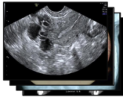
\includegraphics[height=1.5cm]{ch07/assets/example-000.png}};
\node[labeltext,anchor=west,font=\thesisfigurefont\bfseries] at (10.0,.98) {医学影像};
\node[labeltext,anchor=west,text=black!65] at (10.0,.45) {持续到达的数据};
\node[box,minimum width=2.8cm,minimum height=.6cm,fill=white] (textenc) at (3.025,-.95) {文本编码器};
\node[box,minimum width=2.8cm,minimum height=.6cm,fill=white] (imageenc) at (10.075,-.95) {图像编码器};
\draw[flow] (3.025,-.12) -- (textenc.north);
\draw[flow] (10.075,-.12) -- (imageenc.north);
\node[box,draw=modelteal,line width=1pt,fill=modelteal!5,minimum width=13.1cm,minimum height=1.55cm] (model) at (6.55,-2.48) {};
\node[labeltext,text=modelteal,font=\thesisfigurefont\bfseries] at (6.55,-2.02) {医学多模态基础模型};
\node[labeltext] at (6.55,-2.5) {影像\quad 文本\quad 结构\quad 知识};
\node[labeltext,text=black!65] at (6.55,-2.96) {跨模态融合\enspace /\enspace 共享表征\enspace /\enspace 版本记录};
\draw[flow] (textenc.south) -- (model.north -| textenc.south);
\draw[flow] (imageenc.south) -- (model.north -| imageenc.south);
\node[task] (task1) at (1.875,-5.48) {};
\node[task] (task2) at (6.55,-5.48) {};
\node[task] (task3) at (11.225,-5.48) {};
\node[labeltext,font=\thesisfigurefont\bfseries] at (1.875,-4.65) {任务一\\胸部 X 线诊断};
\node[labeltext,font=\thesisfigurefont\bfseries] at (6.55,-4.65) {任务二\\消化内镜识别};
\node[labeltext,font=\thesisfigurefont\bfseries] at (11.225,-4.65) {任务三\\皮肤镜分类};
\node[inner sep=0pt] at (1.875,-5.95) {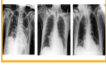
\includegraphics[height=1.35cm]{ch07/assets/example-001.png}};
\node[inner sep=0pt] at (6.55,-5.95) {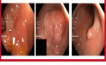
\includegraphics[height=1.35cm]{ch07/assets/example-002.png}};
\node[inner sep=0pt] at (11.225,-5.95) {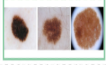
\includegraphics[height=1.35cm]{ch07/assets/example-003.png}};
\draw[flow] (model.south -| task1.north) -- (task1.north);
\draw[flow] (task1.east) -- (task2.west);
\draw[flow] (task2.east) -- (task3.west);
\node[labeltext,text=black!65] at (8.45,-3.72) {新模态、新任务、新中心与新知识};
\draw[flow,dashed,draw=modelteal!70] (3.75,-4.02) -- (13.1,-4.02);
\node[labeltext,text=black!65] at (6.55,-7.18) {顺序适配\quad $\longrightarrow$\quad 阶段评价};
\draw[draw=black!20,line width=.55pt] (0,-7.59) -- (13.1,-7.59);
\node[labeltext] at (6.55,-8.04)
  {\textbf{稳定性}\enspace 既有能力保持\qquad $\longleftrightarrow$\qquad \textbf{可塑性}\enspace 新增信息吸收};
\end{tikzpicture}
\endgroup
}
\caption[医学多模态基础模型持续学习的未来研究框架]{医学多模态基础模型持续学习的未来研究框架。持续到达的影像与文本经多模态基础模型形成共享表示，并依次适配不同影像模态、中心和下游任务。未来研究从数据与表征、任务与场景、知识与行为三个层次展开，分别对应持续预训练、参数高效持续适配和持续知识编辑。}
\label{fig:future-medical-mllm}
\end{figure}

更新对象可分别位于影像与文本表示、任务适配模块，以及模型使用的知识或规则。相应地，未来研究分为持续预训练、参数高效持续适配和持续知识编辑三个方向，并分别确定可访问历史信息、测试任务与资源需求。

\begin{figure}[htbp]
\centering
\resizebox{\textwidth}{!}{% Three research directions surround a shared objective, not a serial algorithm.
\begingroup
\linespread{1}\selectfont
\definecolor{routegreen}{HTML}{3D7166}
\definecolor{routegold}{HTML}{AB7E32}
\definecolor{routerust}{HTML}{A65D48}
\begin{tikzpicture}[
  font=\thesisfigurefont,
  direction/.style={circle,minimum size=3.75cm,draw,line width=.85pt,inner sep=0pt},
  labeltext/.style={align=center,inner sep=0pt},
  spoke/.style={-{Latex[length=2mm]},draw=black!45,line width=.75pt,shorten <=2pt,shorten >=2pt}
]
\node[direction,draw=routegreen,fill=routegreen!5] (data) at (1.95,0) {};
\node[direction,draw=routegold,fill=routegold!6] (task) at (11.15,0) {};
\node[direction,draw=routerust,fill=routerust!5] (knowledge) at (6.55,-4.2) {};
\node[labeltext,text=routegreen] at (1.95,.7) {数据与表征};
\node[labeltext,font=\thesisfigurefont\bfseries] at (1.95,.08) {持续预训练};
\node[labeltext,text=black!65] at (1.95,-.6) {新数据\quad 表征保持};
\node[labeltext,text=routegold] at (11.15,.90) {任务与场景};
\node[labeltext,font=\thesisfigurefont\bfseries] at (11.15,.02) {参数高效\\持续适配};
\node[labeltext,text=black!65] at (11.15,-.85) {新场景\quad 参数高效};
\node[labeltext,text=routerust] at (6.55,-3.5) {知识与行为};
\node[labeltext,font=\thesisfigurefont\bfseries] at (6.55,-4.12) {持续知识编辑};
\node[labeltext,text=black!65] at (6.55,-4.8) {新知识\quad 能力保持};
\node[circle,minimum size=3.05cm,draw=black!65,fill=black!3,line width=.9pt,inner sep=0pt] (goal) at (6.55,-.6) {};
\node[labeltext,font=\thesisfigurefont\bfseries] at (6.55,-.37) {医学多模态\\持续学习};
\node[labeltext,text=black!65,font=\sffamily\heiti\fontsize{10bp}{12bp}\selectfont] at (6.55,-1.12) {稳定性\,$\leftrightarrow$\,可塑性};
\draw[spoke] (goal) -- (data);
\draw[spoke] (goal) -- (task);
\draw[spoke] (goal) -- (knowledge);
\end{tikzpicture}
\endgroup
}
\caption[医学多模态基础模型持续学习的三层研究路线]{医学多模态基础模型持续学习的三层研究路线。持续预训练更新影像与文本表示，参数高效持续适配处理中心和任务变化，持续知识编辑修订经审核的知识与输出规则。MedCL 的后续实现拟记录模型版本，并比较各版本的历史能力与新增能力。}
\label{fig:future-three-level-roadmap}
\end{figure}

\subsection{数据与表征层：持续预训练与表征保持}

持续预训练需要在吸收新影像和新报告时，保留已有器官结构、疾病相关视觉特征和影像--文本对应关系。可在历史访问受限条件下，比较少量历史样本、旧模型输出和压缩表征对这些能力的保持效果。

这一层次需要建立带有时间与来源记录的数据流，区分采集时间、报告版本、患者划分和来源中心。对于影像与报告不完全配对或部分模态缺失的情况，应分别评价单模态能力和跨模态匹配，避免以样本数量增长替代数据质量分析。少量代表性历史样本、旧模型输出或压缩表征可作为知识保持的候选载体，但其存储成本、信息保真和共享限制需要在相同条件下比较。

评价包括固定历史任务、新任务迁移和跨模态匹配。分割、分类和配准用于检查结构与语义表示，影像检索和图文对应用于检查跨模态关联。各更新版本与未更新模型及相同新增数据下的直接训练模型比较，并报告训练步数、显存与历史信息存储量。

\subsection{任务与场景层：参数高效持续适配}

新中心的设备、患者构成、标注规范和下游用途可能与既有数据不同。后续可研究低秩适配、提示或小型任务模块，在限制可训练参数数量的条件下持续适应新场景，并结合历史特征保持、子空间保护或有限回放。

当数据未标明任务切换时点，且旧中心可能再次出现时，需要判断何时更新、何时复用已有适配模块，以及何时增加新模块。评价同时记录任务或模块选择错误及模块数量增长。联邦环境还需区分本地适应与跨客户端共享，研究哪些更新适合在客户端之间交换。

在固定基础模型、数据划分和训练预算的条件下，比较完整微调、独立适配与持续适配，并分别记录可训练参数数量、计算量和存储开销。除新中心性能外，评价旧中心保持、未知中心泛化和模块选择错误；联邦设置还报告通信量与客户端参与情况。

\subsection{知识与行为层：持续知识编辑与能力保持}

经审核的医学知识、术语或输出规则发生变化时，可研究针对性的连续编辑，更新指定内容并保持无关知识及已有任务能力。重点比较连续多次编辑的累积影响，以及影像概念与文字描述之间的对应关系是否发生非预期变化。

对于医学多模态模型，编辑目标既可能涉及文本知识，也可能涉及影像概念与文字描述之间的对应关系。需要区分更新外部检索资料、修改提示或规则以及直接修改模型参数三种方式，分别说明修改作用于哪一层、何时生效以及能否撤回。新增知识条目应具有可核验来源和版本；涉及医学判断的更新还需要相应专业审核，不能仅以模型生成的新回答作为修改正确性的依据。

评价可围绕编辑目标的正确性、同义提问和相关影像上的泛化、无关知识与旧任务保持，以及连续编辑后的累积干扰展开。对于证据不足的输入，还应检查模型是否保留适当的不确定性表达和人工复核入口。本文尚未开展知识编辑实验，后续需先建立明确的编辑集合、未编辑对照和历史能力测试，再判断局部更新是否带来可接受的能力变化。

\subsection{MedCL 的实现与验证}

MedCL 后续可接收外部更新后的模型或预测，在固定测试集上比较不同版本。持续预训练、持续适配和知识编辑分别报告表示保持、新旧场景表现，以及指定修改的正确性和影响范围。

平台实现优先完成基准选择、阶段配置、模型或预测提交、独立评分和报告生成。验证内容包括样本匹配、任务身份与分类头选择、配准坐标约定、缺失阶段处理，以及模型推理和上传文件的安全检查。联邦评价按固定客户端测试分组评分。各项后续算法研究独立训练，其模型或预测按规定格式提交评测。


\backmatter
\begingroup
\setlength{\emergencystretch}{2em}
\setlength{\bibsep}{0.5\baselineskip}
\interlinepenalty=10000
\raggedbottom
\bibliographystyle{bibliography/thesis-plainnat}
\bibliography{bibliography/references}
\endgroup
\chapter*{攻读博士期间学术成果}
\label{back:publications}
\setlength{\emergencystretch}{2em}

\section*{第一作者或共同第一作者(*)论文}

\subsection*{已发表论文}
\begin{enumerate}[leftmargin=2.3em,label={[\arabic*]},itemsep=0.55em,topsep=0.4em]
  \item \textbf{Wang B}$^{*}$, Luo X$^{*}$, Zhuang X. Toward universal medical image registration via sharpness-aware meta-continual learning. In \emph{Medical Image Computing and Computer Assisted Intervention}, pages 739--748, 2024.

  \item Zhang K$^{*}$, \textbf{Wang B}$^{*}$, Zhou H, Zhuang X. ZScribbleSeg: A comprehensive segmentation framework with modeling of efficient annotation and maximization of scribble supervision. \emph{Medical Image Analysis}, 112:104074, 2026.
\end{enumerate}

\subsection*{审稿中论文}
\begin{enumerate}[leftmargin=2.3em,label={[\arabic*]},itemsep=0.55em,topsep=0.4em,resume]
  \item \textbf{Wang B}$^{*}$, Zhou H$^{*}$, Gao Y, Zhuang X. Beyond forgetting in continual medical image segmentation: A comprehensive benchmark study. 投稿至\emph{IEEE Transactions on Pattern Analysis and Machine Intelligence}.

  \item \textbf{Wang B}, Zhou H, Gao Y, Gao S, Zhuang X. FedSubMerge: Subspace merging for replay-free federated continual medical image classification. 投稿至\emph{IEEE Transactions on Medical Imaging}.

  \item Jiang S$^{*}$, \textbf{Wang B}$^{*}$, Zhou H$^{*}$, Feng J, Zhuang X. Engram neuron inspired adaptive memorization for lifelong learning. 投稿至\emph{CAAI Transactions on Intelligence Technology}.
\end{enumerate}

\section*{发明专利}

\begin{enumerate}[
  leftmargin=2.3em,
  label={[\arabic*]},
  itemsep=0.55em,
  topsep=0.4em
]
  \item 庄吓海, \textbf{王波民}, 周杭琪.
  一种基于子空间聚合的联邦增量学习方法、电子设备及程序产品:
  202610911538.0[P].
\end{enumerate}


\section*{其他参与论文}


\begin{enumerate}[leftmargin=2.3em,label={[\arabic*]},itemsep=0.55em,topsep=0.4em]
  \item Wan K, \textbf{Wang B}, Wu F, Gong H, Zhuang X. Context-guided continual reinforcement learning for landmark detection with incomplete data. In \emph{Medical Image Computing and Computer Assisted Intervention}, pages 157--166, 2024.

  \item Gao Y, Gao Z, Gao X, Liu Y, \textbf{Wang B}, Zhuang X. Evidential concept embedding models: Towards reliable concept explanations for skin disease diagnosis. In \emph{Medical Image Computing and Computer Assisted Intervention}, pages 308--317, 2024.

  \item Gao Y, Zhou H, Gao Z, \textbf{Wang B}, Gao S, Wang S, Zhuang X. Learning concept-driven logical rules for interpretable and generalizable medical image classification. In \emph{Medical Image Computing and Computer Assisted Intervention}, pages 291--300, 2025.

  \item Gao S, Wang S, Gao Y, \textbf{Wang B}, Zhuang X, et al. Evaluating foundation models with pathological concept learning for kidney cancer. In \emph{MICCAI Applications of Medical Artificial Intelligence}, pages 32--41, 2025.

  \item Zhou H, \textbf{Wang B}, Zhuang X. ConceptIL: Concept incremental learning for interpretable medical AI. In \emph{Medical Image Computing and Computer Assisted Intervention}, 2026（已录用）.

\end{enumerate}

\include{chapters/acknowledgements}
\cleardoublepage
\cleardoublepage
\pagestyle{empty}
	\newgeometry{
			hcentering,
			nomarginpar,
			centering,
			top=30mm,
			bottom=25mm,
			left=26mm,
			right=26mm,
			headheight=5mm,
			headsep=5mm,
			footskip=7.5mm}
\vspace{3.5cm}

\centerline{\zihao{-2} \heiti{复旦大学}}

\vspace{0.5cm}

\centerline{\zihao{-2} \heiti{学位论文独创性声明}}

\vspace{1cm}

本人郑重声明：所呈交的学位论文，是本人在导师的指导下，独立进行研究工作所取得的成果。
论文中除特别标注的内容外，不包含任何其他个人或机构已经发表或撰写过的研究成果。
对本研究做出重要贡献的个人和集体，均已在论文中作了明确的声明并表示了谢意。
本声明的法律结果由本人承担。

\vspace{2cm}

\hfill 作者签名:\underline{\hbox to 25mm{}}
\quad 日期: \underline{\hbox to 25mm{}}\hbox to 2em{}

\vspace{3cm}

\centerline{\zihao{-2} \heiti{复旦大学}}

\vspace{0.5cm}

\centerline{\zihao{-2} \heiti{学位论文使用授权声明}}

\vspace{1cm}

本人完全了解复旦大学有关收藏和利用博士、硕士学位论文的规定，
即：学校有权收藏、使用并向国家有关部门或机构送交论文的印刷本和电子版本；
允许论文被查阅和借阅；学校可以公布论文的全部或部分内容，
可以采用影印、缩印或其它复制手段保存论文。
涉密学位论文在解密后遵守此规定。


\vspace{2cm}

\hfill 作者签名:\underline{\hbox to 25mm{}}
\quad 导师签名:\underline{\hbox to 25mm{}}
\quad 日期: \underline{\hbox to 25mm{}}\hbox to 2em{}


\end{document}
